
\section{Pyörävaellus 9.–12.5.}

\begin{Figure}
	\noindent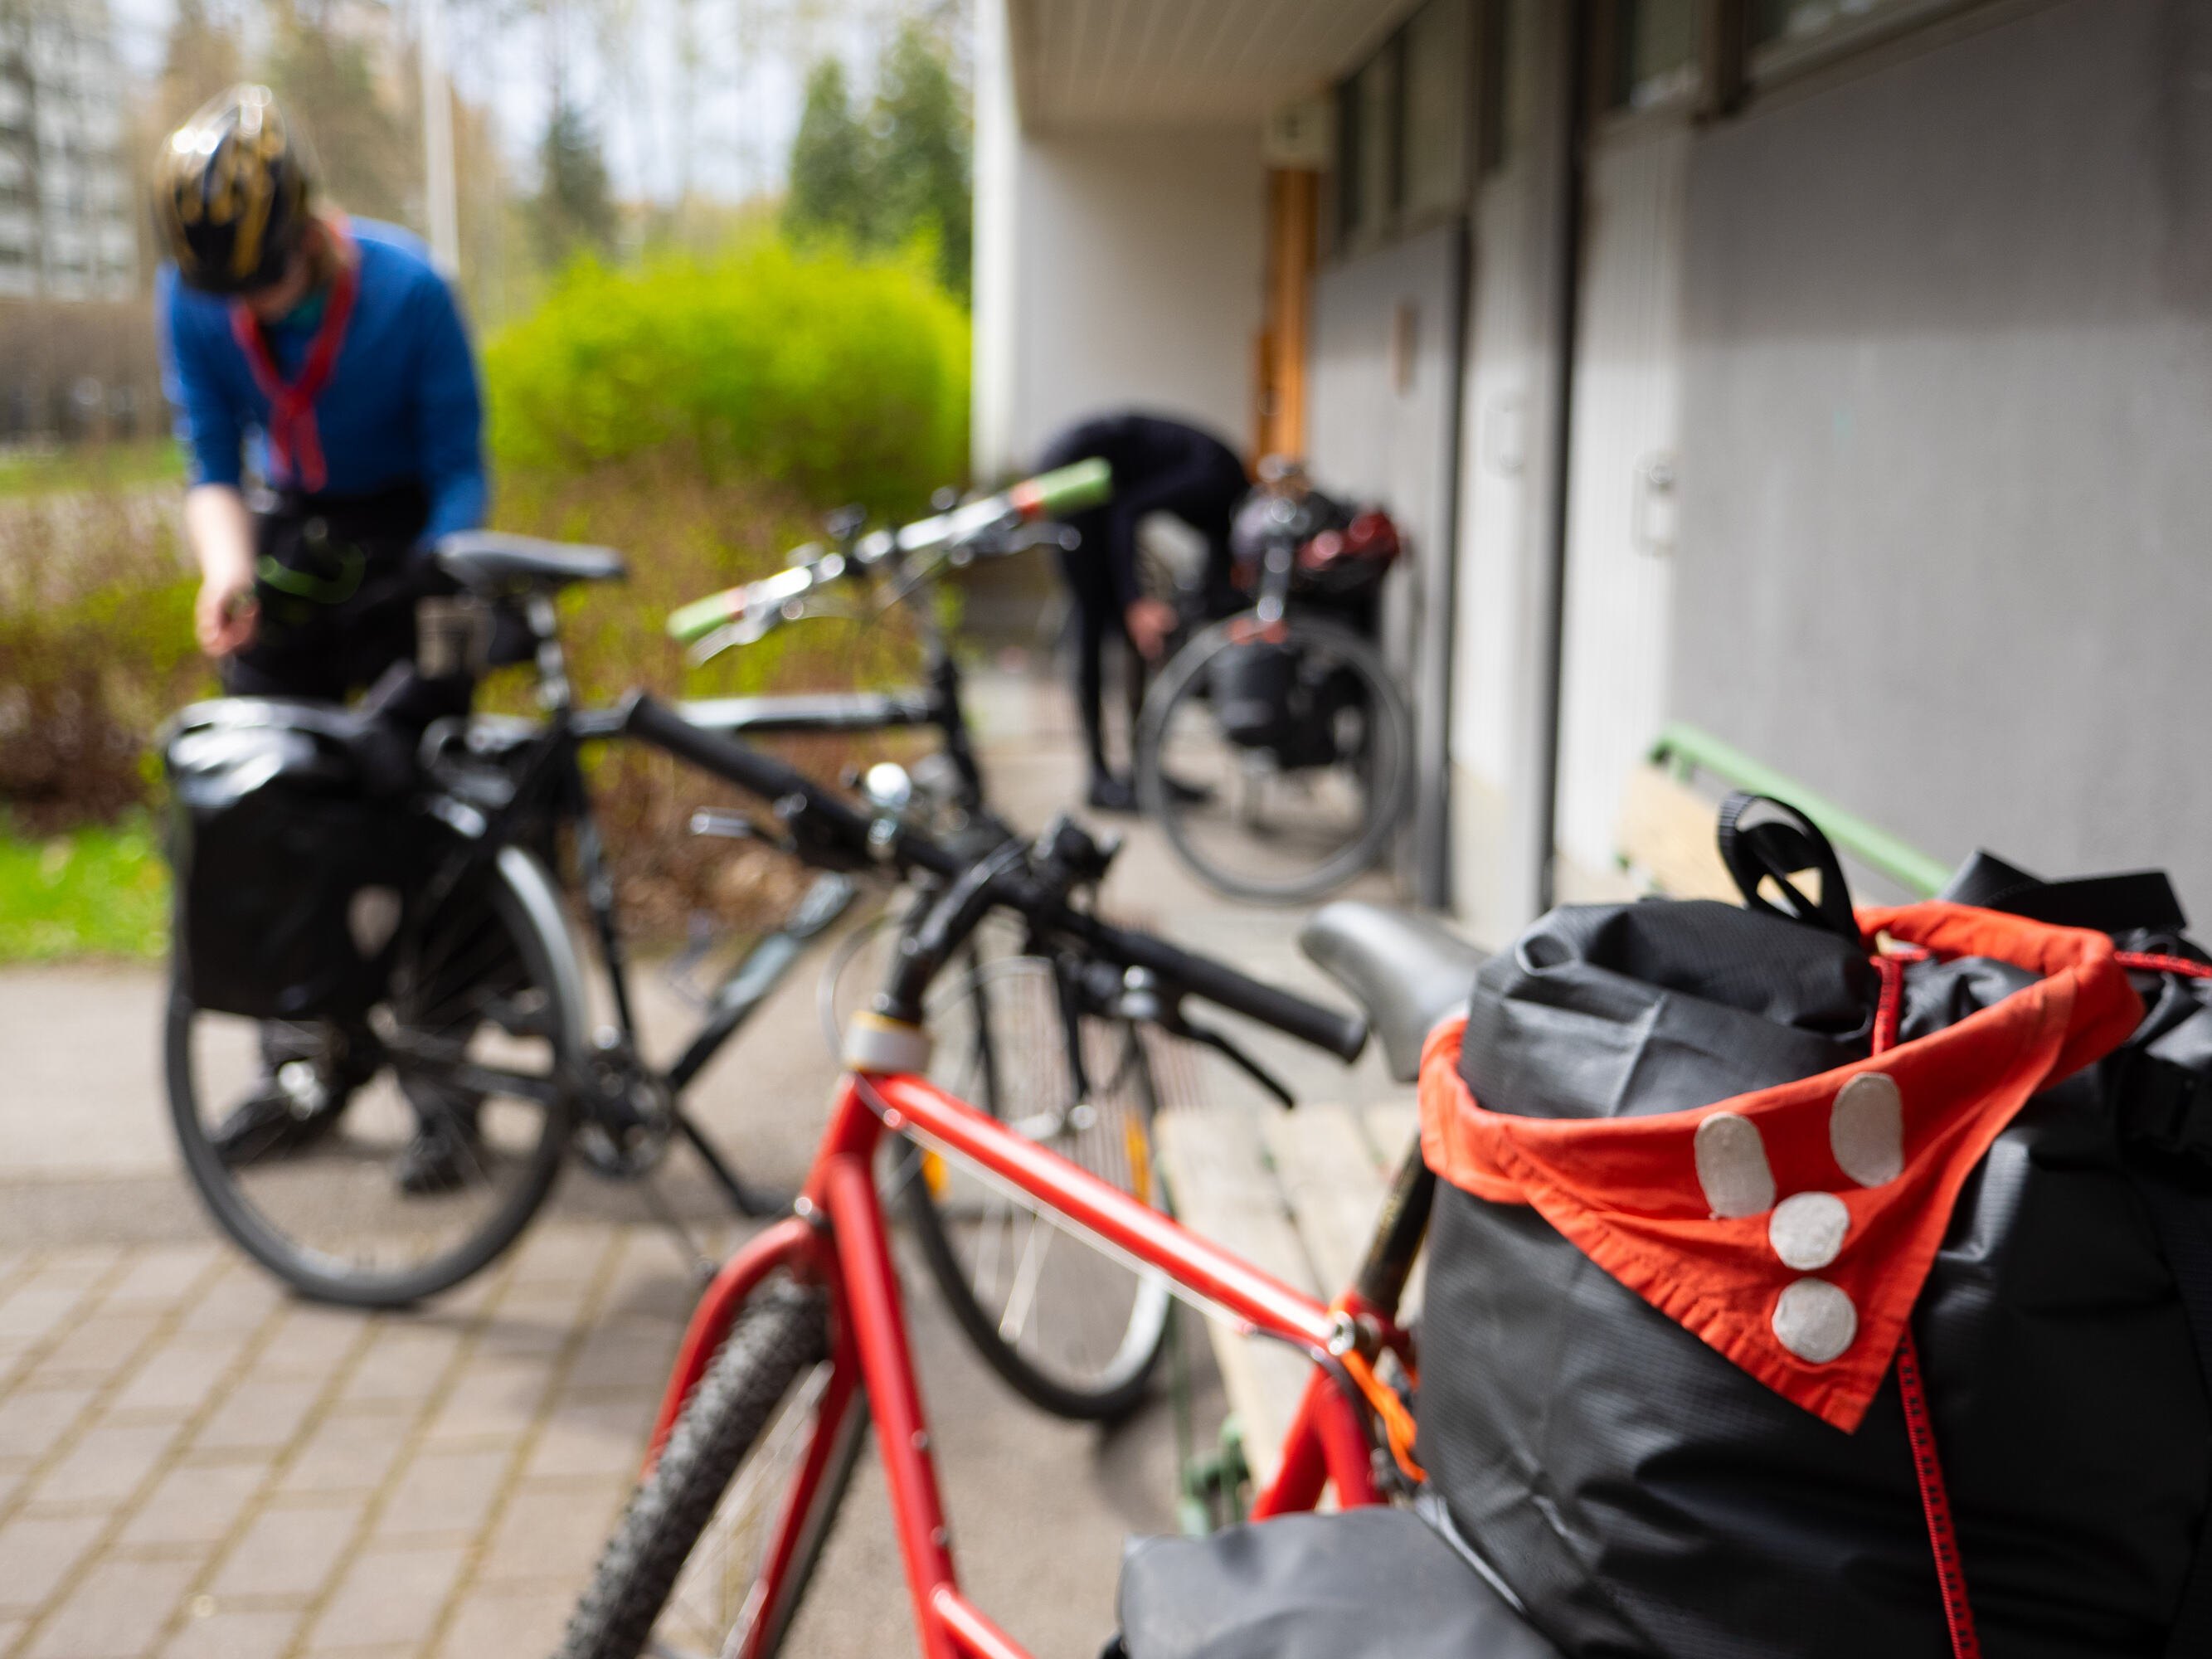
\includegraphics[width=\linewidth]{assets/pyörävaellus1}
	\captionof{figure}{Kolme rusakkoa lähtivät pyöräilemään KuRu:n
	varastolta torstaina 9.5. aamuna, läntä kohti. Ensimmäinen tekninen
	vika ilmestyi jo 600 metrin jälkeen, ja nopeasti korjaantui.}
\end{Figure}

\begin{multicols}{2}
	\begin{Figure}
		\noindent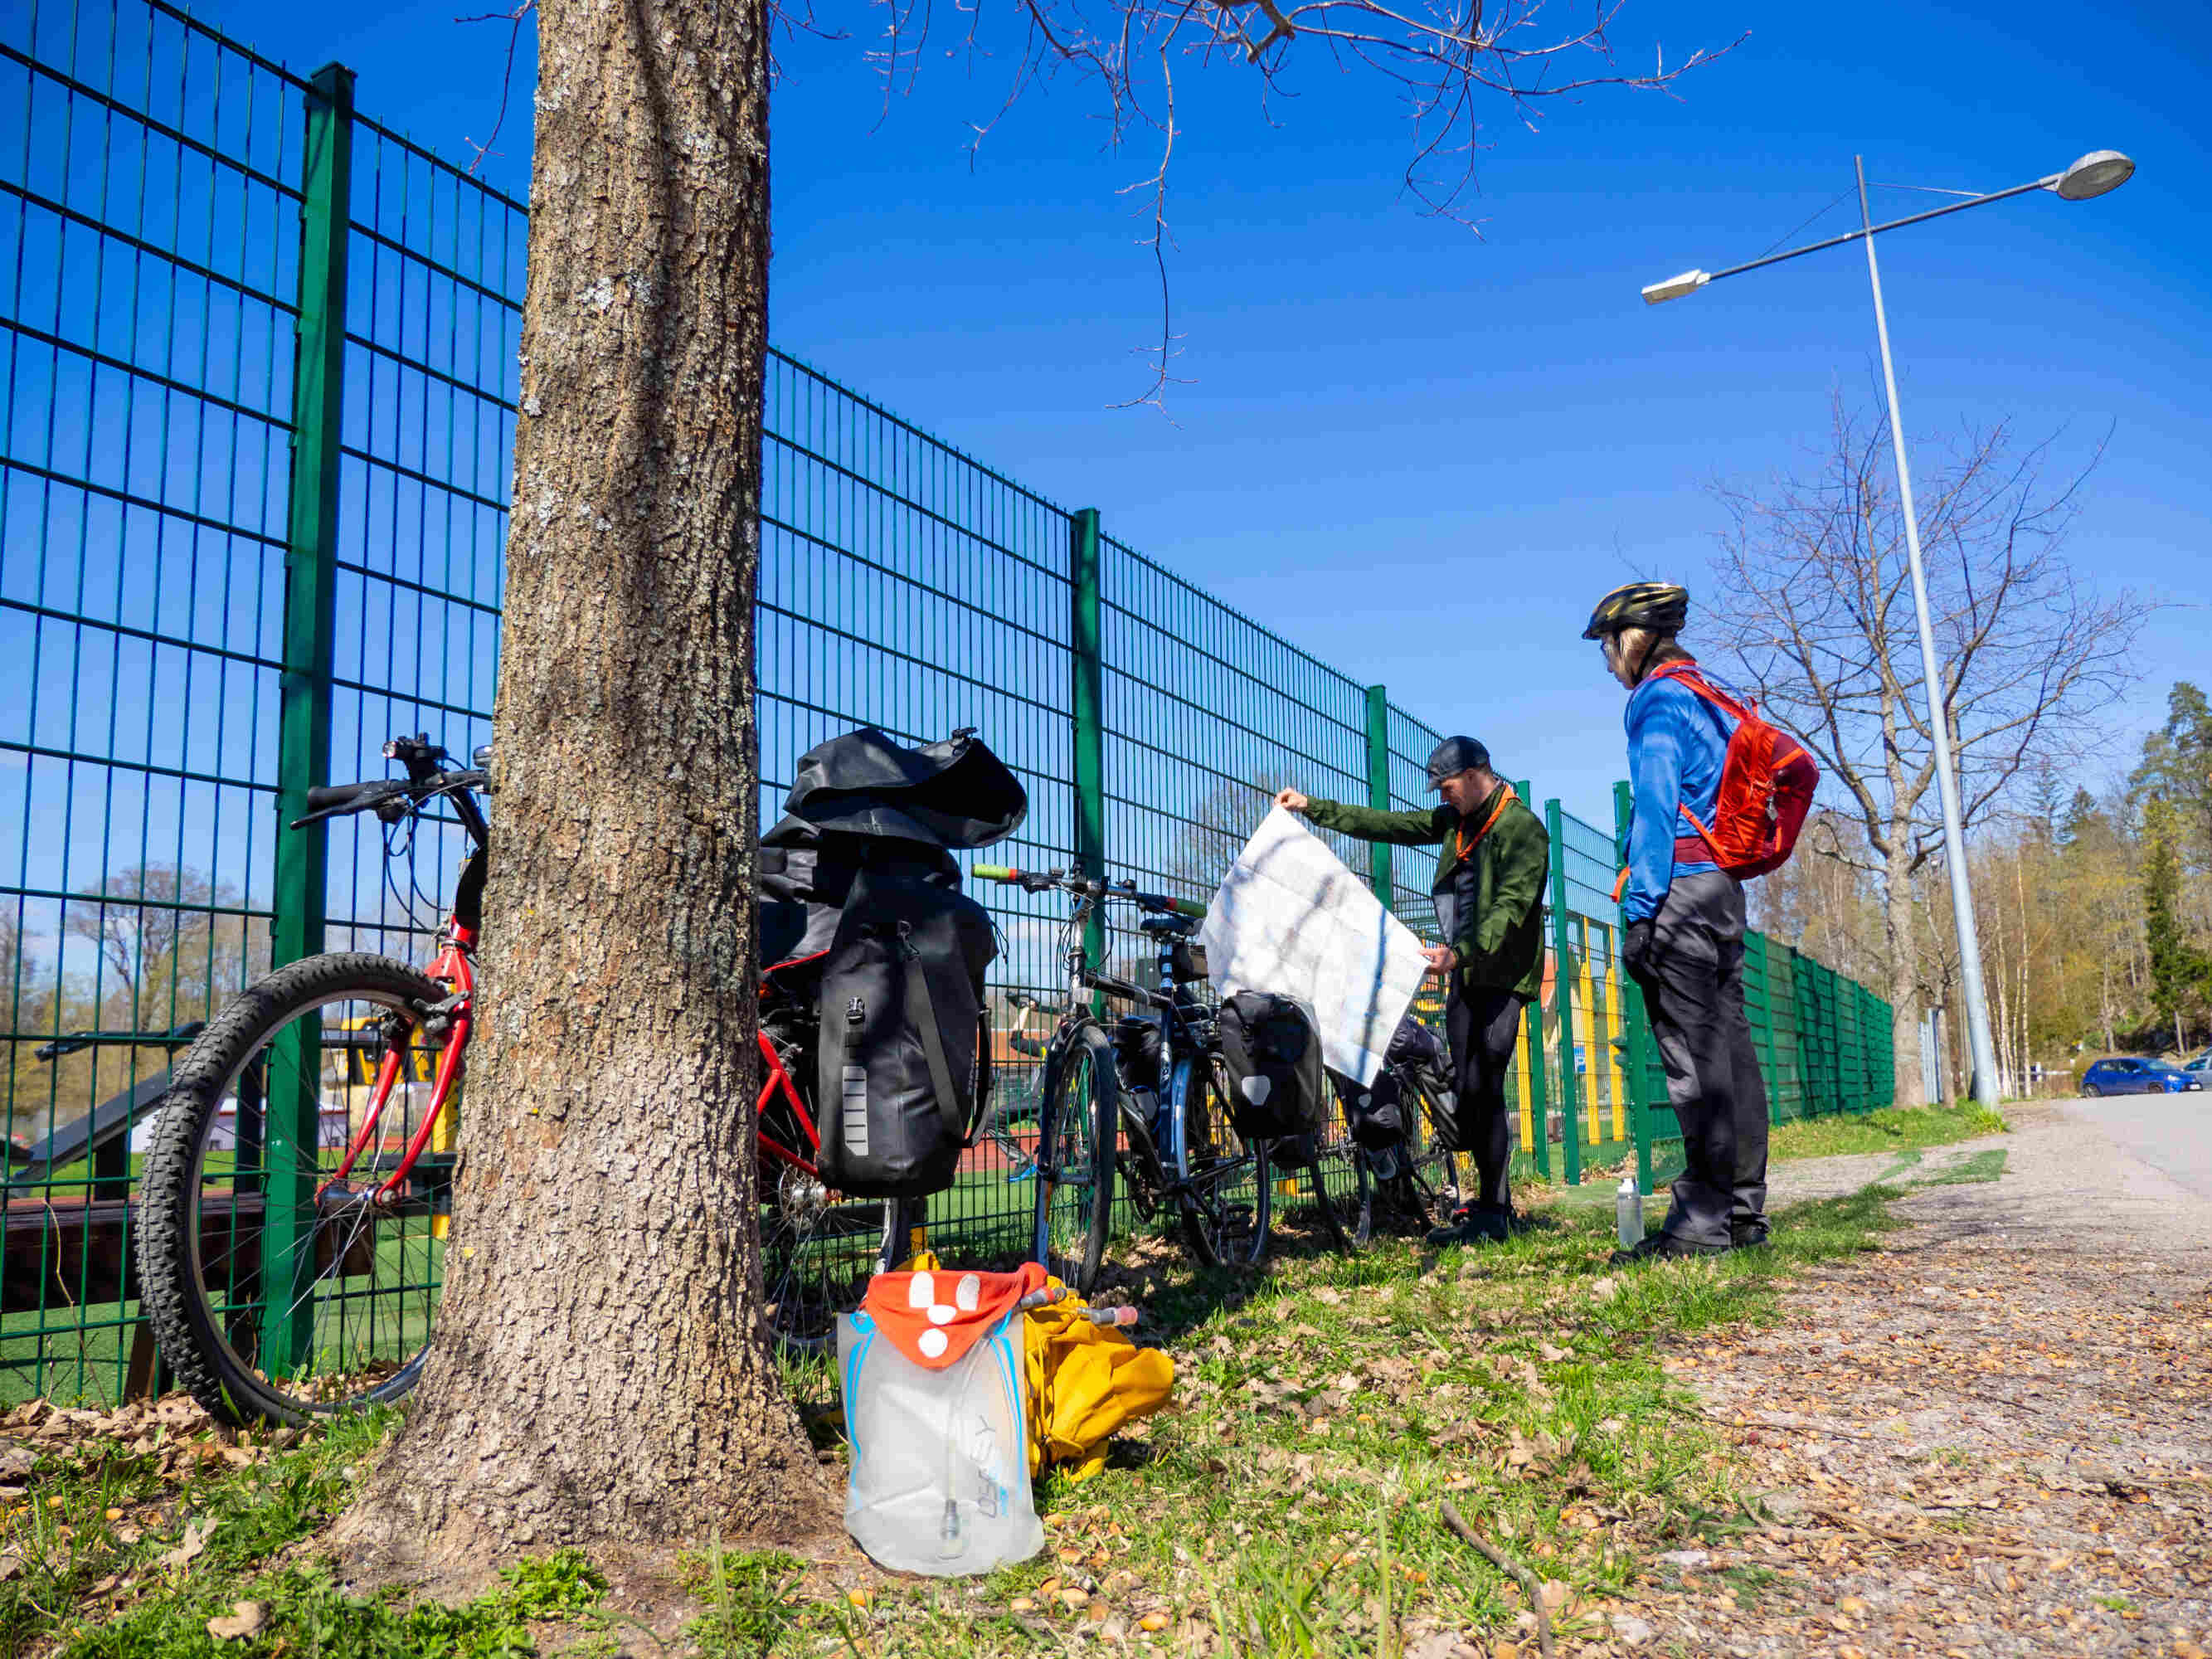
\includegraphics[width=\linewidth]{assets/pyörävaellus3}
		\captionof{figure}{Ensimmäiseksi lounaspaikaksi valittiin
		Klauklahden urheilukenttä, jonka jälkeen matka jatkui Kirkkonummen kautta.}
	\end{Figure}
	\columnbreak
	\begin{Figure}
		\noindent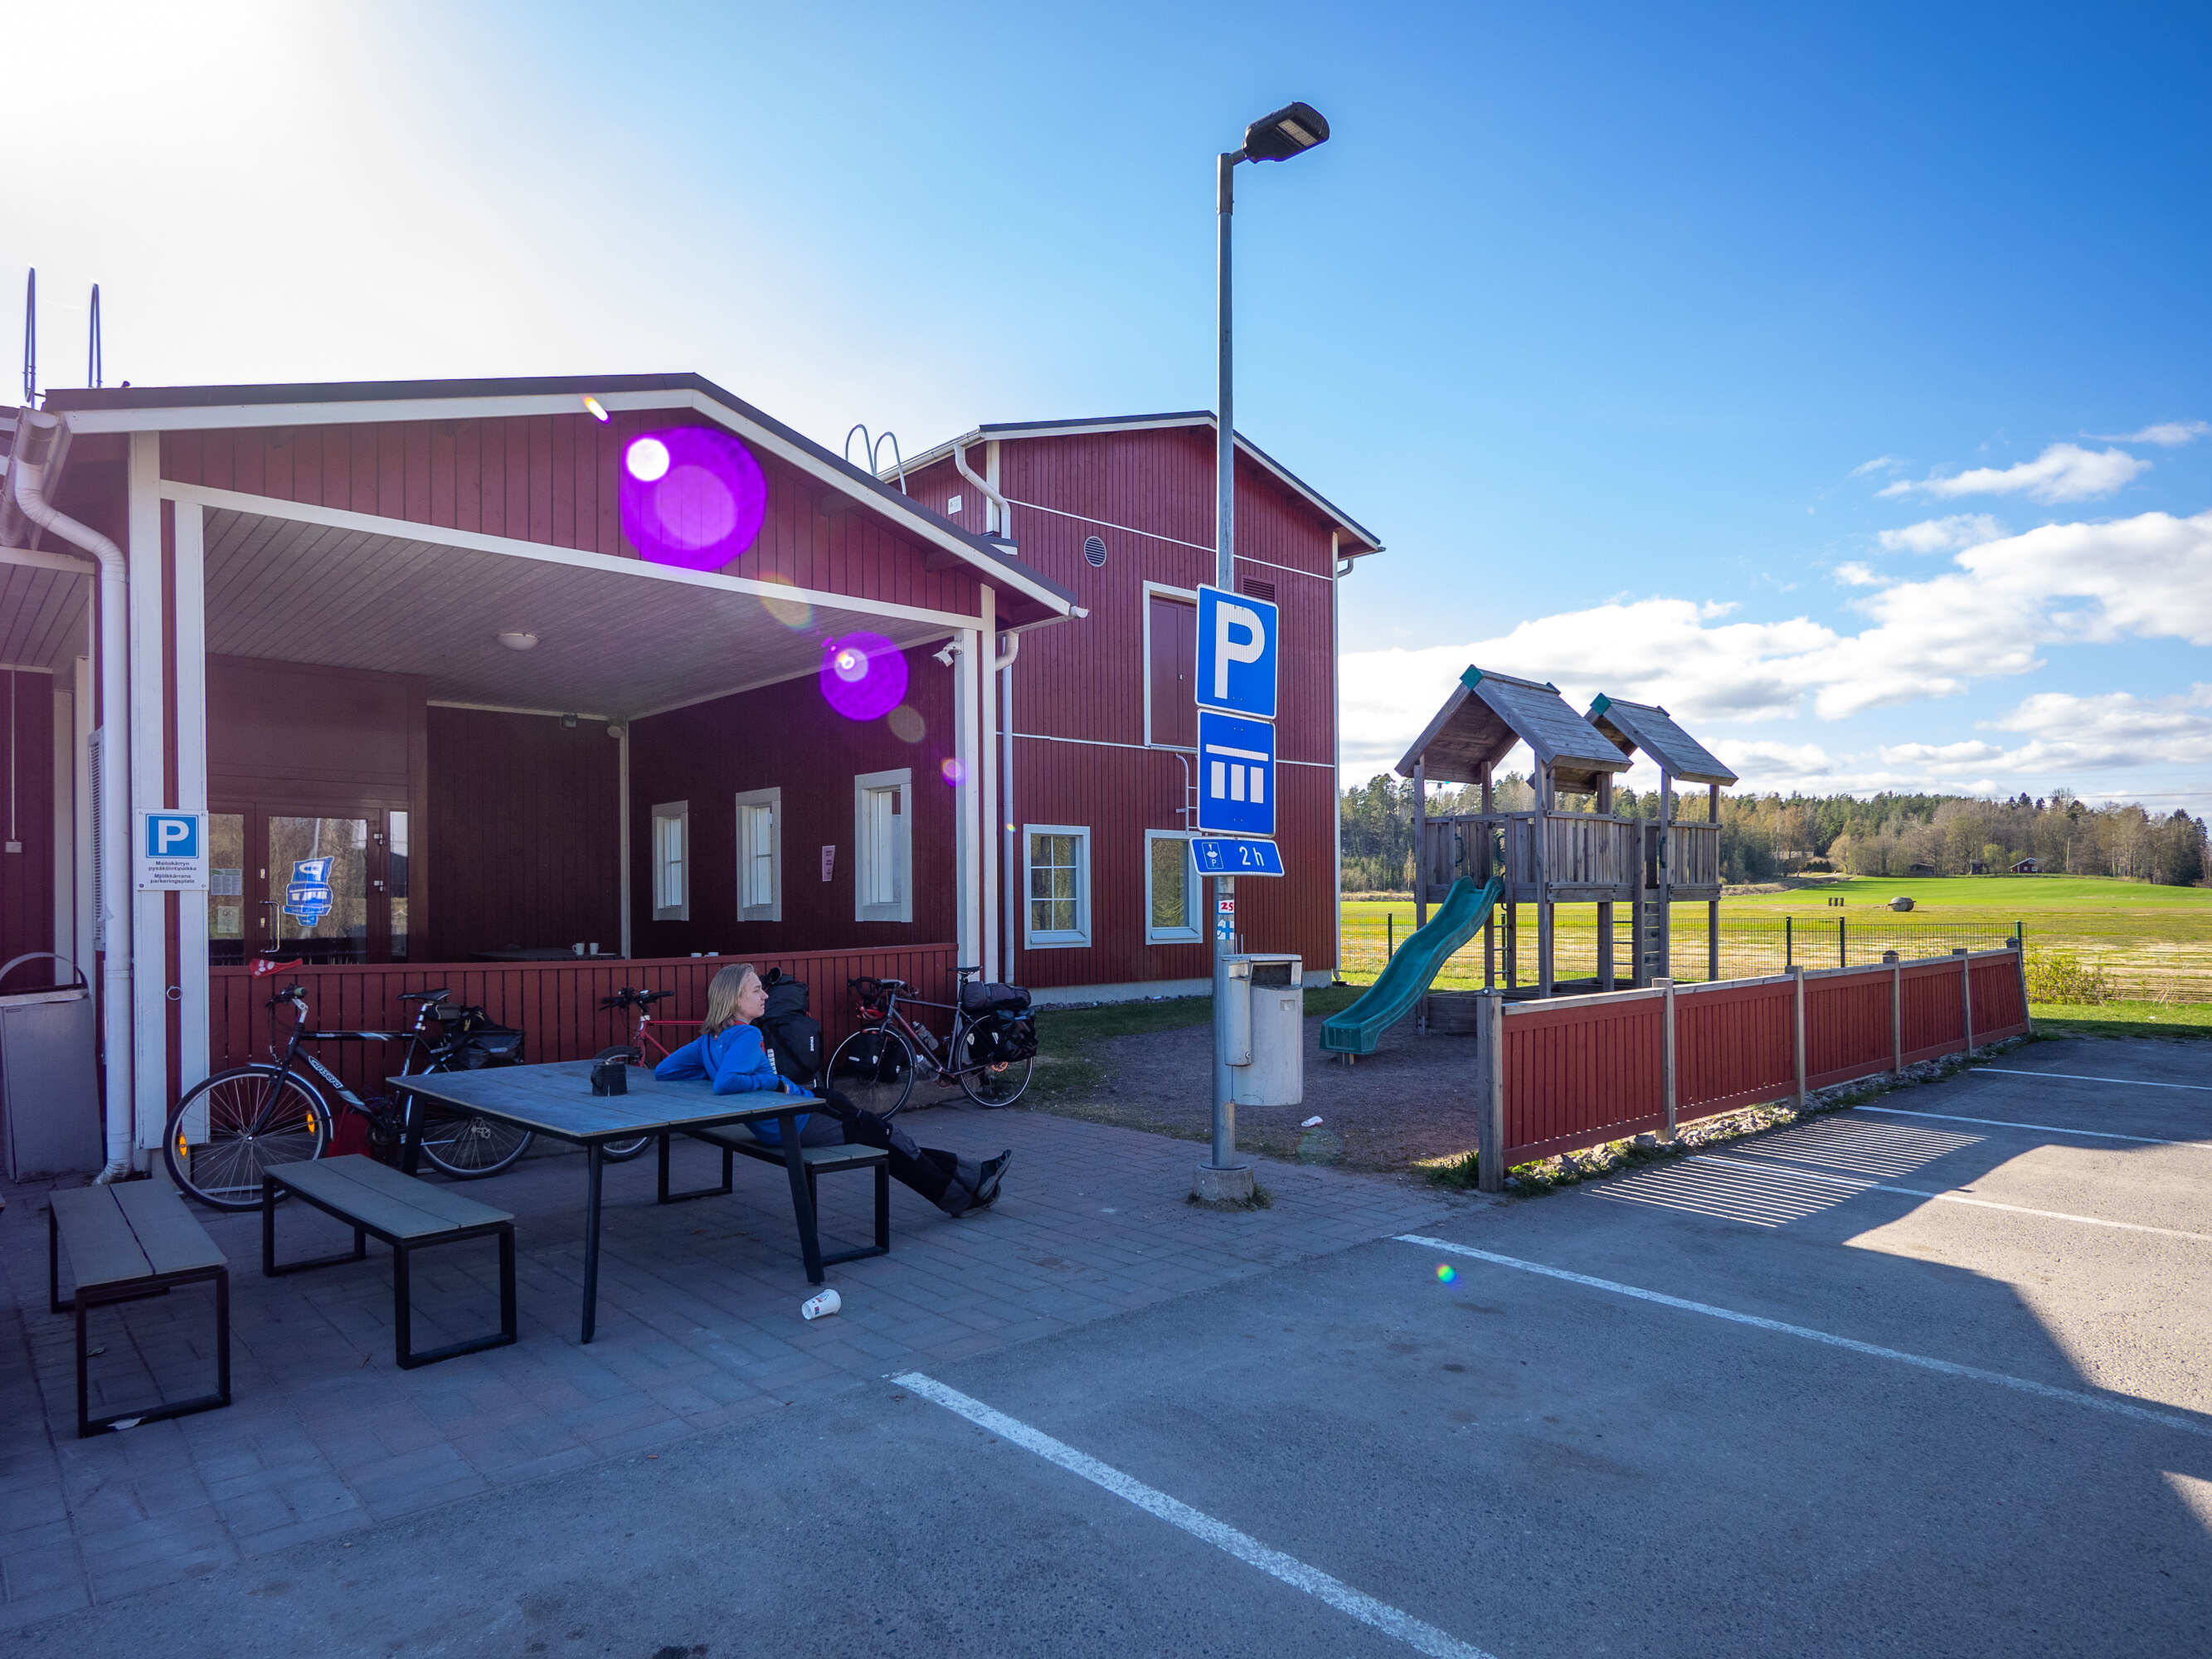
\includegraphics[width=\linewidth]{assets/pyörävaellus4}
		\captionof{figure}{Vaelluksen ensimmäinen jäätelö syötiin
		sitten Pickalan huoltoasemalla, noin 10km meidän
		päämäärästämme.}
	\end{Figure}
\end{multicols}

\begin{Figure}
	\noindent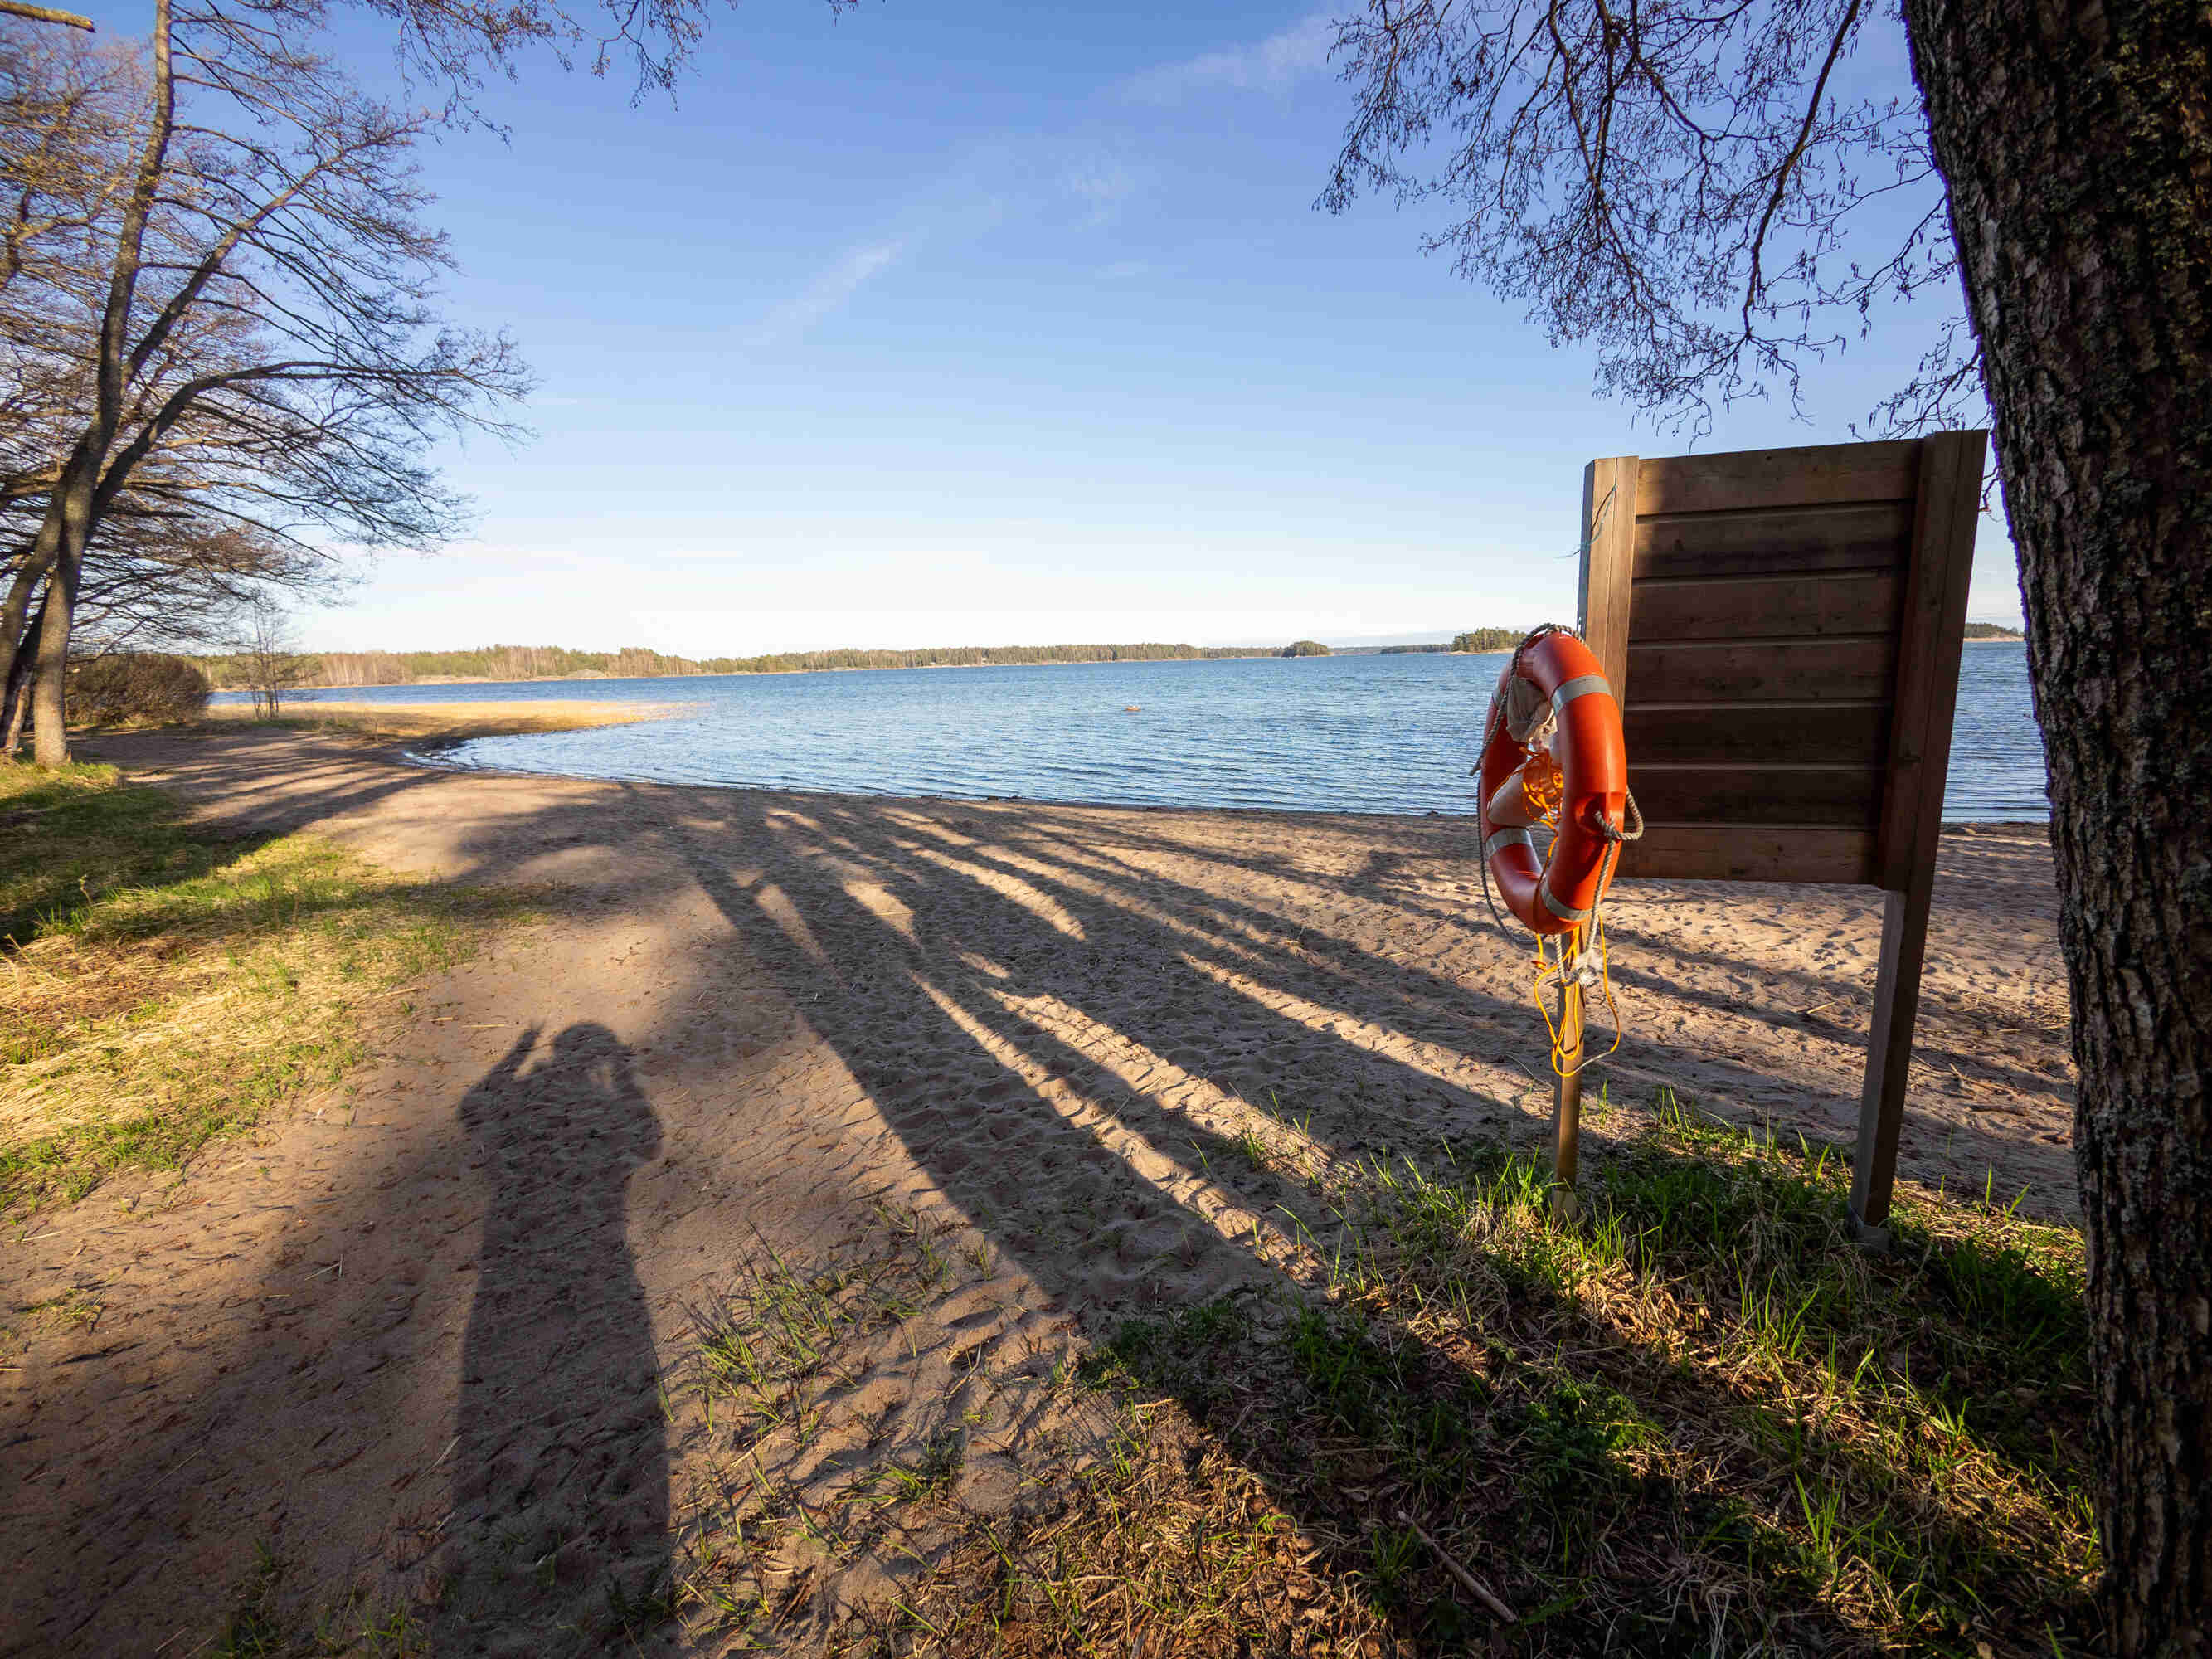
\includegraphics[width=\linewidth]{assets/pyörävaellus5}
	\captionof{figure}{Pieni mutta stressaava Inkoon Rannikkotien
	pätkä odotti meitä, jota seurasi rennompi mutta kuoppainen
	hiekkatie, ja vihdoin löytyi meidän yöpymispaikka: Kopparnäs,
	Inkoo}
\end{Figure}

\begin{multicols}{2}
	\begin{Figure}
		\noindent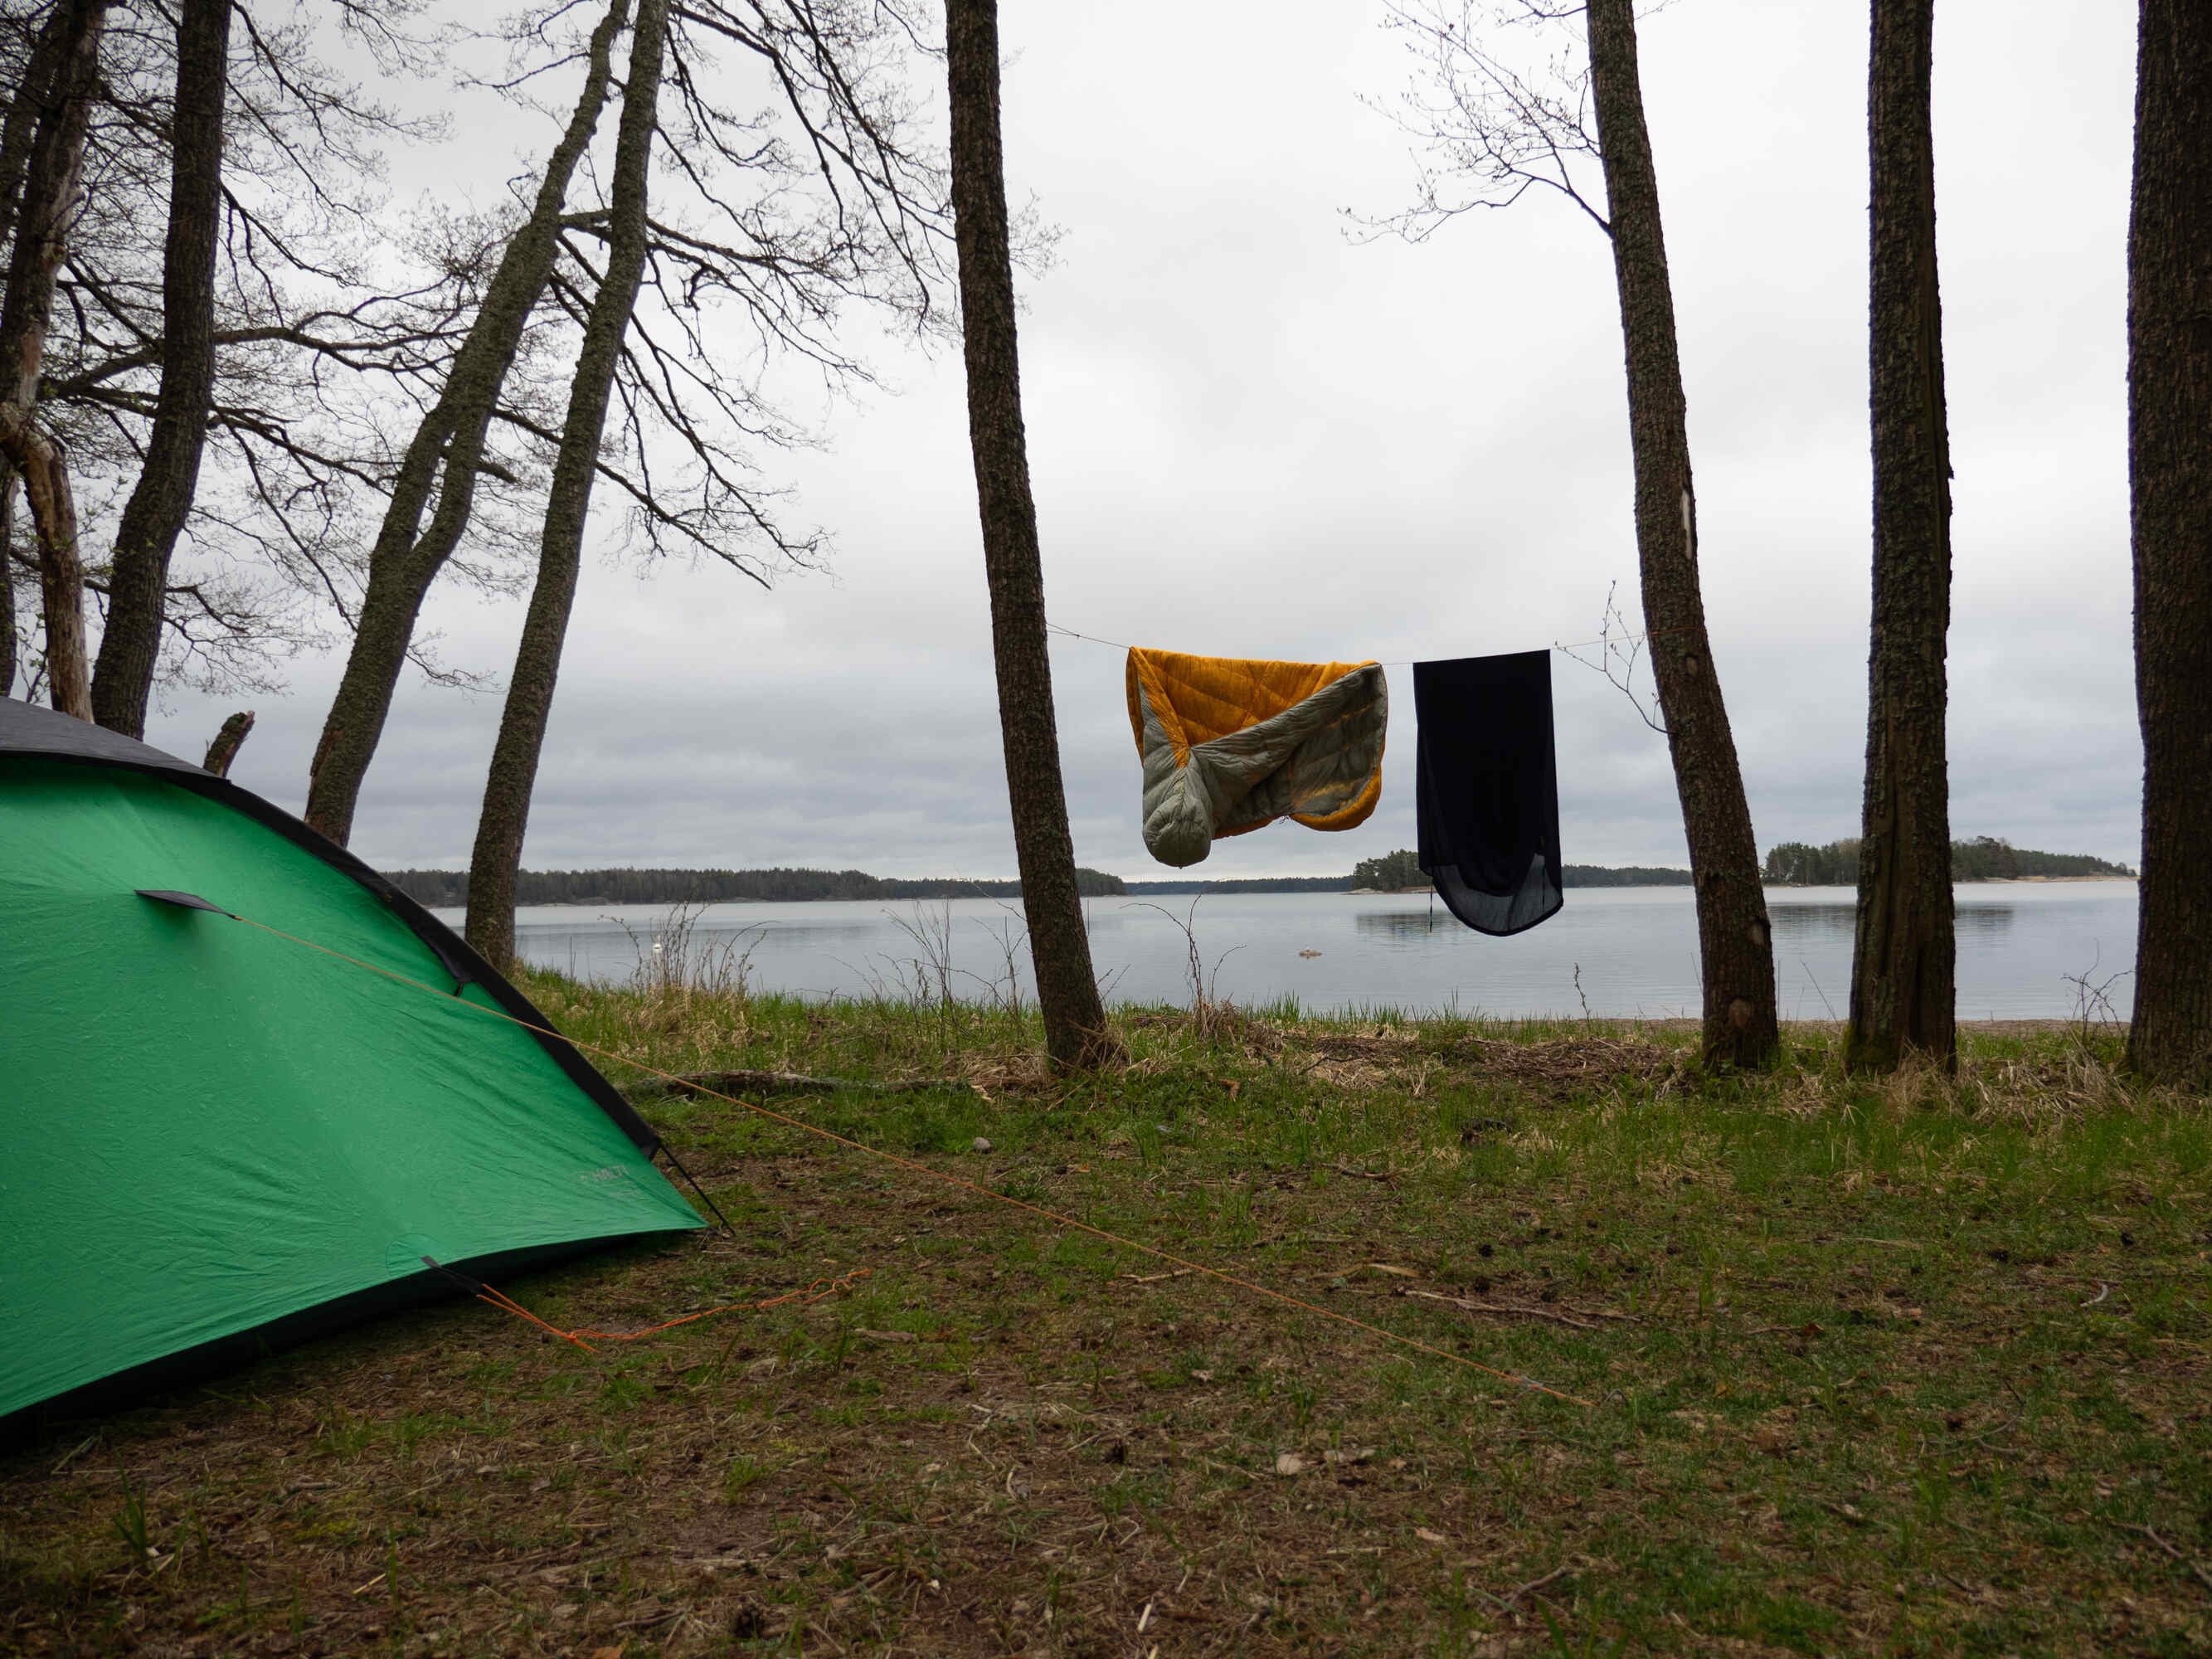
\includegraphics[width=\linewidth]{assets/pyörävaellus6}
		\captionof{figure}{74km jälkeen jotkut rusakoista alkoivat
		tuntea \textbf{vähän} kipua ja \textbf{vähän} väsymystä.
		Äänekkäät kalatiirat rannalla uhkasivat olla antamatta meidän
		nukkua, mutta onneksi lähtivät illallisen jälkeen. Sade saapui
		yöllä, ja kiltisti lähti ennen herätys.}
	\end{Figure}
	\columnbreak
	\begin{Figure}
		\noindent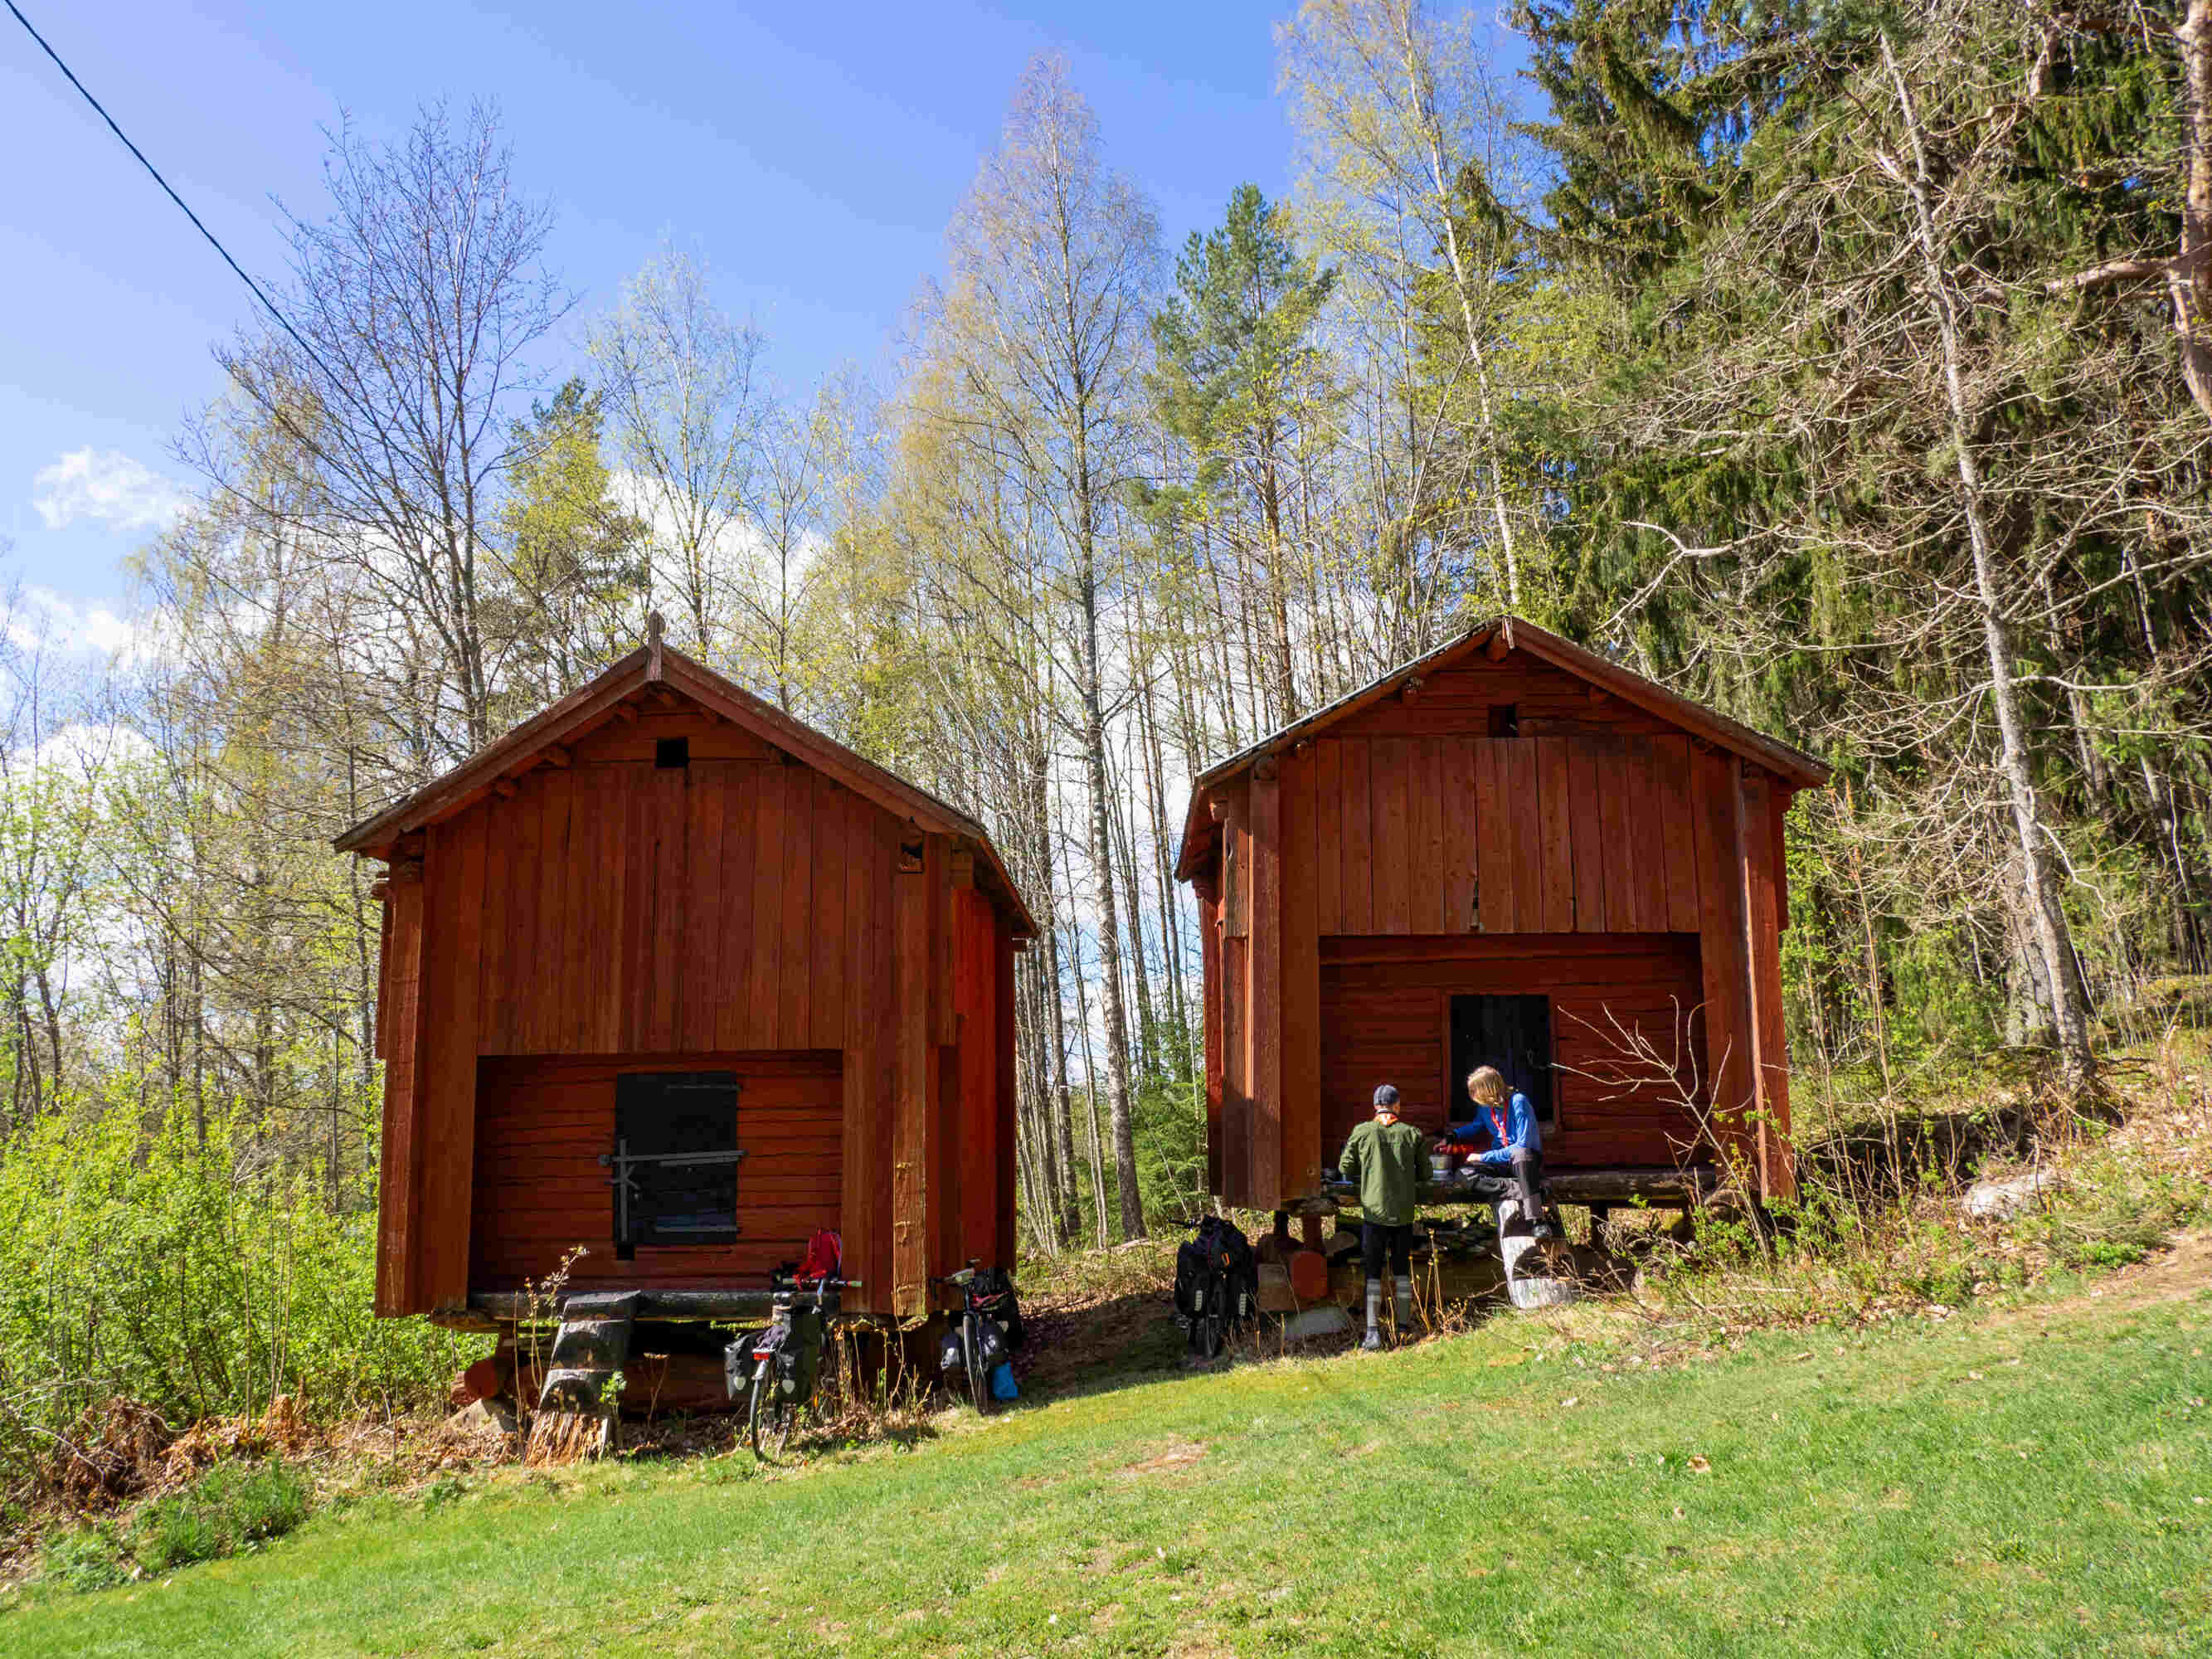
\includegraphics[width=\linewidth]{assets/pyörävaellus7}
		\captionof{figure}{Toinen päivä toi meidät pohjoiseen, päämääräna Lohja.
		Lounas syötiin noin puolivälissä, Siuntion kotiseutumuseossa.}
	\end{Figure}
\end{multicols}


\begin{Figure}
\begin{center}
	\noindent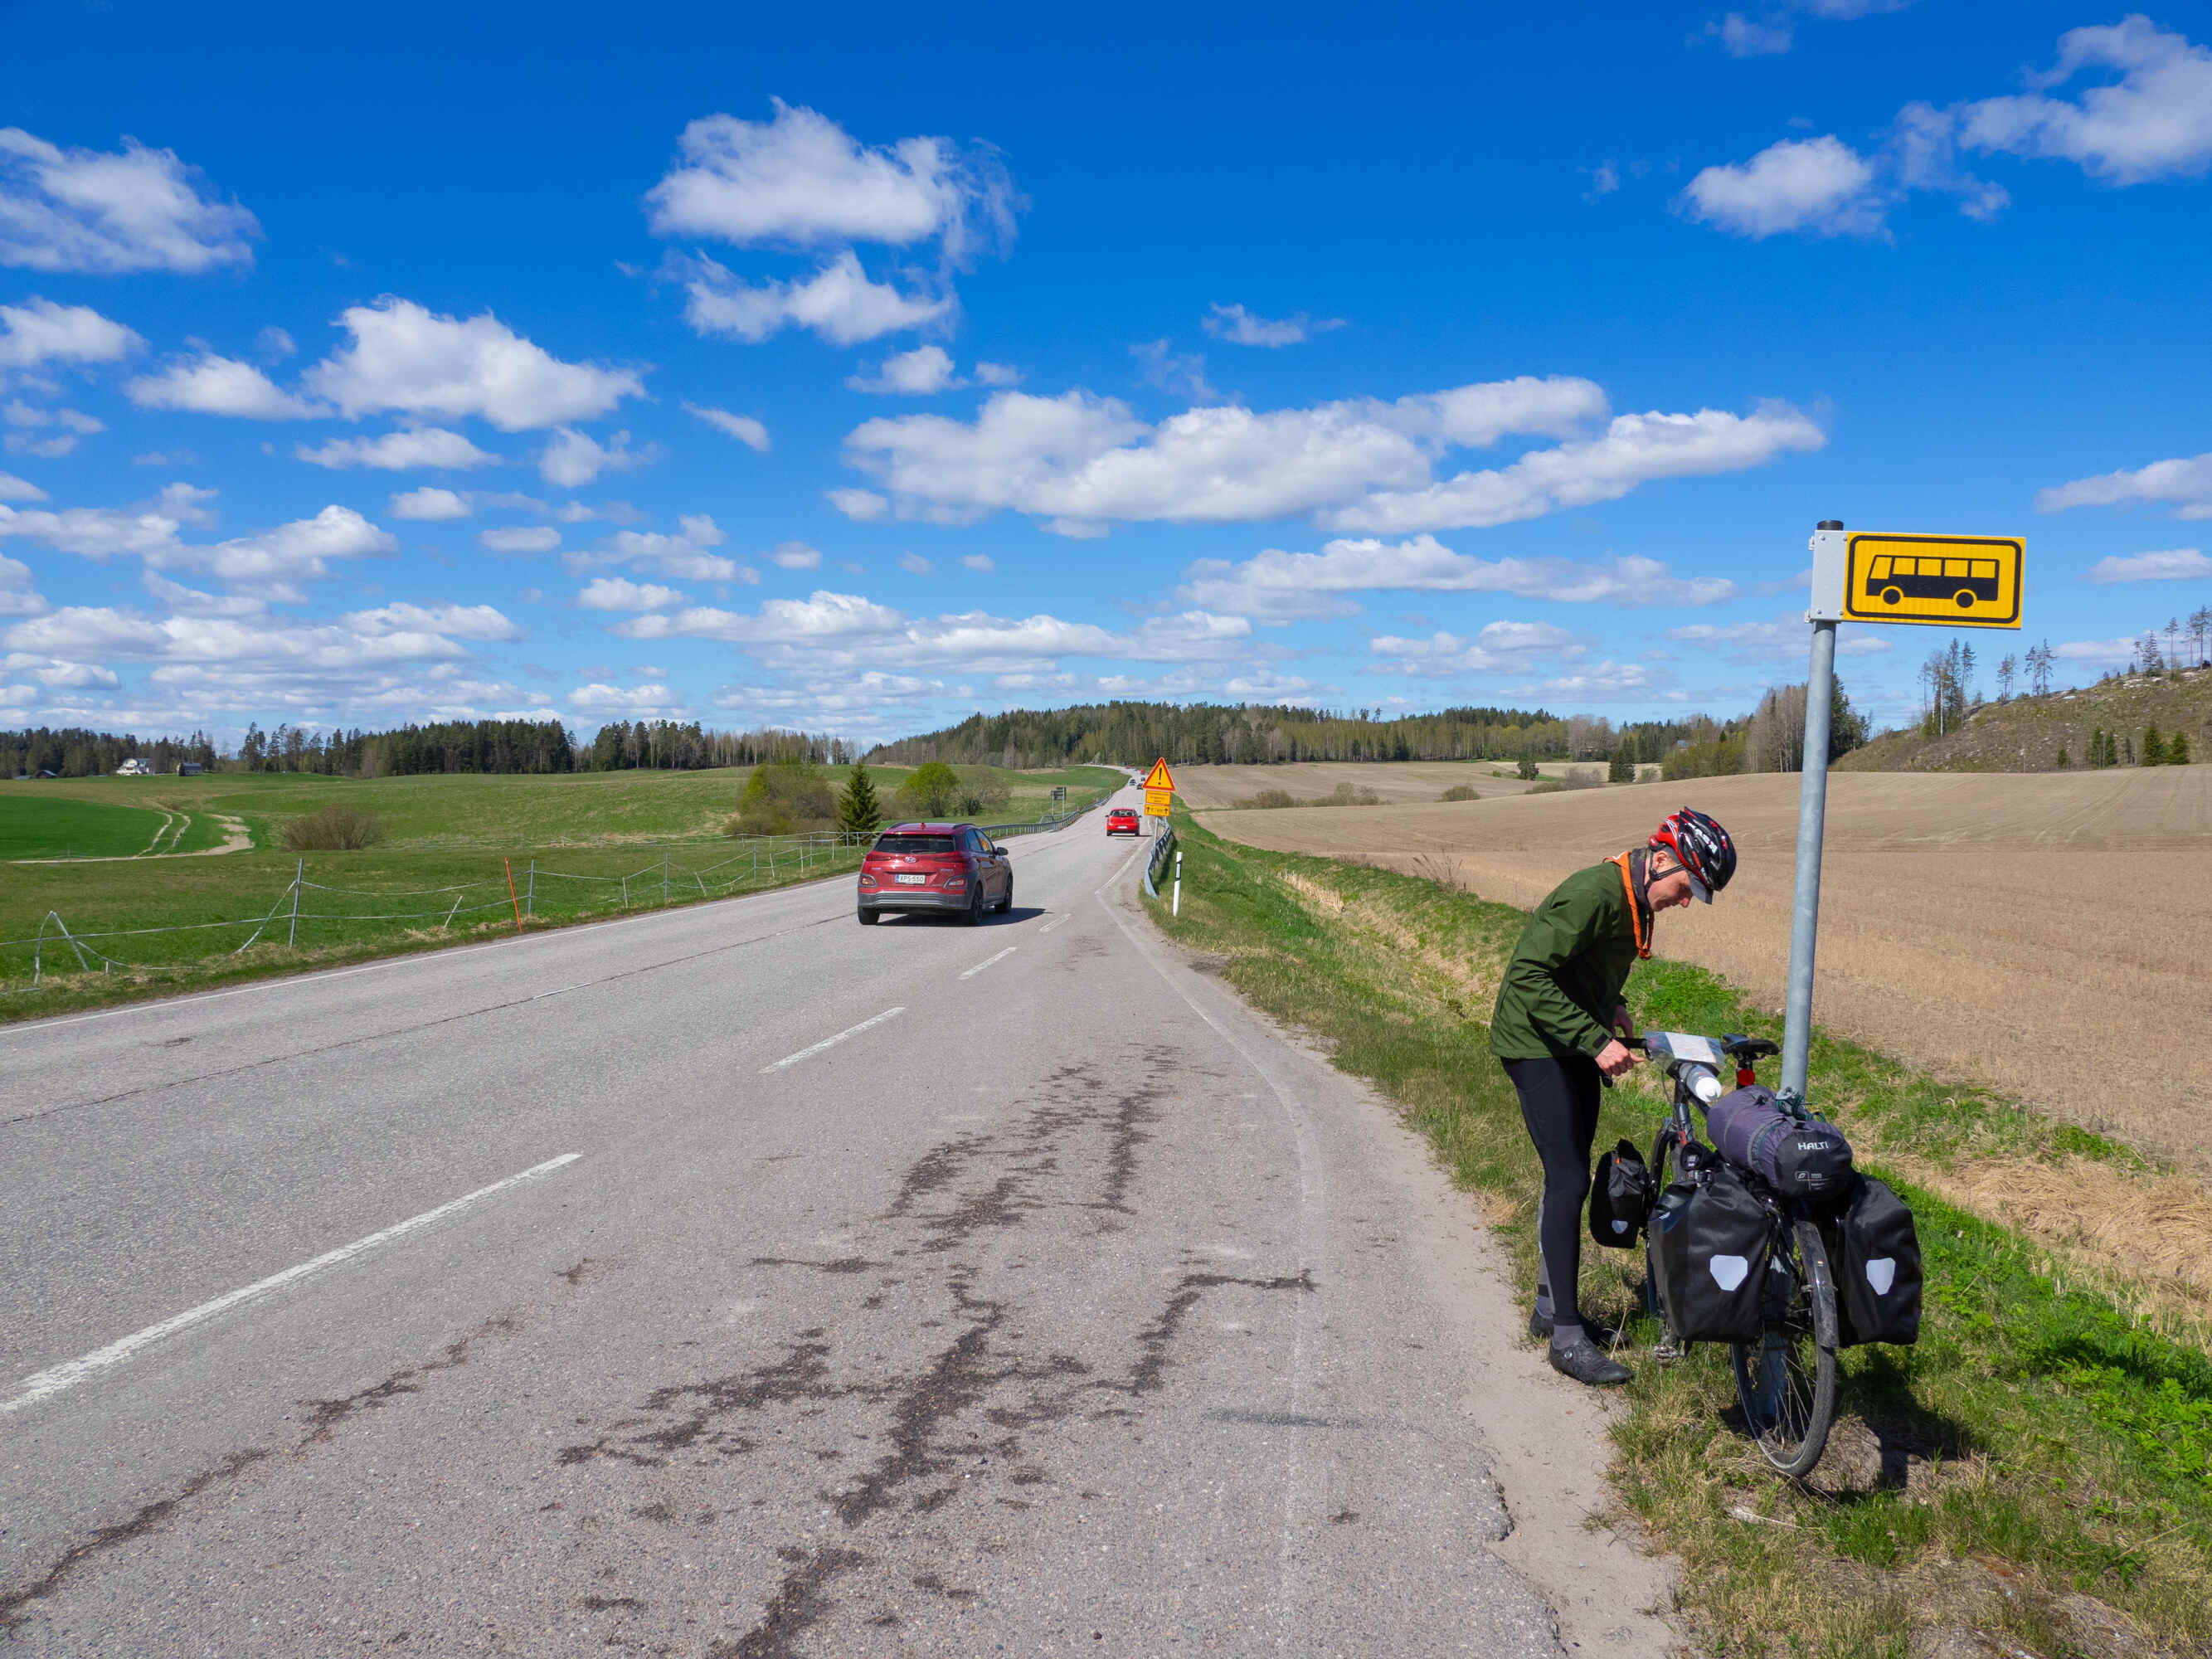
\includegraphics[width=0.90\linewidth]{assets/pyörävaellus8}
	\captionof{figure}{Matka jatkui hyvässä säässää}
\end{center}
\end{Figure}
\begin{Figure}
\begin{center}
	\noindent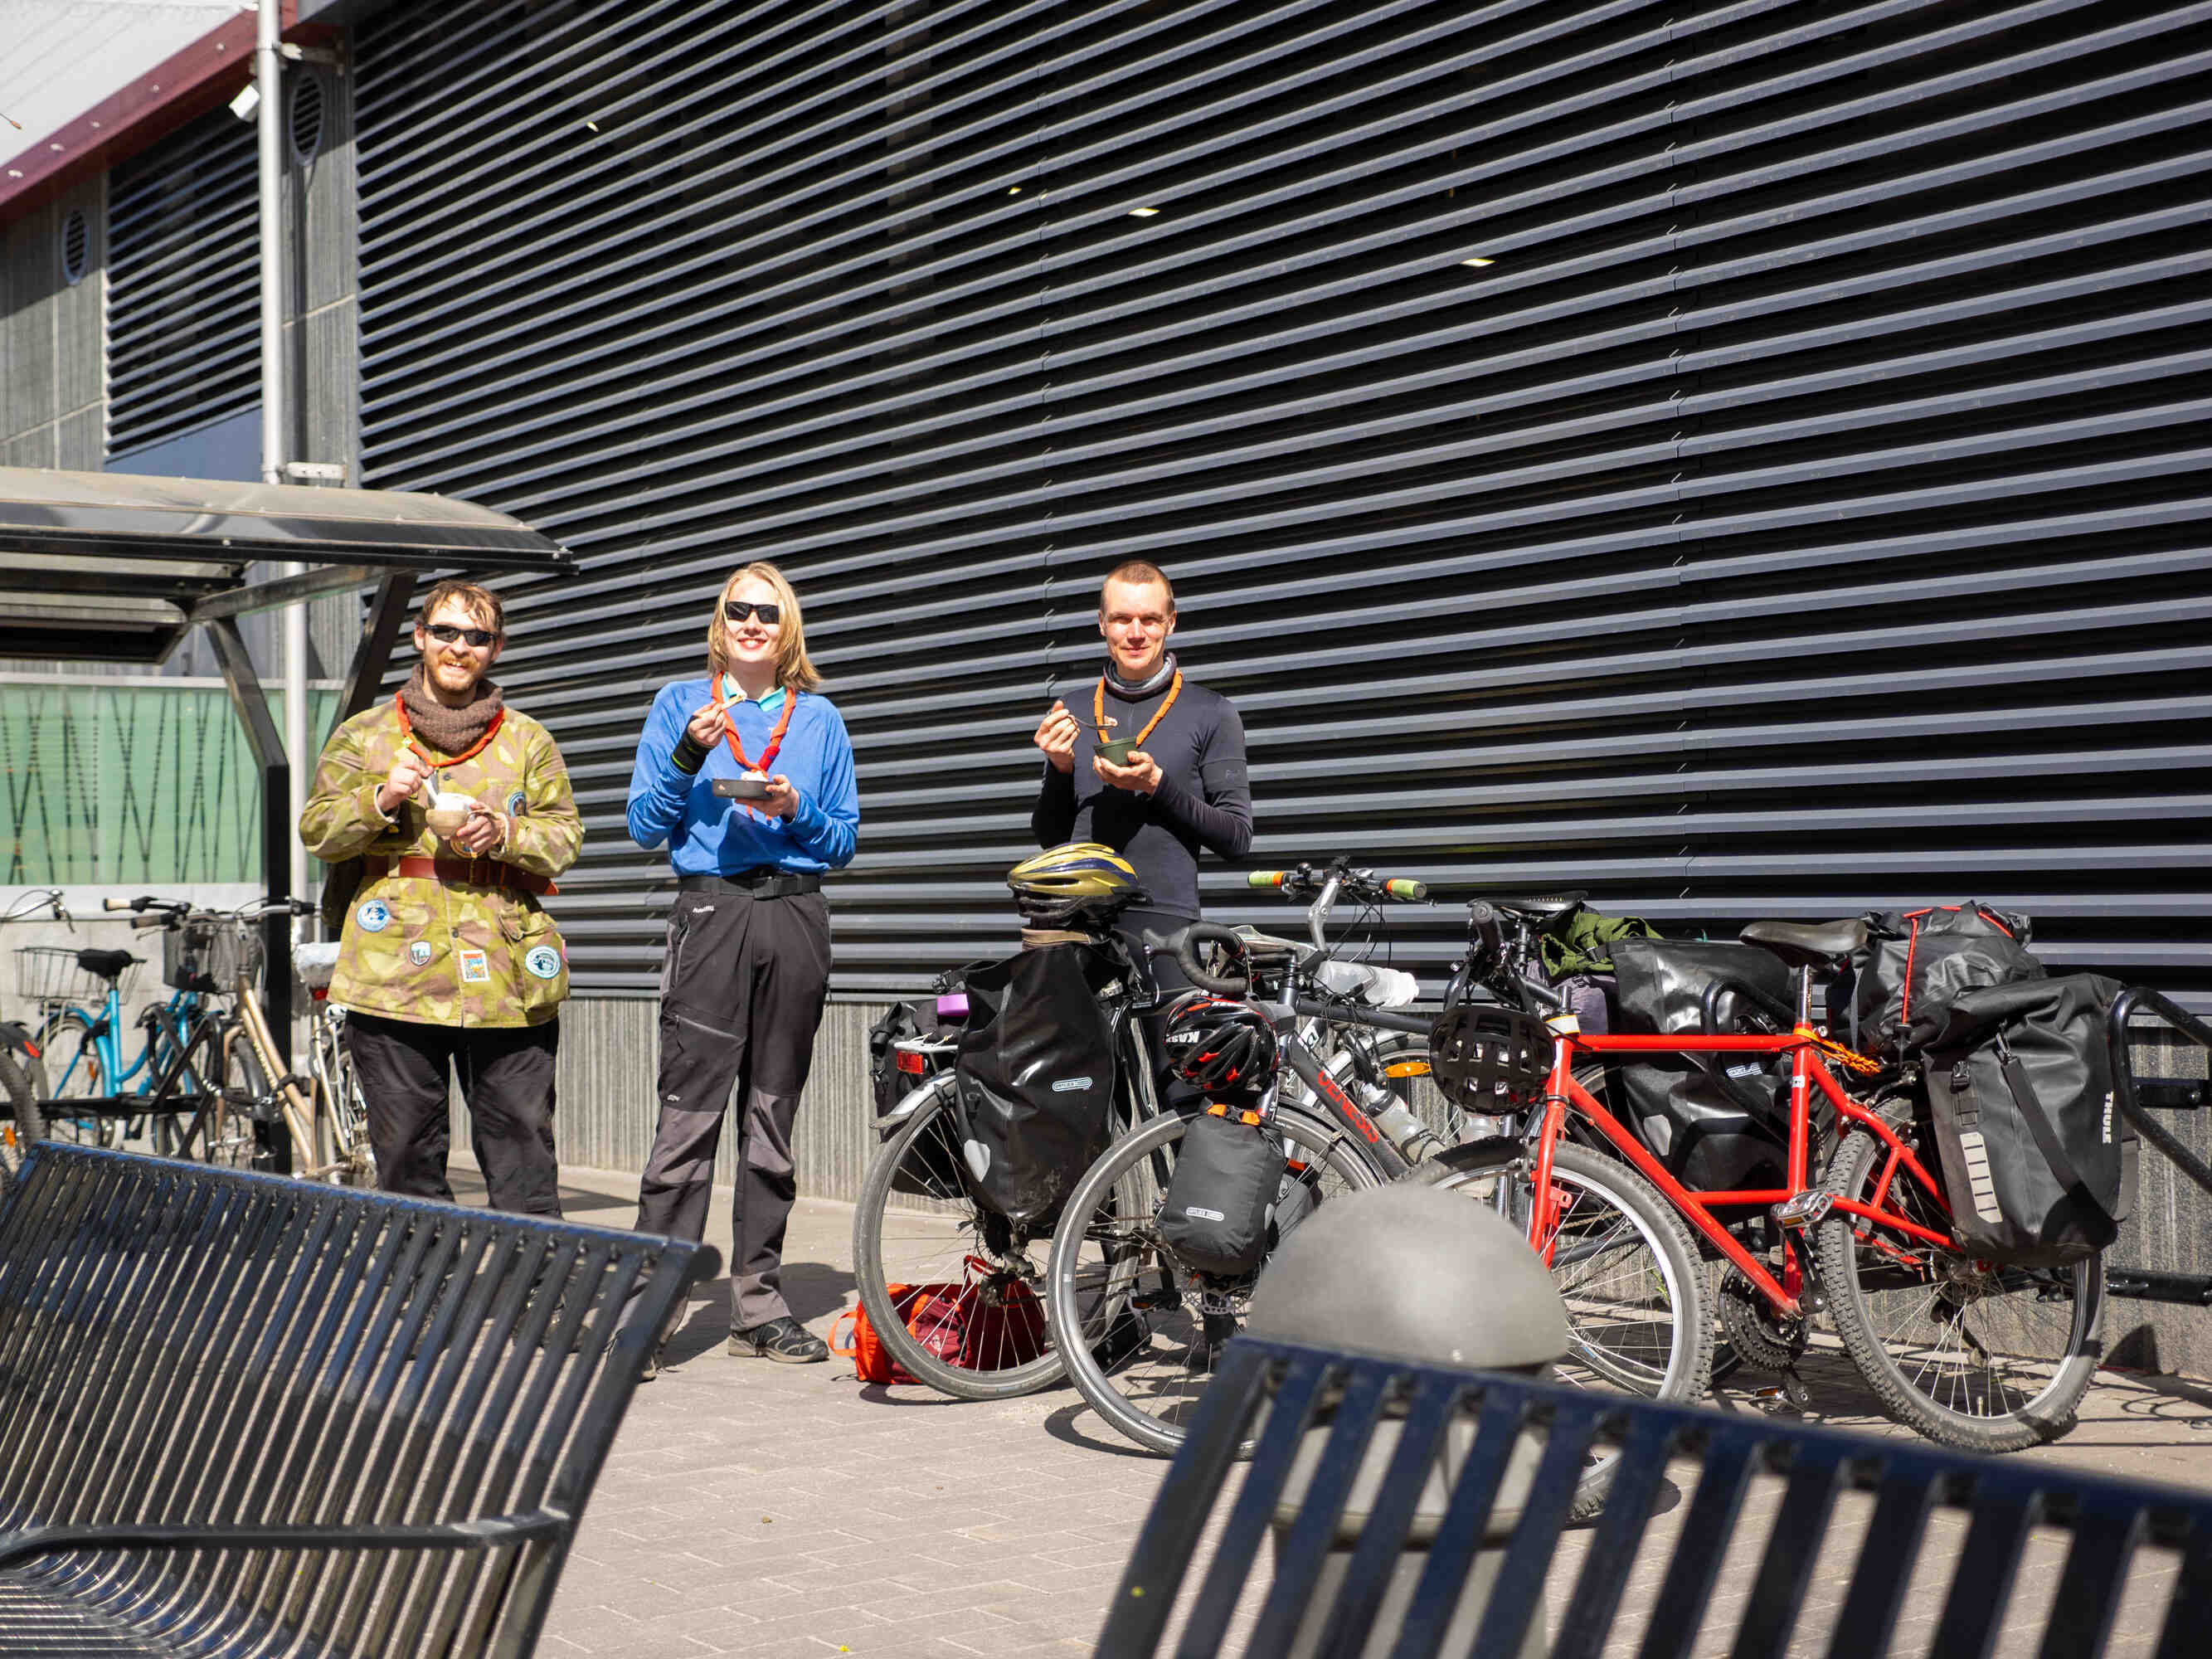
\includegraphics[width=0.90\linewidth]{assets/pyörävaellus9}
	\captionof{figure}{Lohjalla syötiin vaelluksen toinen jäätelö.}
\end{center}
\end{Figure}


\begin{Figure}
\begin{center}
	\begin{multicols}{2}
		\begin{center}
			\noindent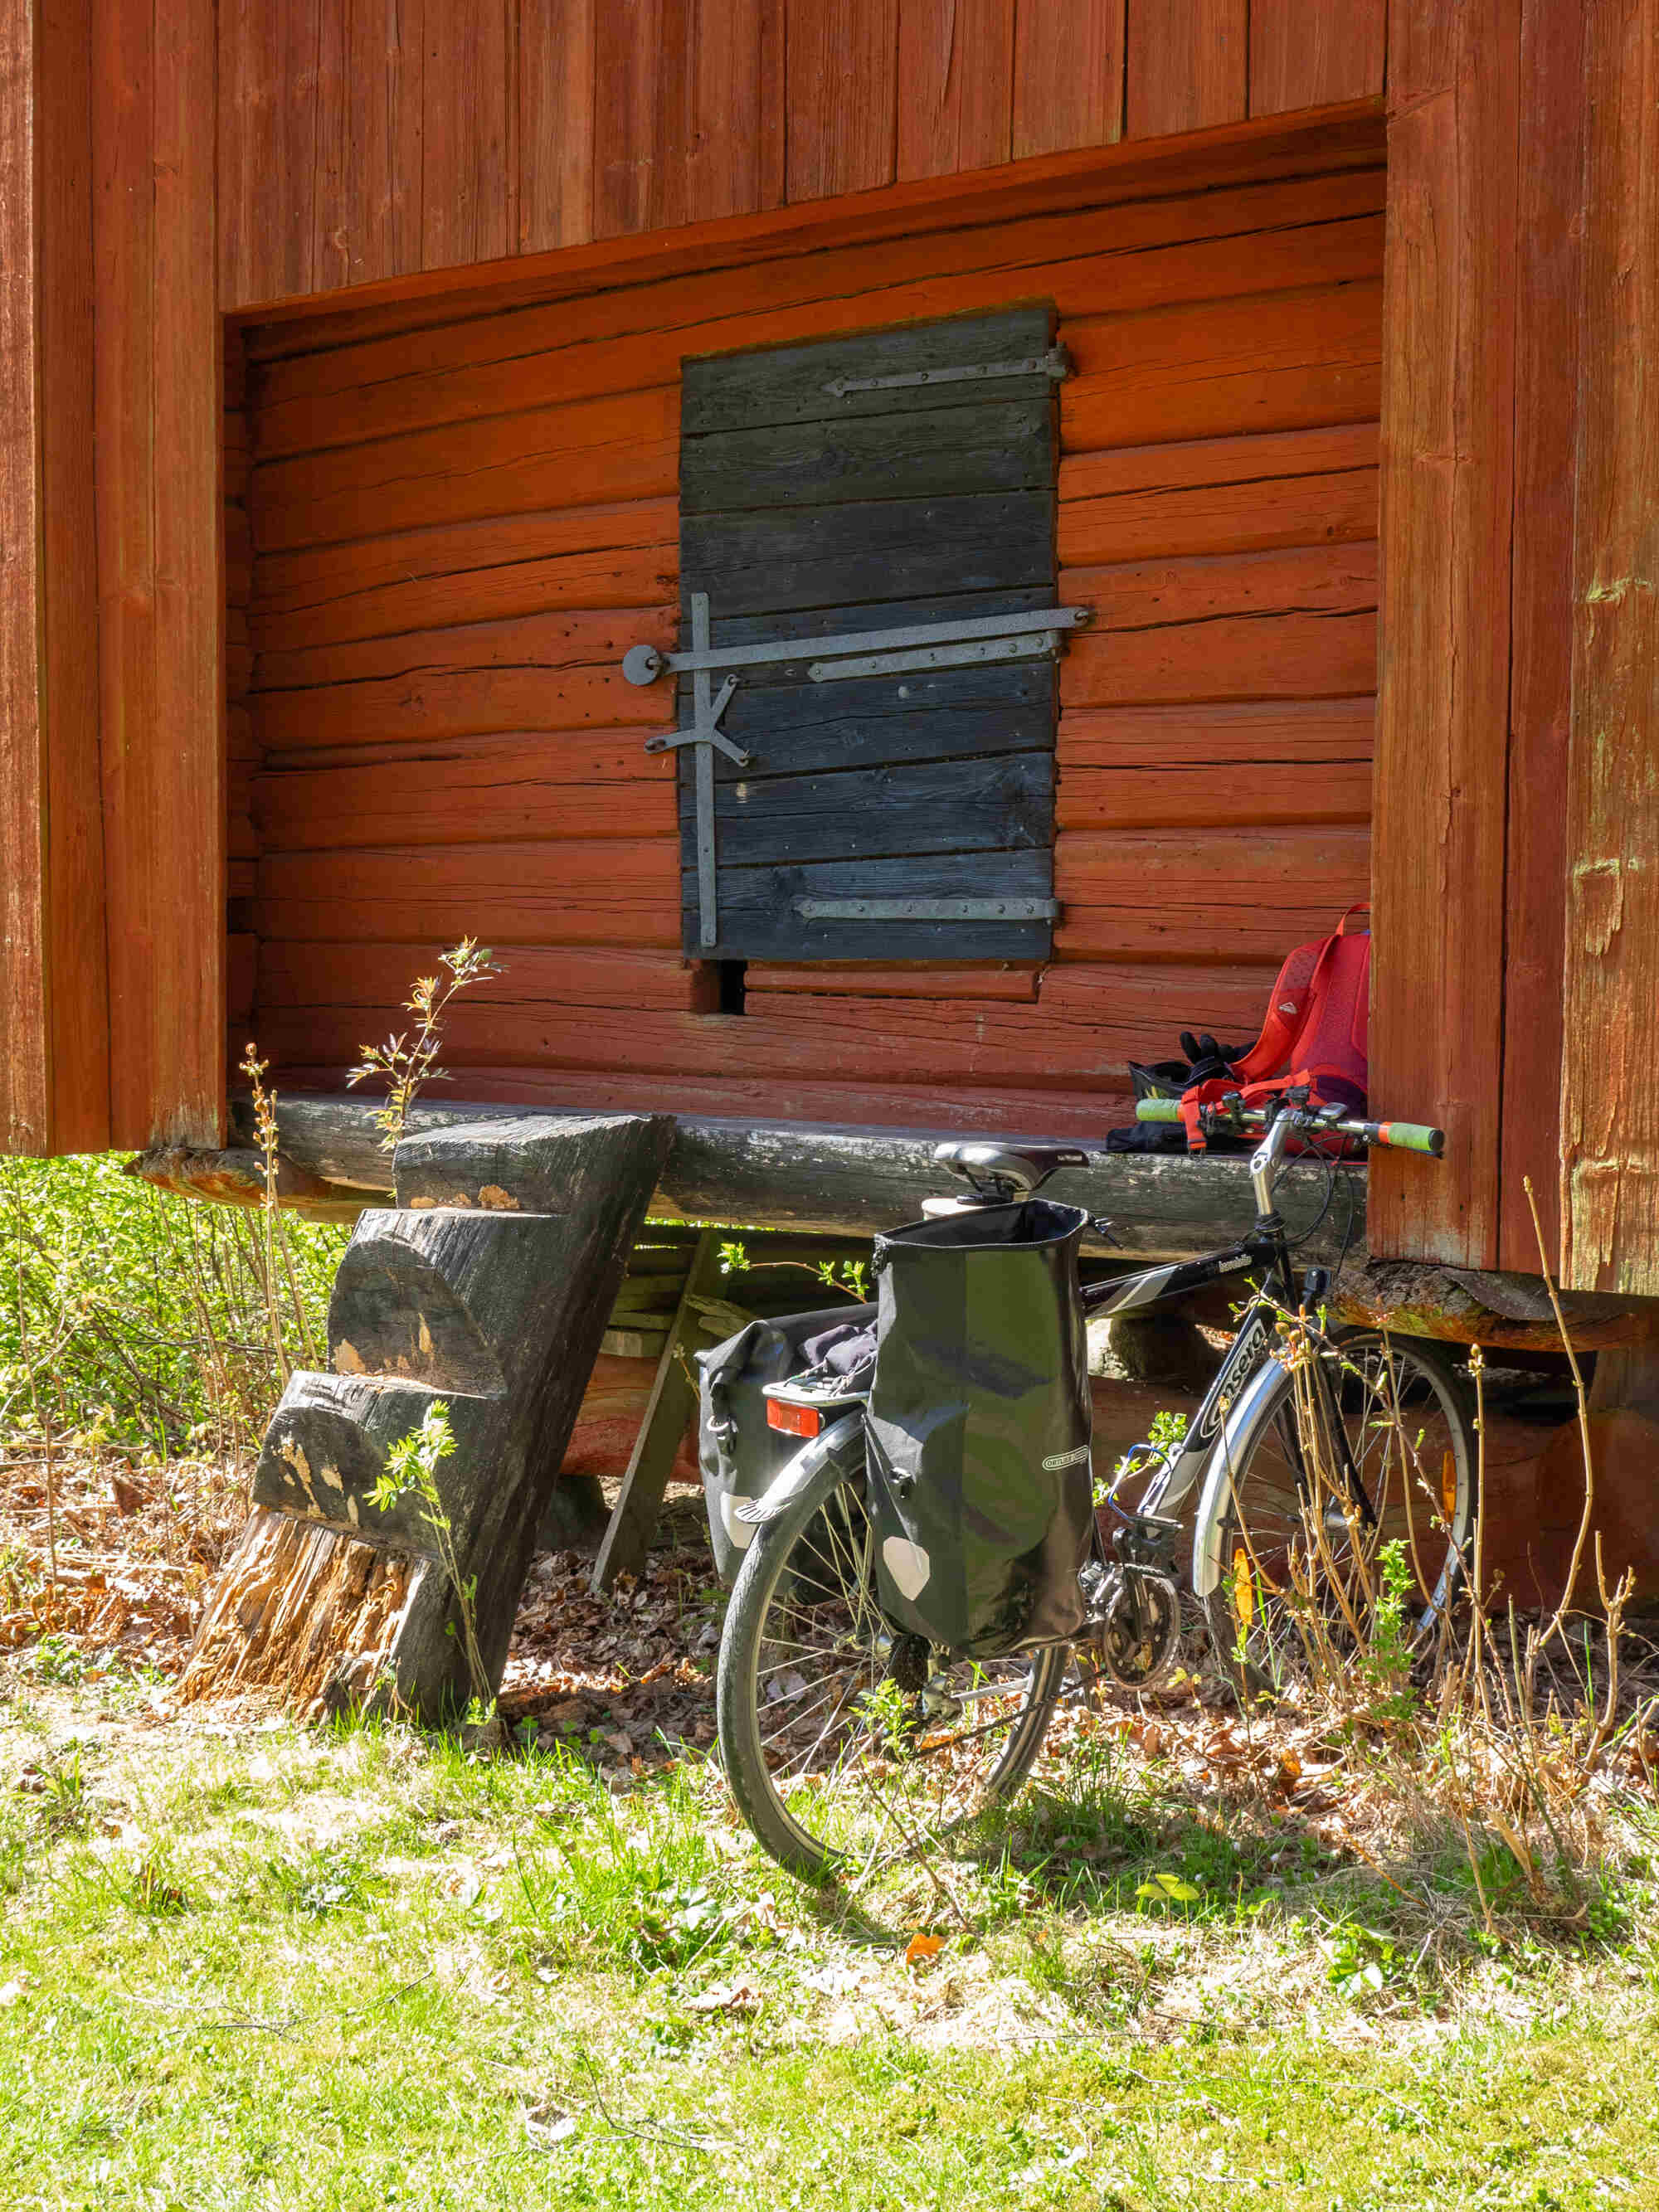
\includegraphics[width=1.05\linewidth]{assets/pyörävaellus10}
			\noindent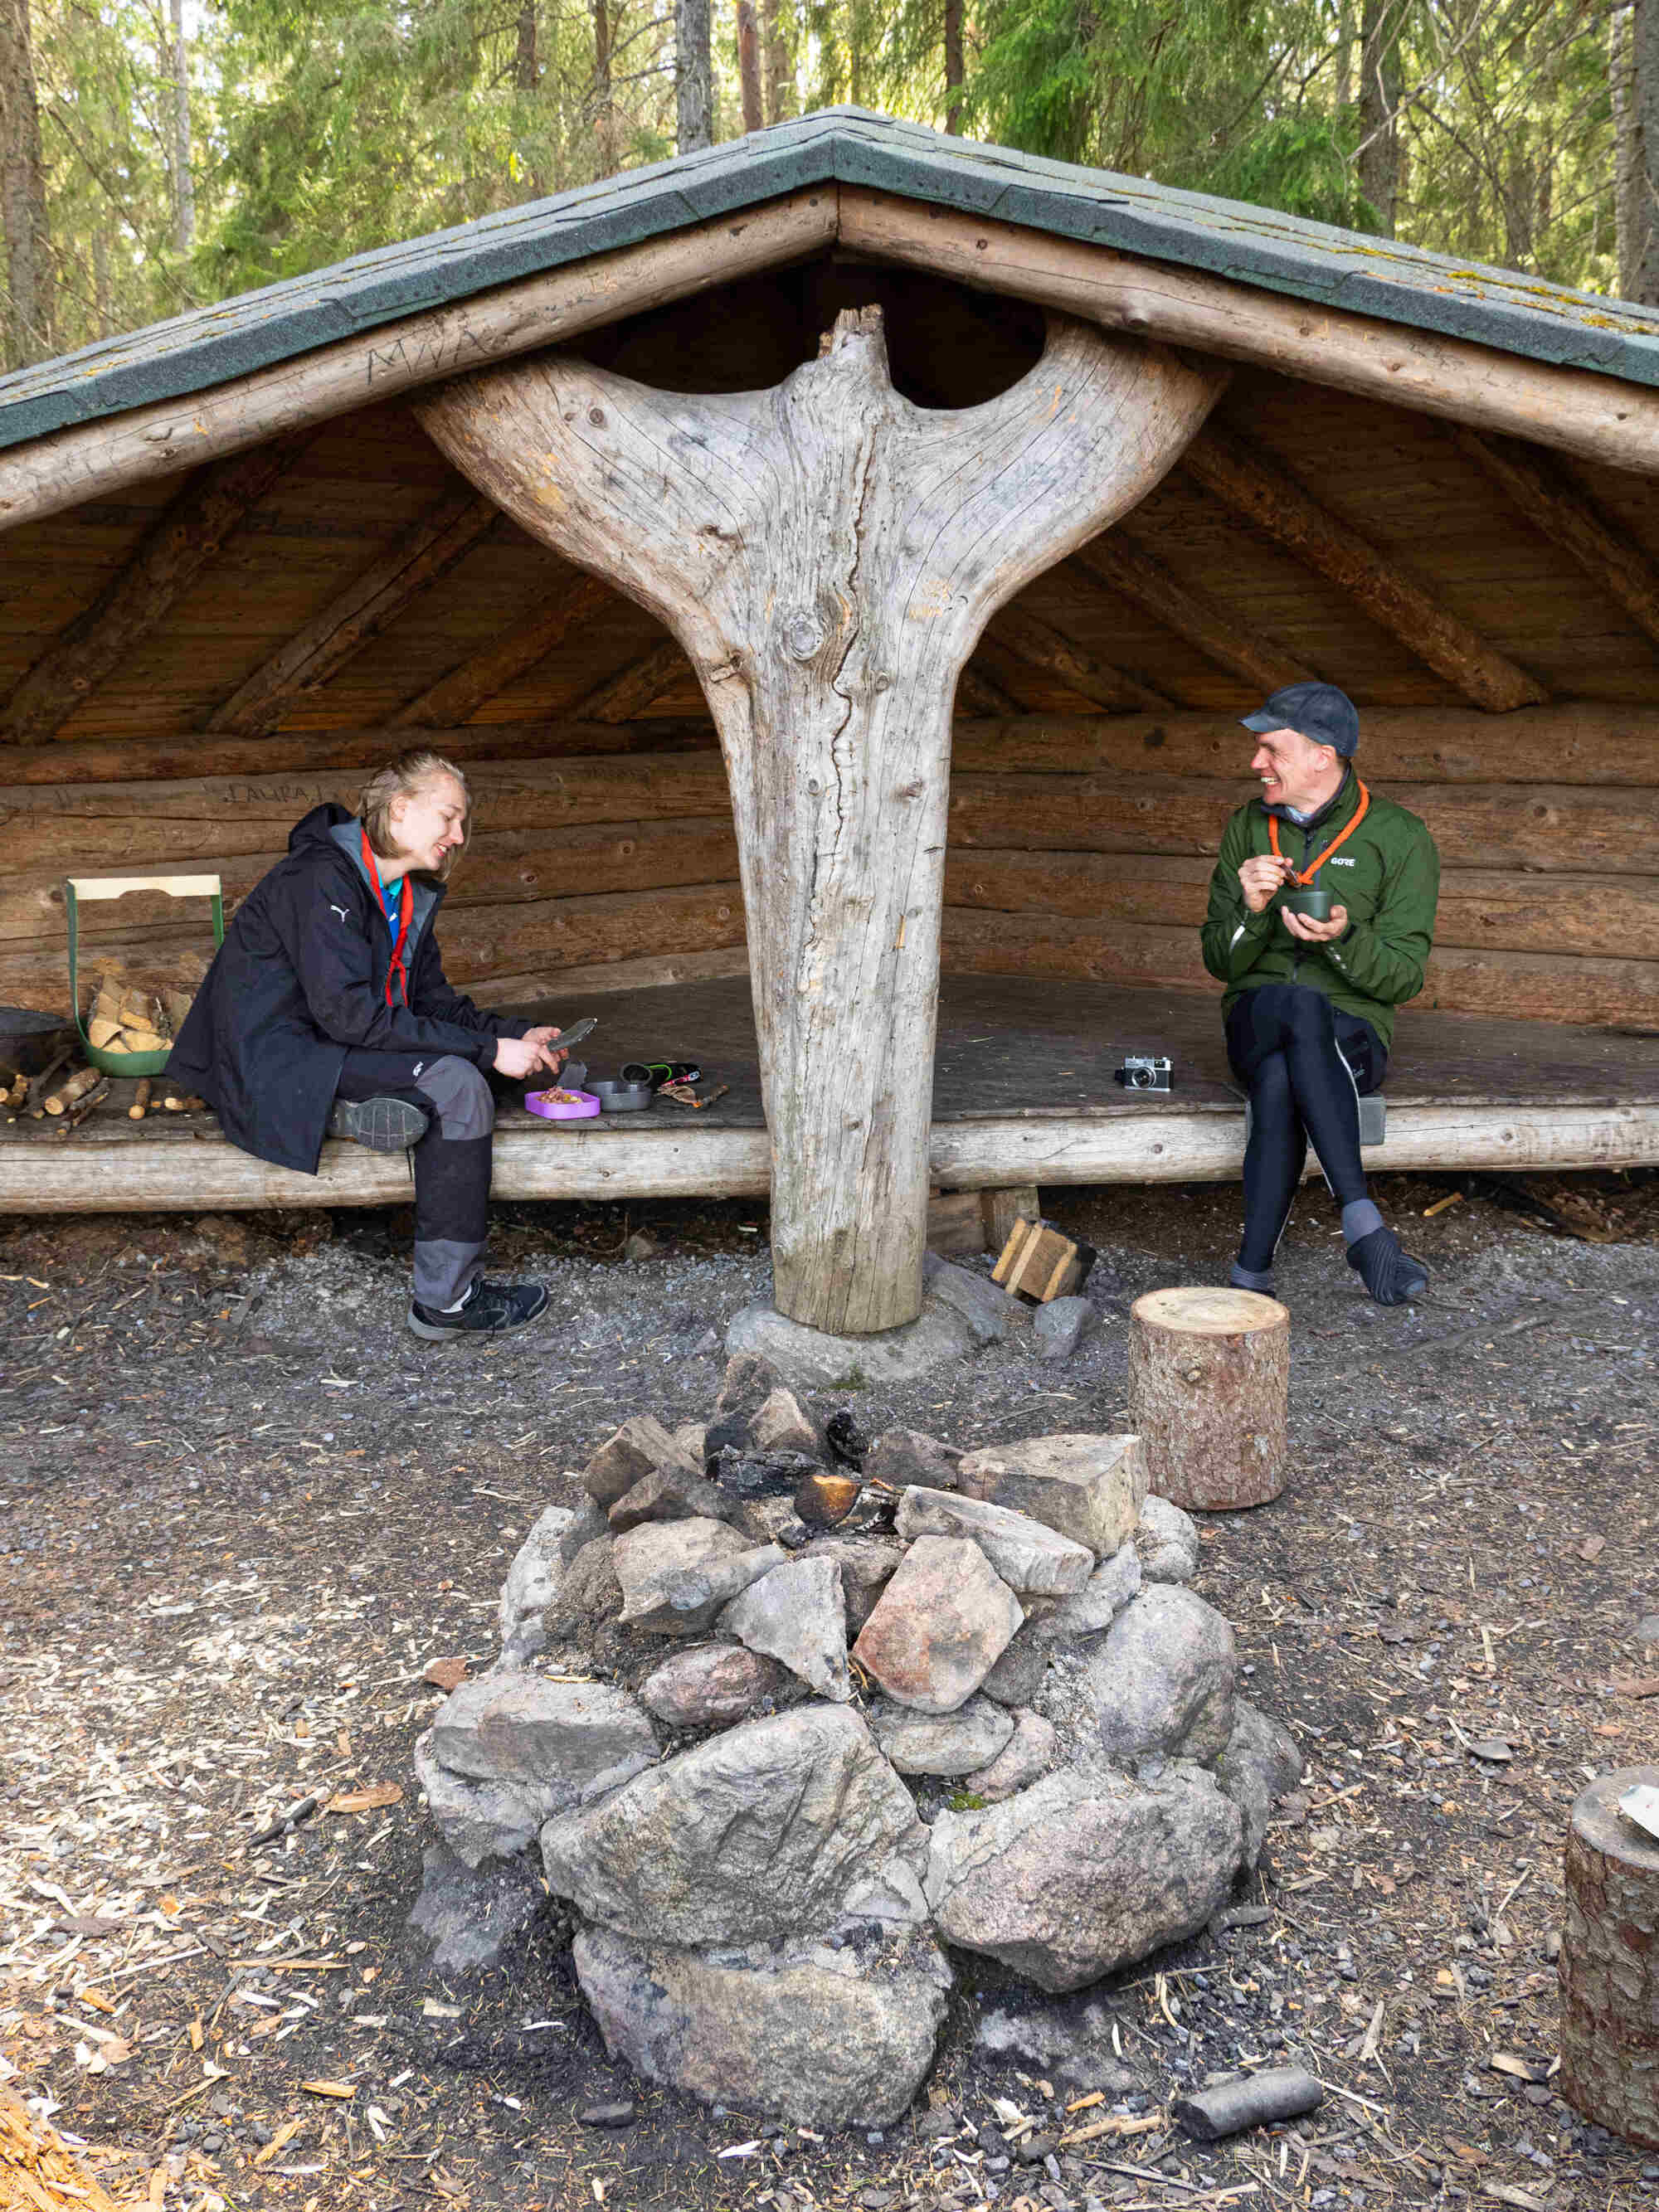
\includegraphics[width=1.05\linewidth]{assets/pyörävaellus13}
		\end{center}
		\columnbreak
		\begin{center}
			\noindent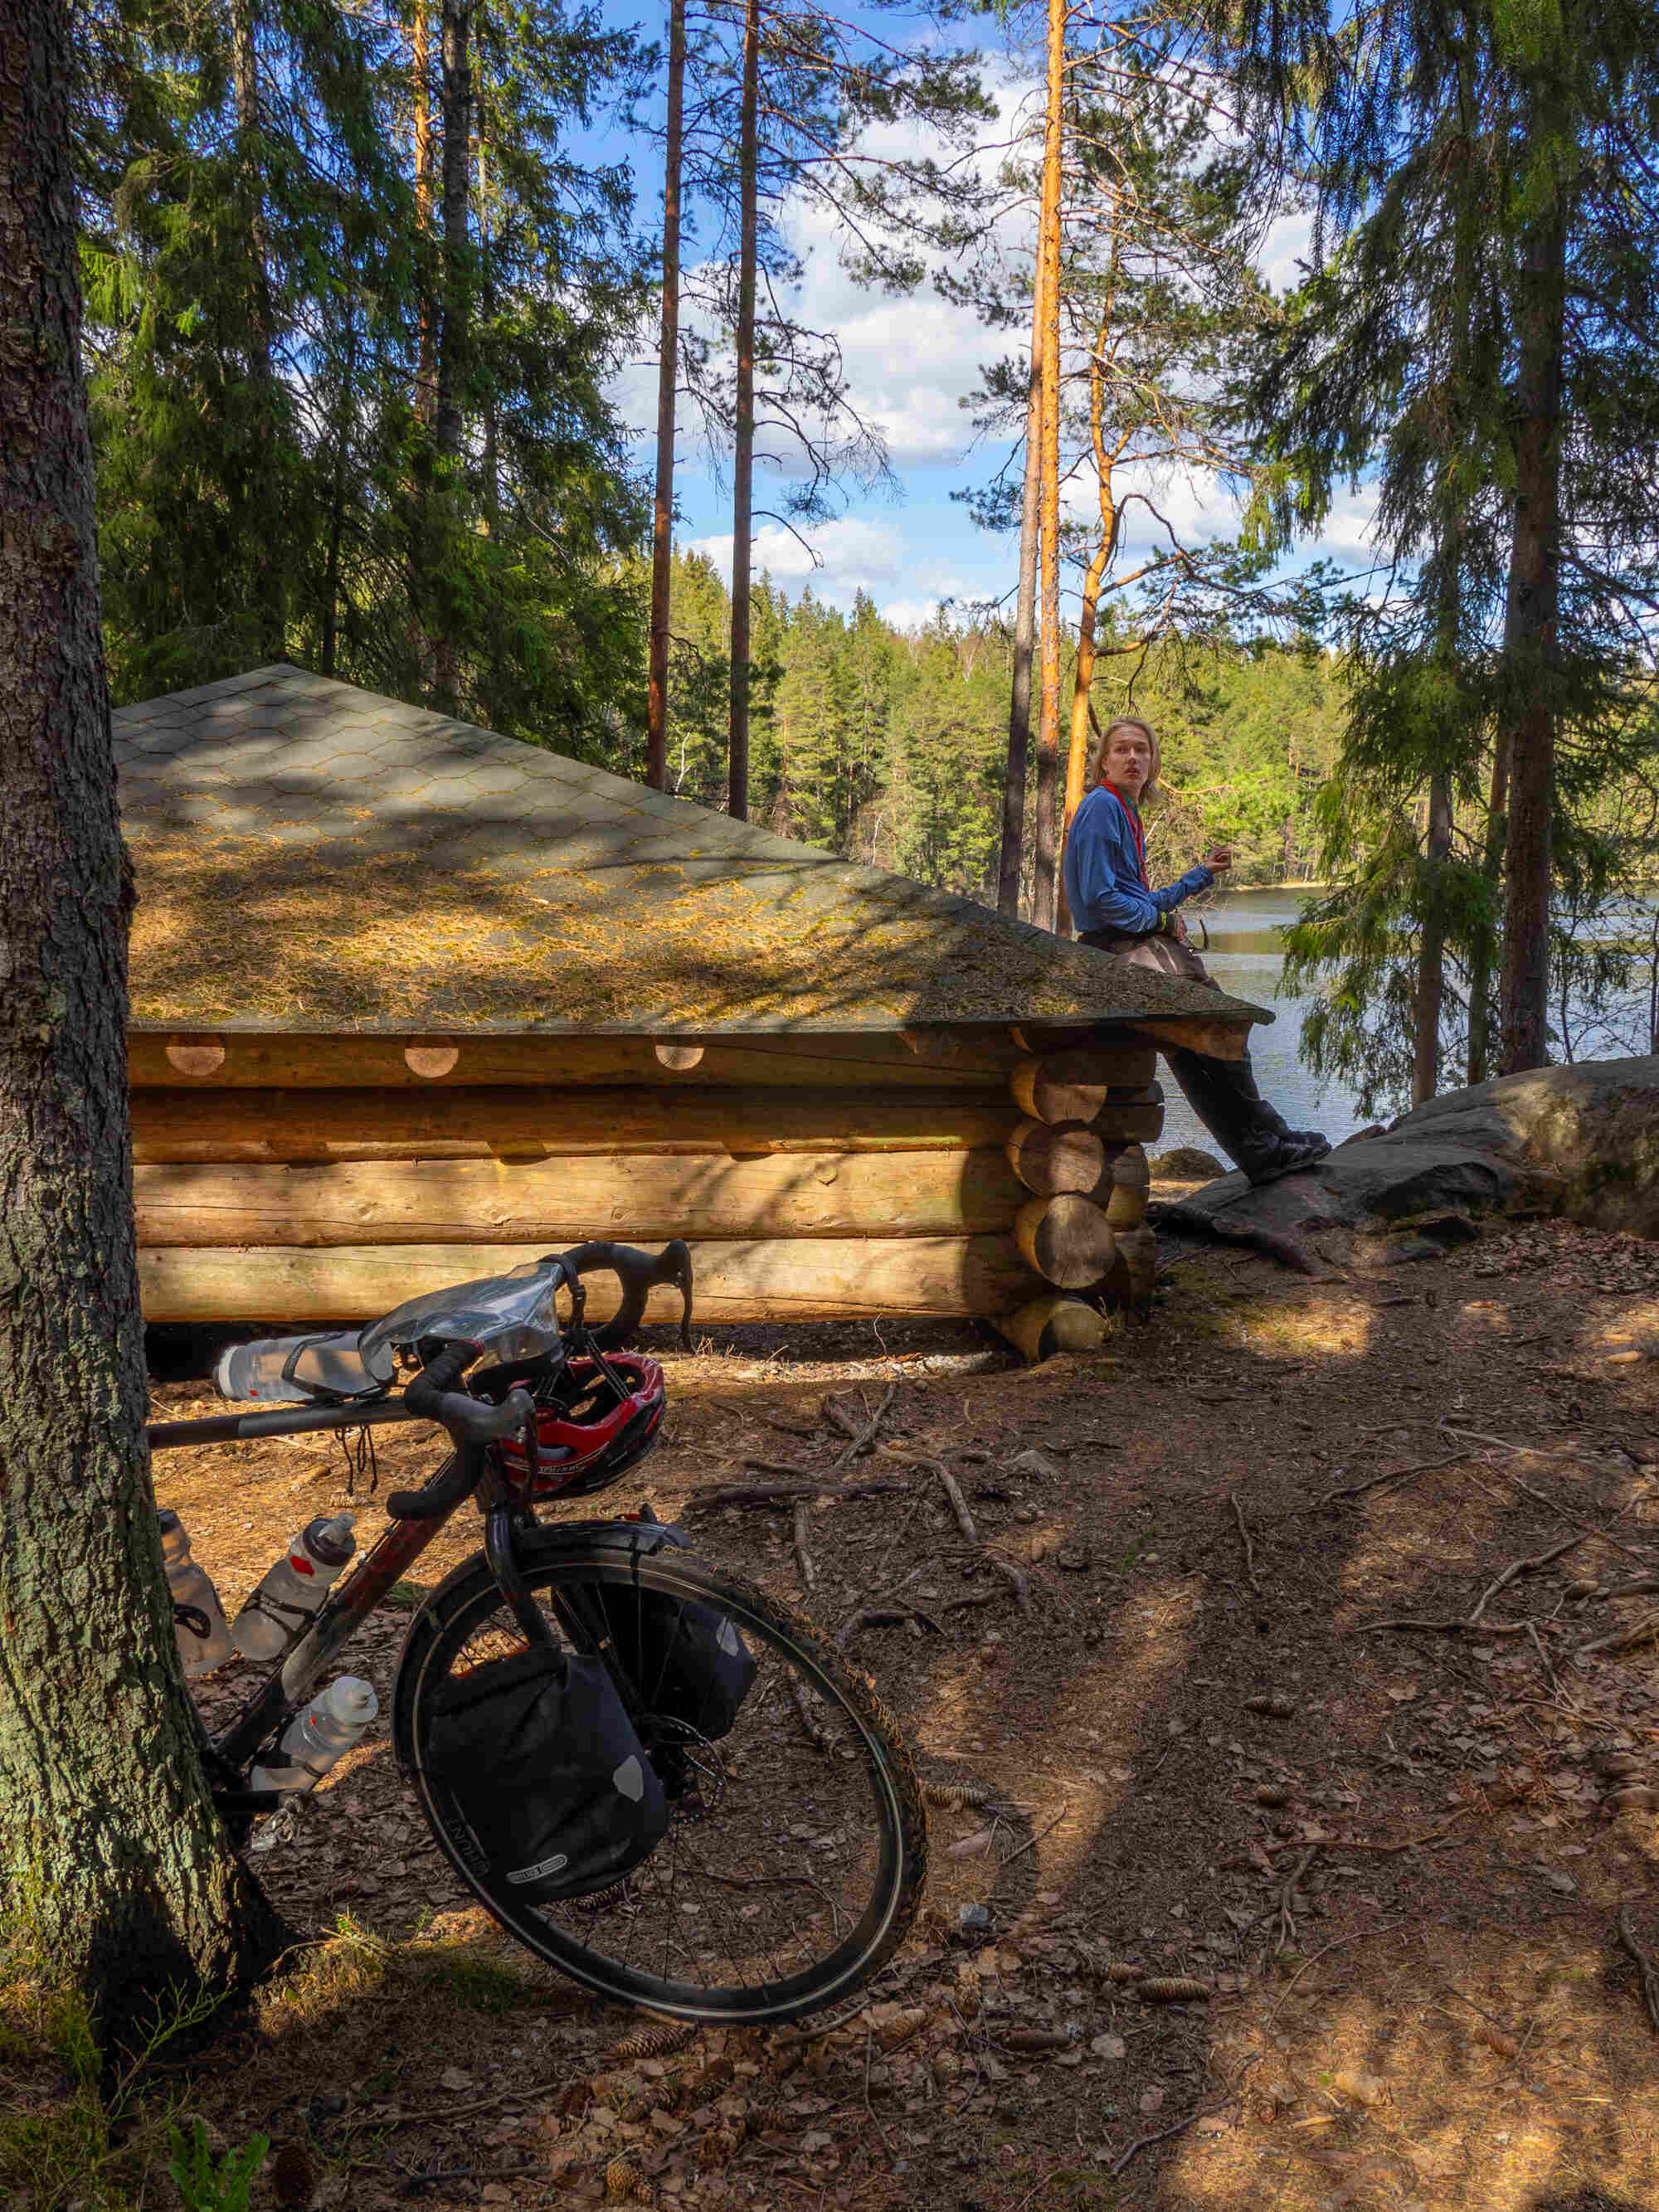
\includegraphics[width=1.05\linewidth]{assets/pyörävaellus11}
			\noindent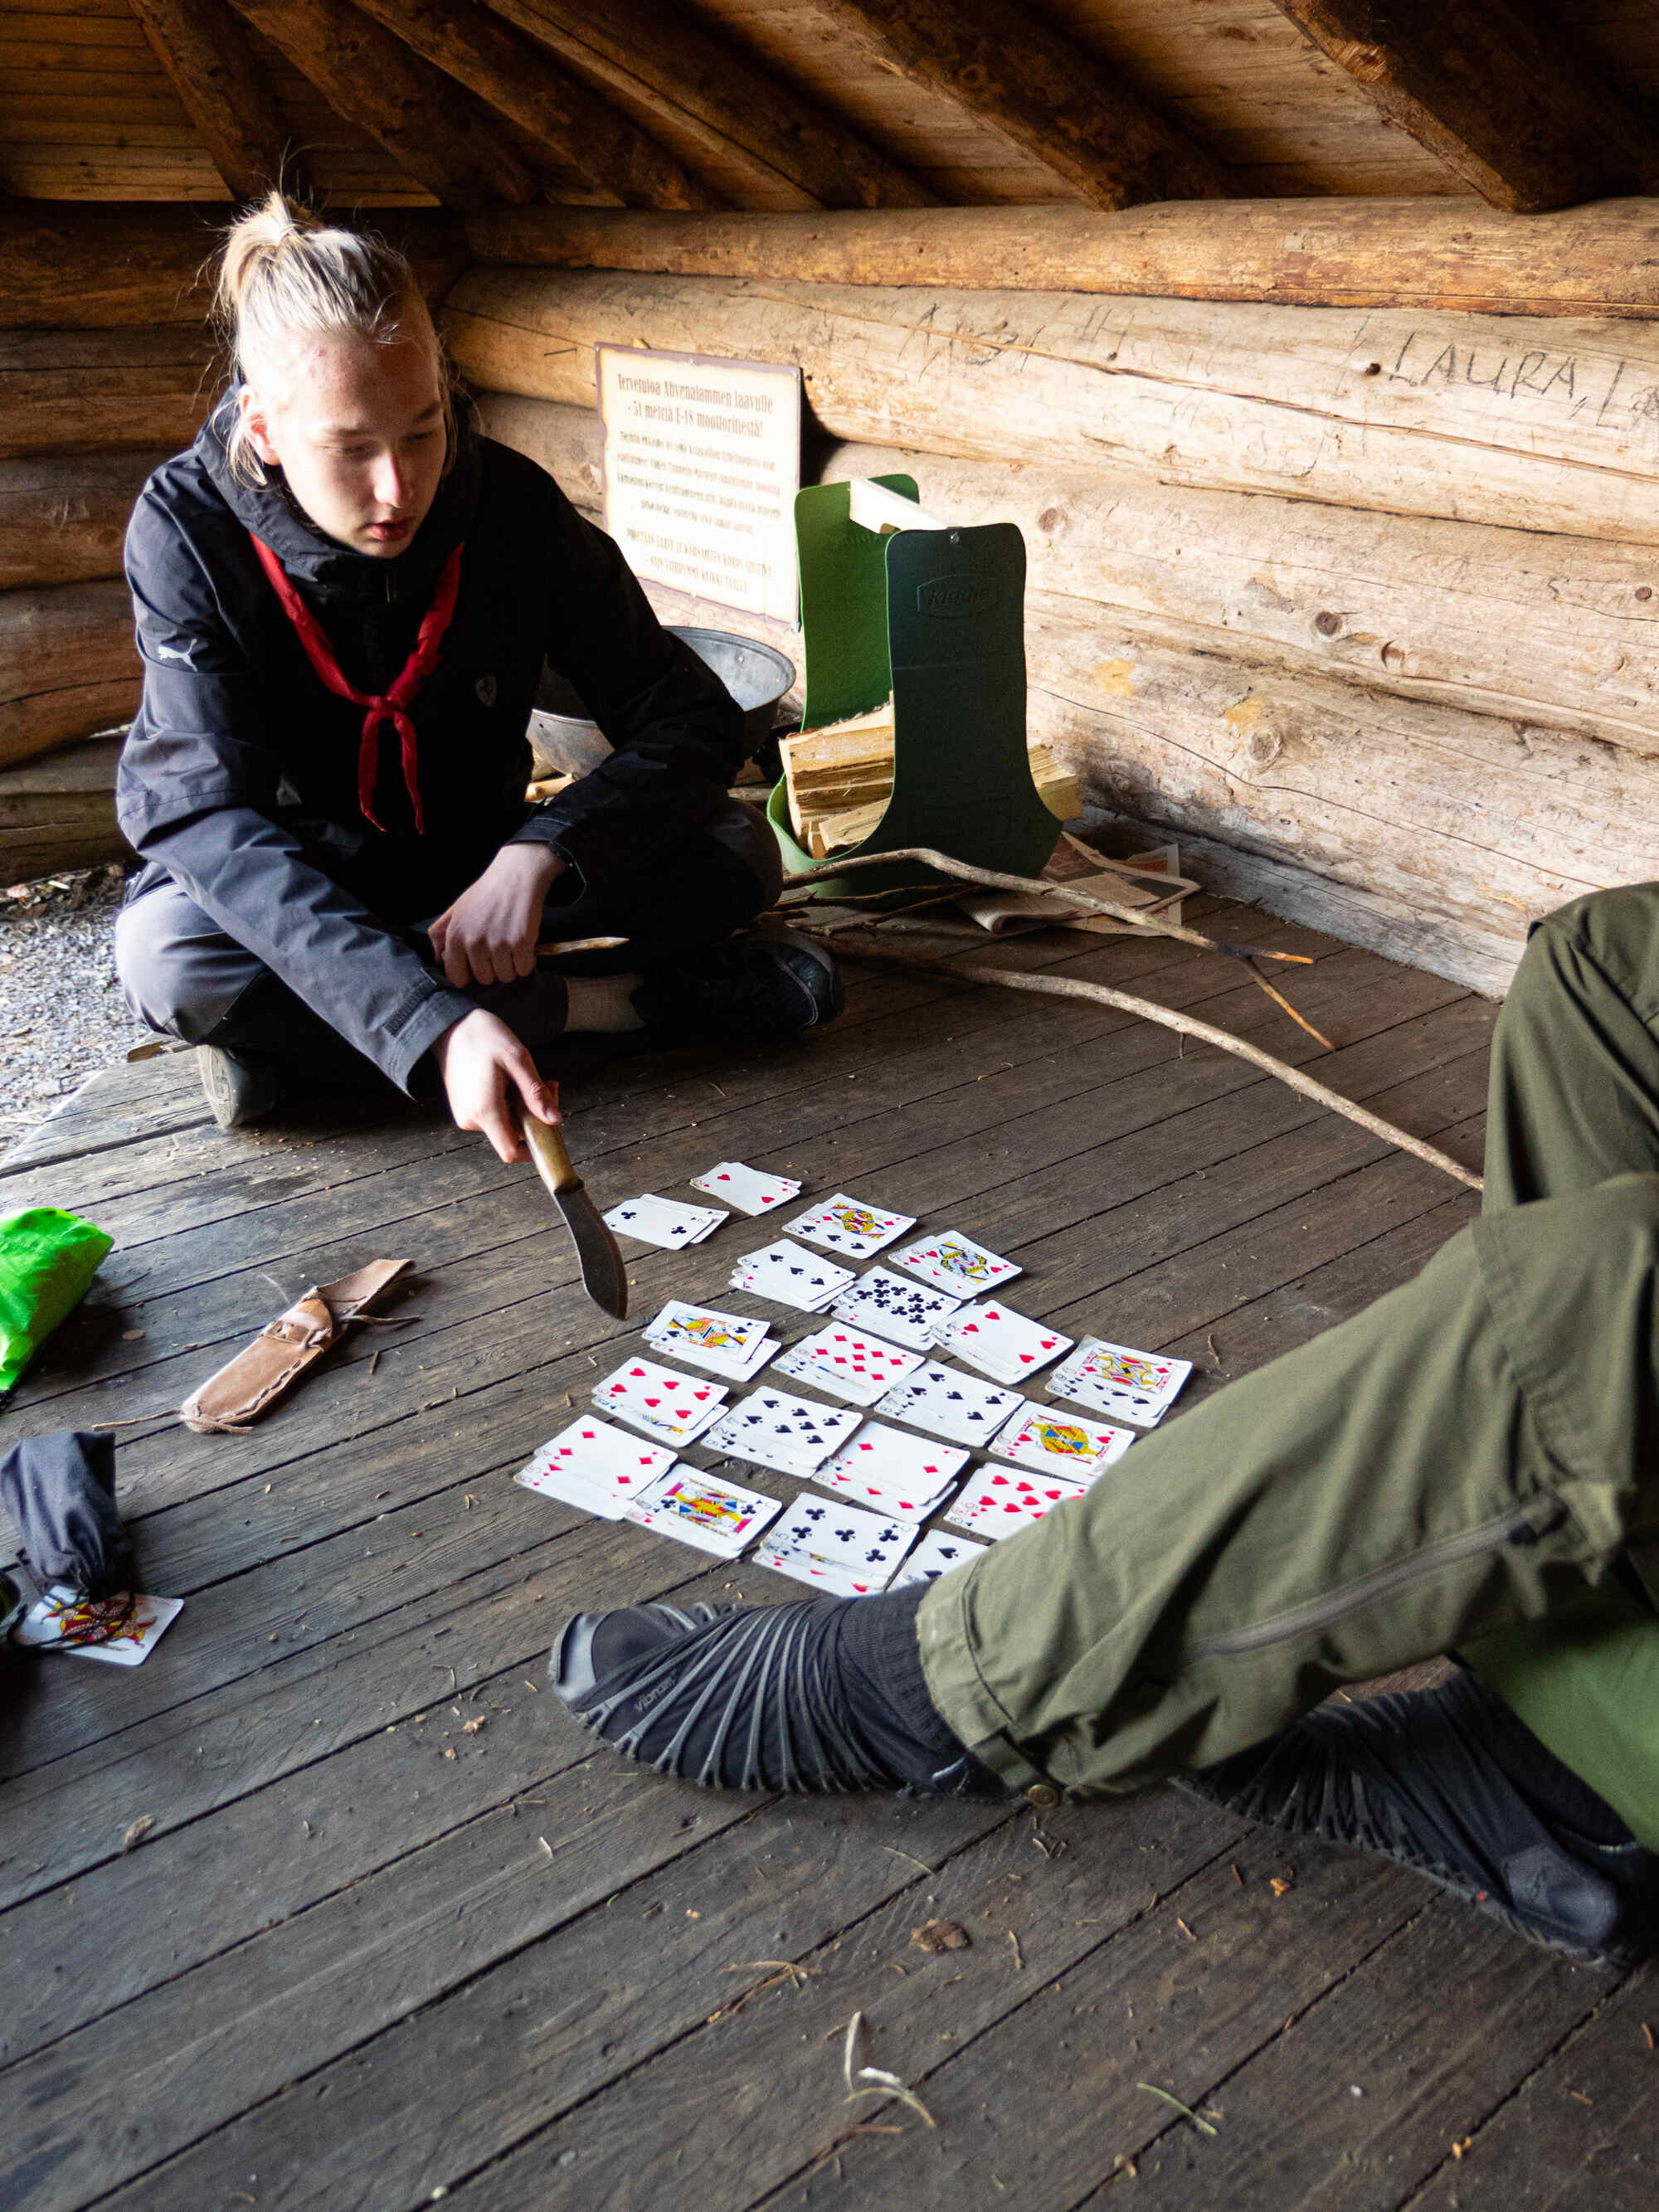
\includegraphics[width=1.05\linewidth]{assets/pyörävaellus15}
		\end{center}
	\end{multicols}
	\vspace*{-0.32cm}
	\captionof{figure}{Ja 47km jälkeen, löytyi meidän seuraava
	yöpymispaikka: Ahvenalampi, Lohja}
\end{center}
\end{Figure}


\begin{Figure}
	\noindent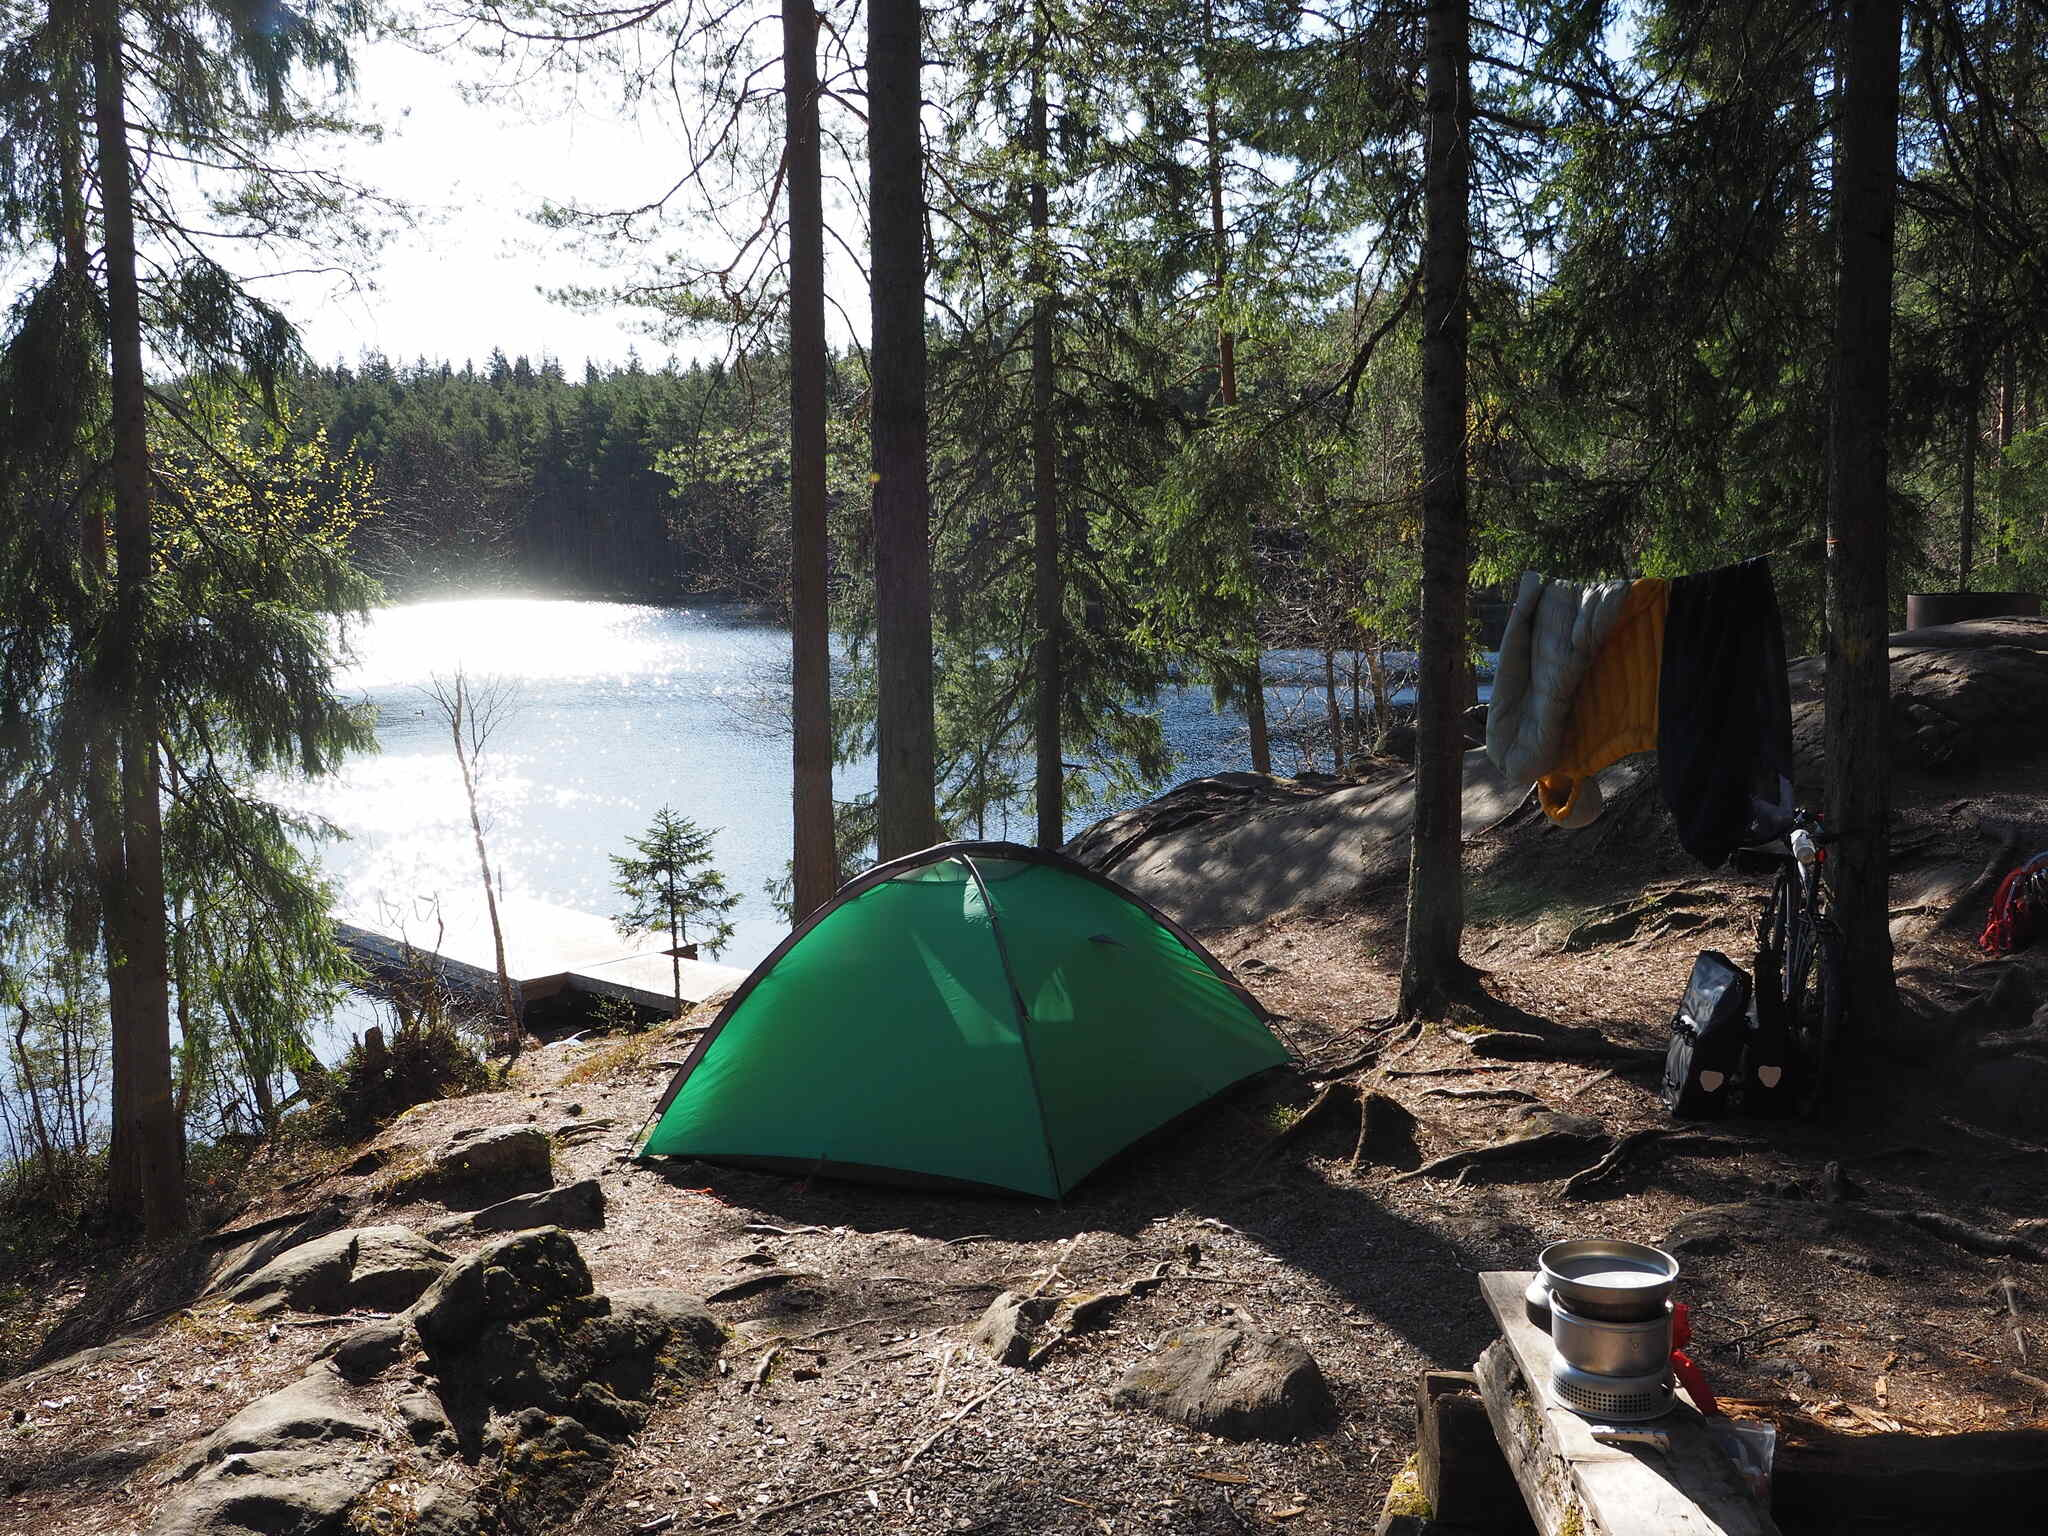
\includegraphics[width=\linewidth]{assets/pyörävaellus16}
	\captionof{figure}{Hauska fakta: nukuimme suoraan päällä
	Helsinki-Turku-moottoritien, joka tässä paikassa kulkee tunnelin läpi}
\end{Figure}

\begin{multicols}{2}
	\begin{center}
		\noindent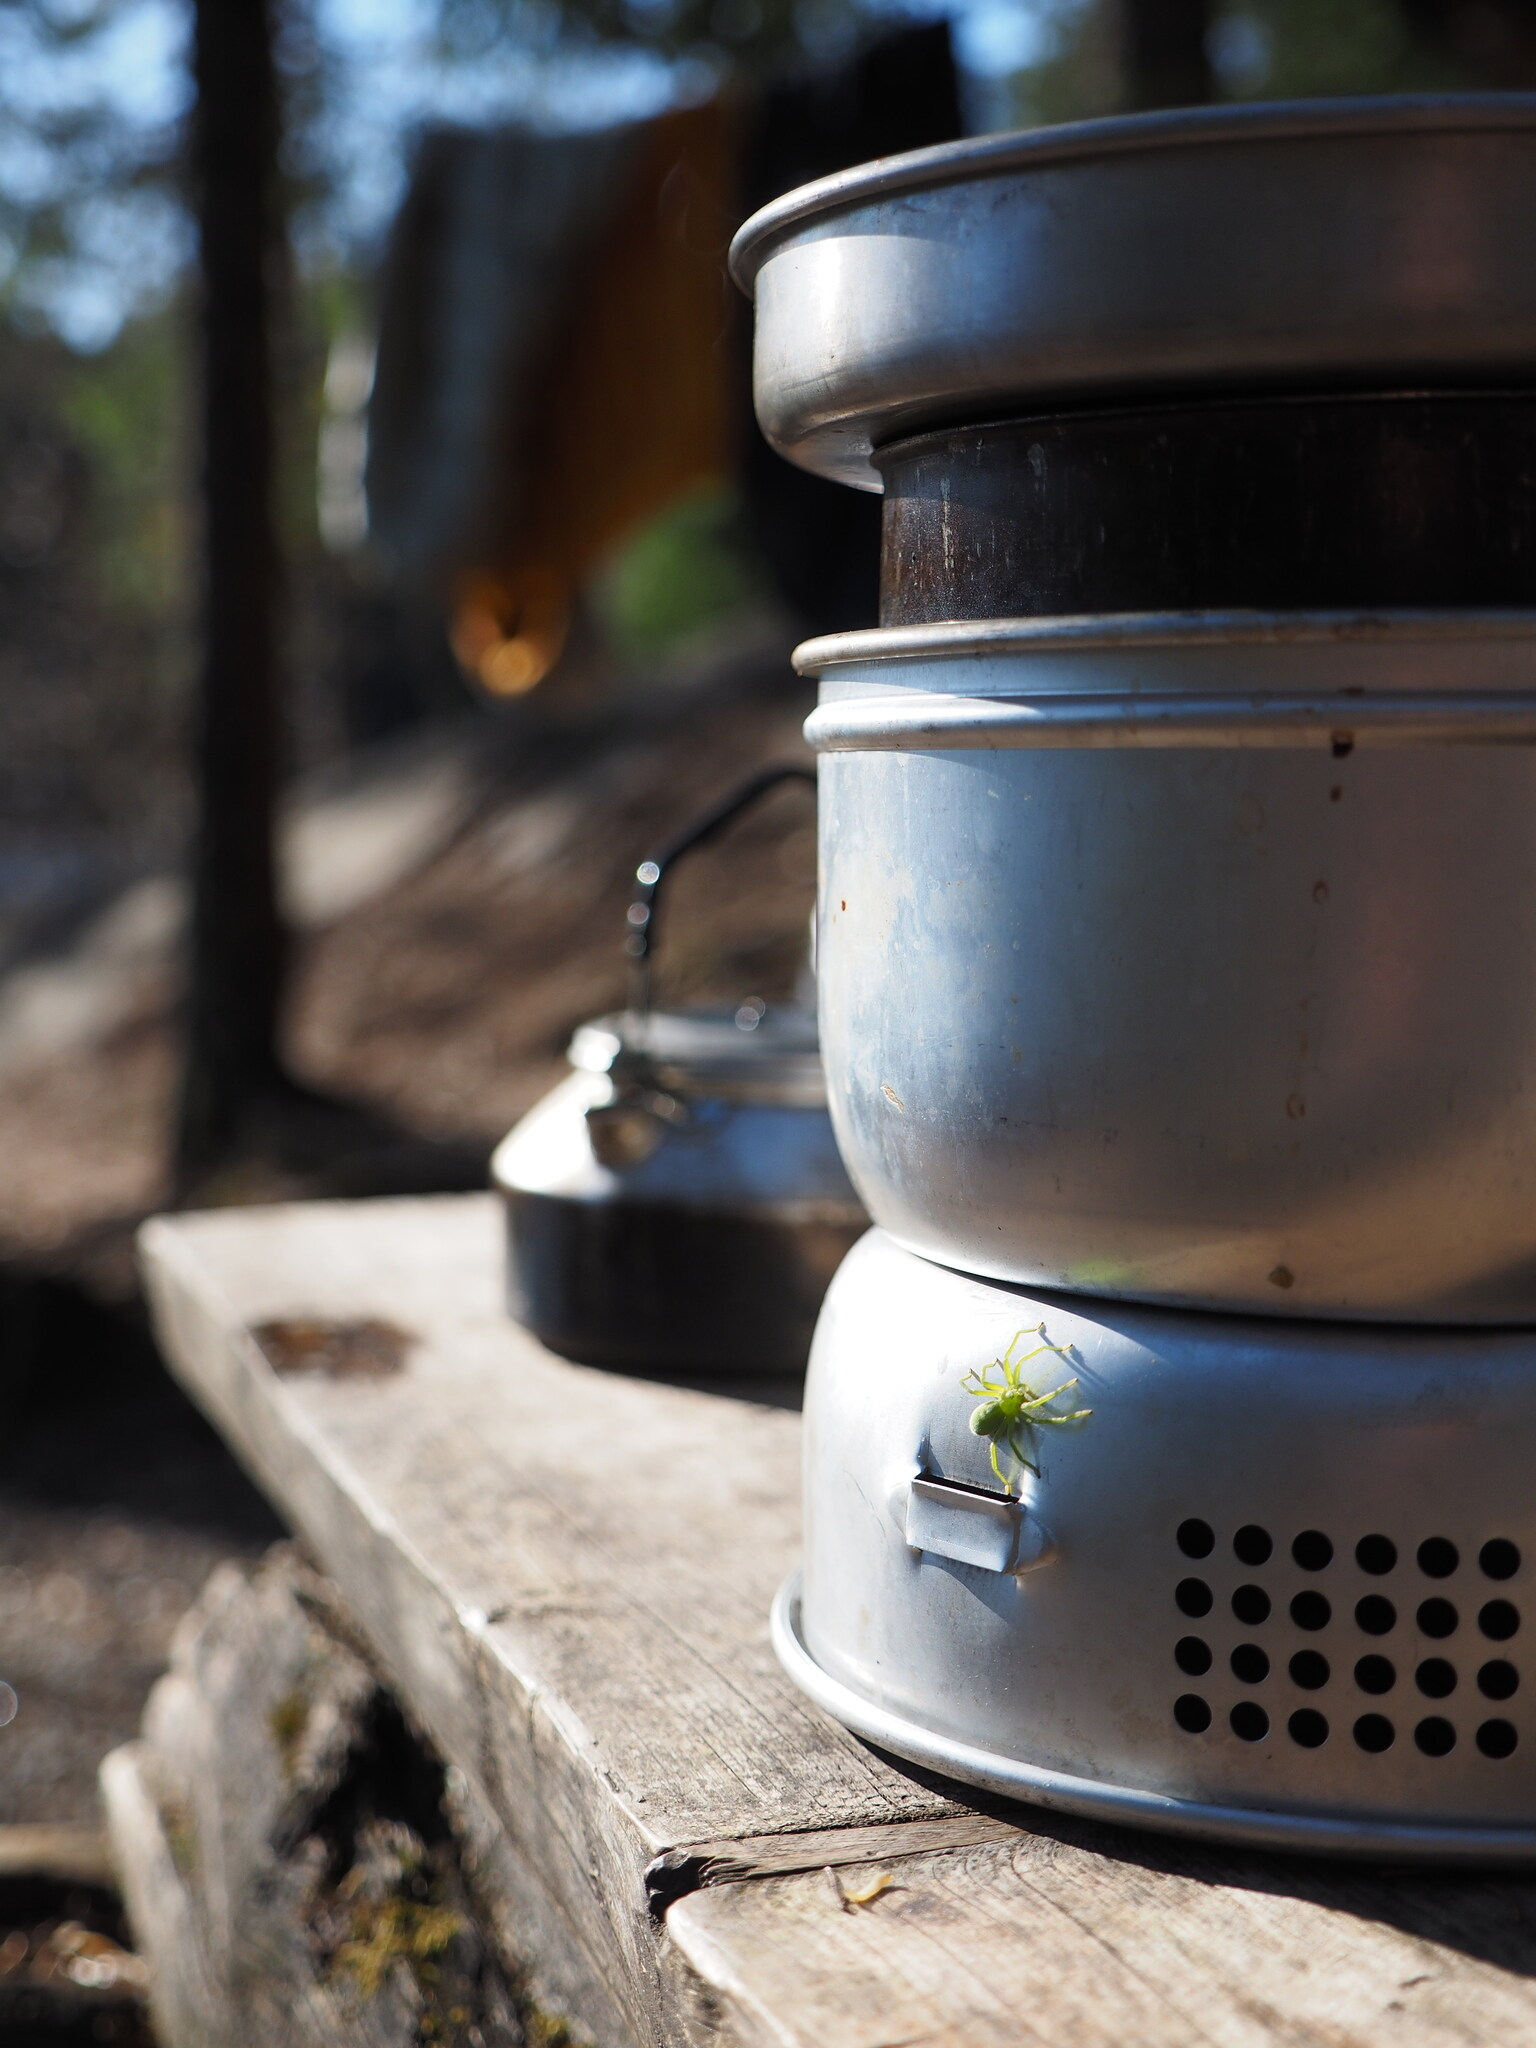
\includegraphics[height=0.36\paperheight]{assets/pyörävaellus17}
	\end{center}
	\columnbreak
	\begin{Figure}
		\noindent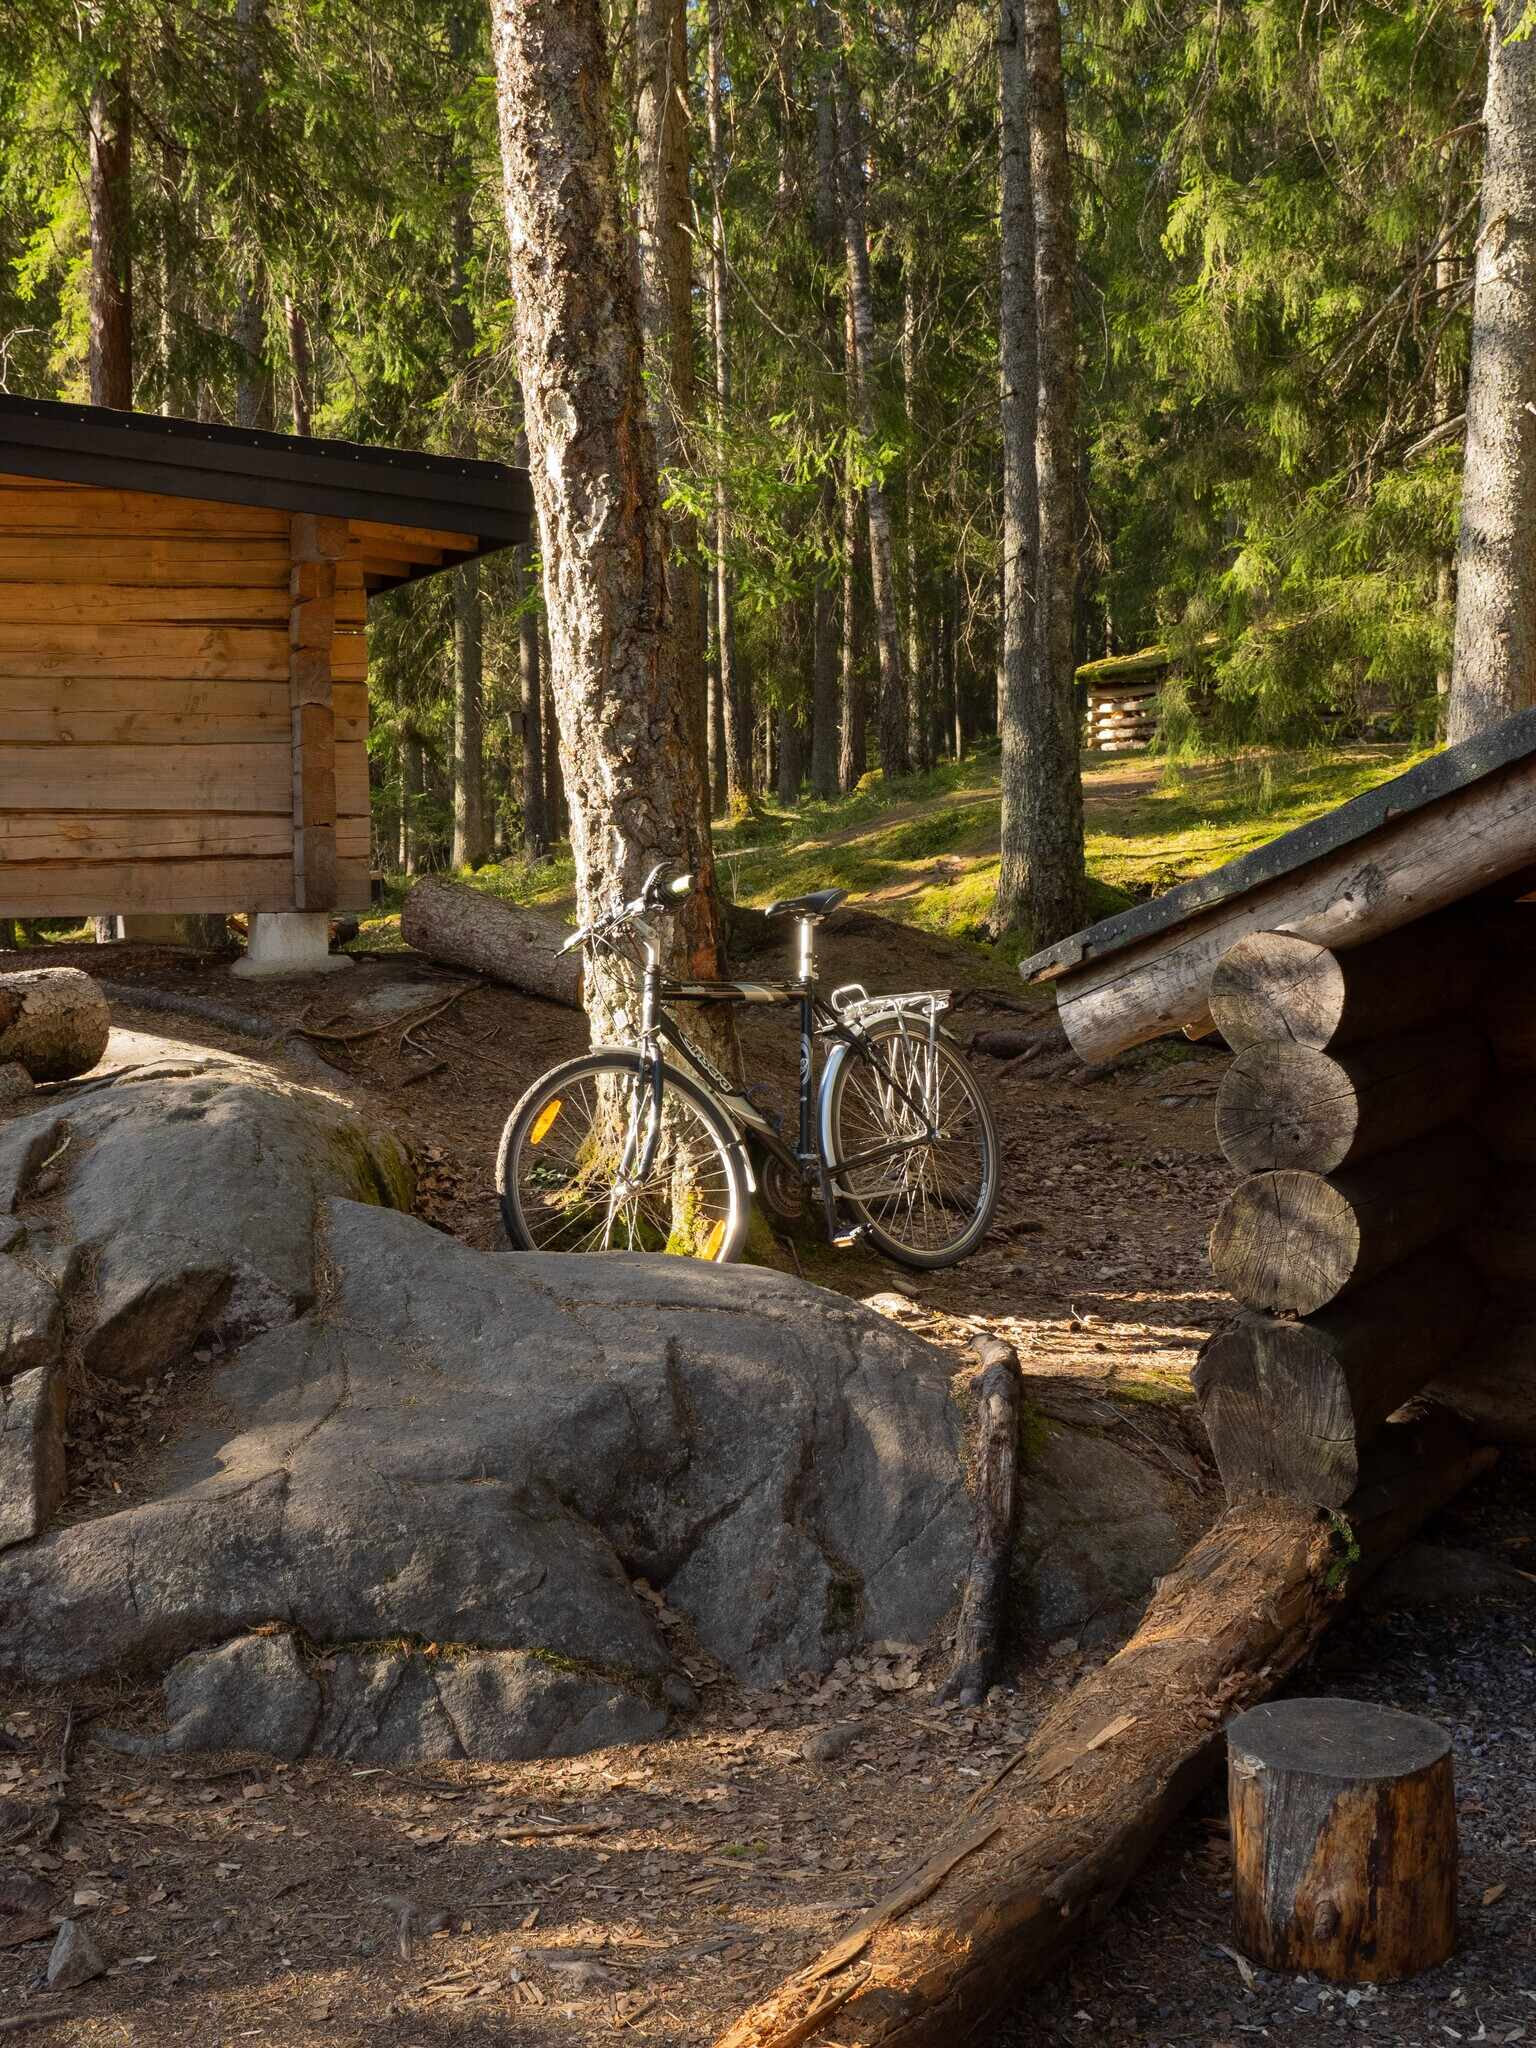
\includegraphics[height=0.36\paperheight]{assets/pyörävaellus18}
	\end{Figure}
\end{multicols}


\begin{Figure}
	\noindent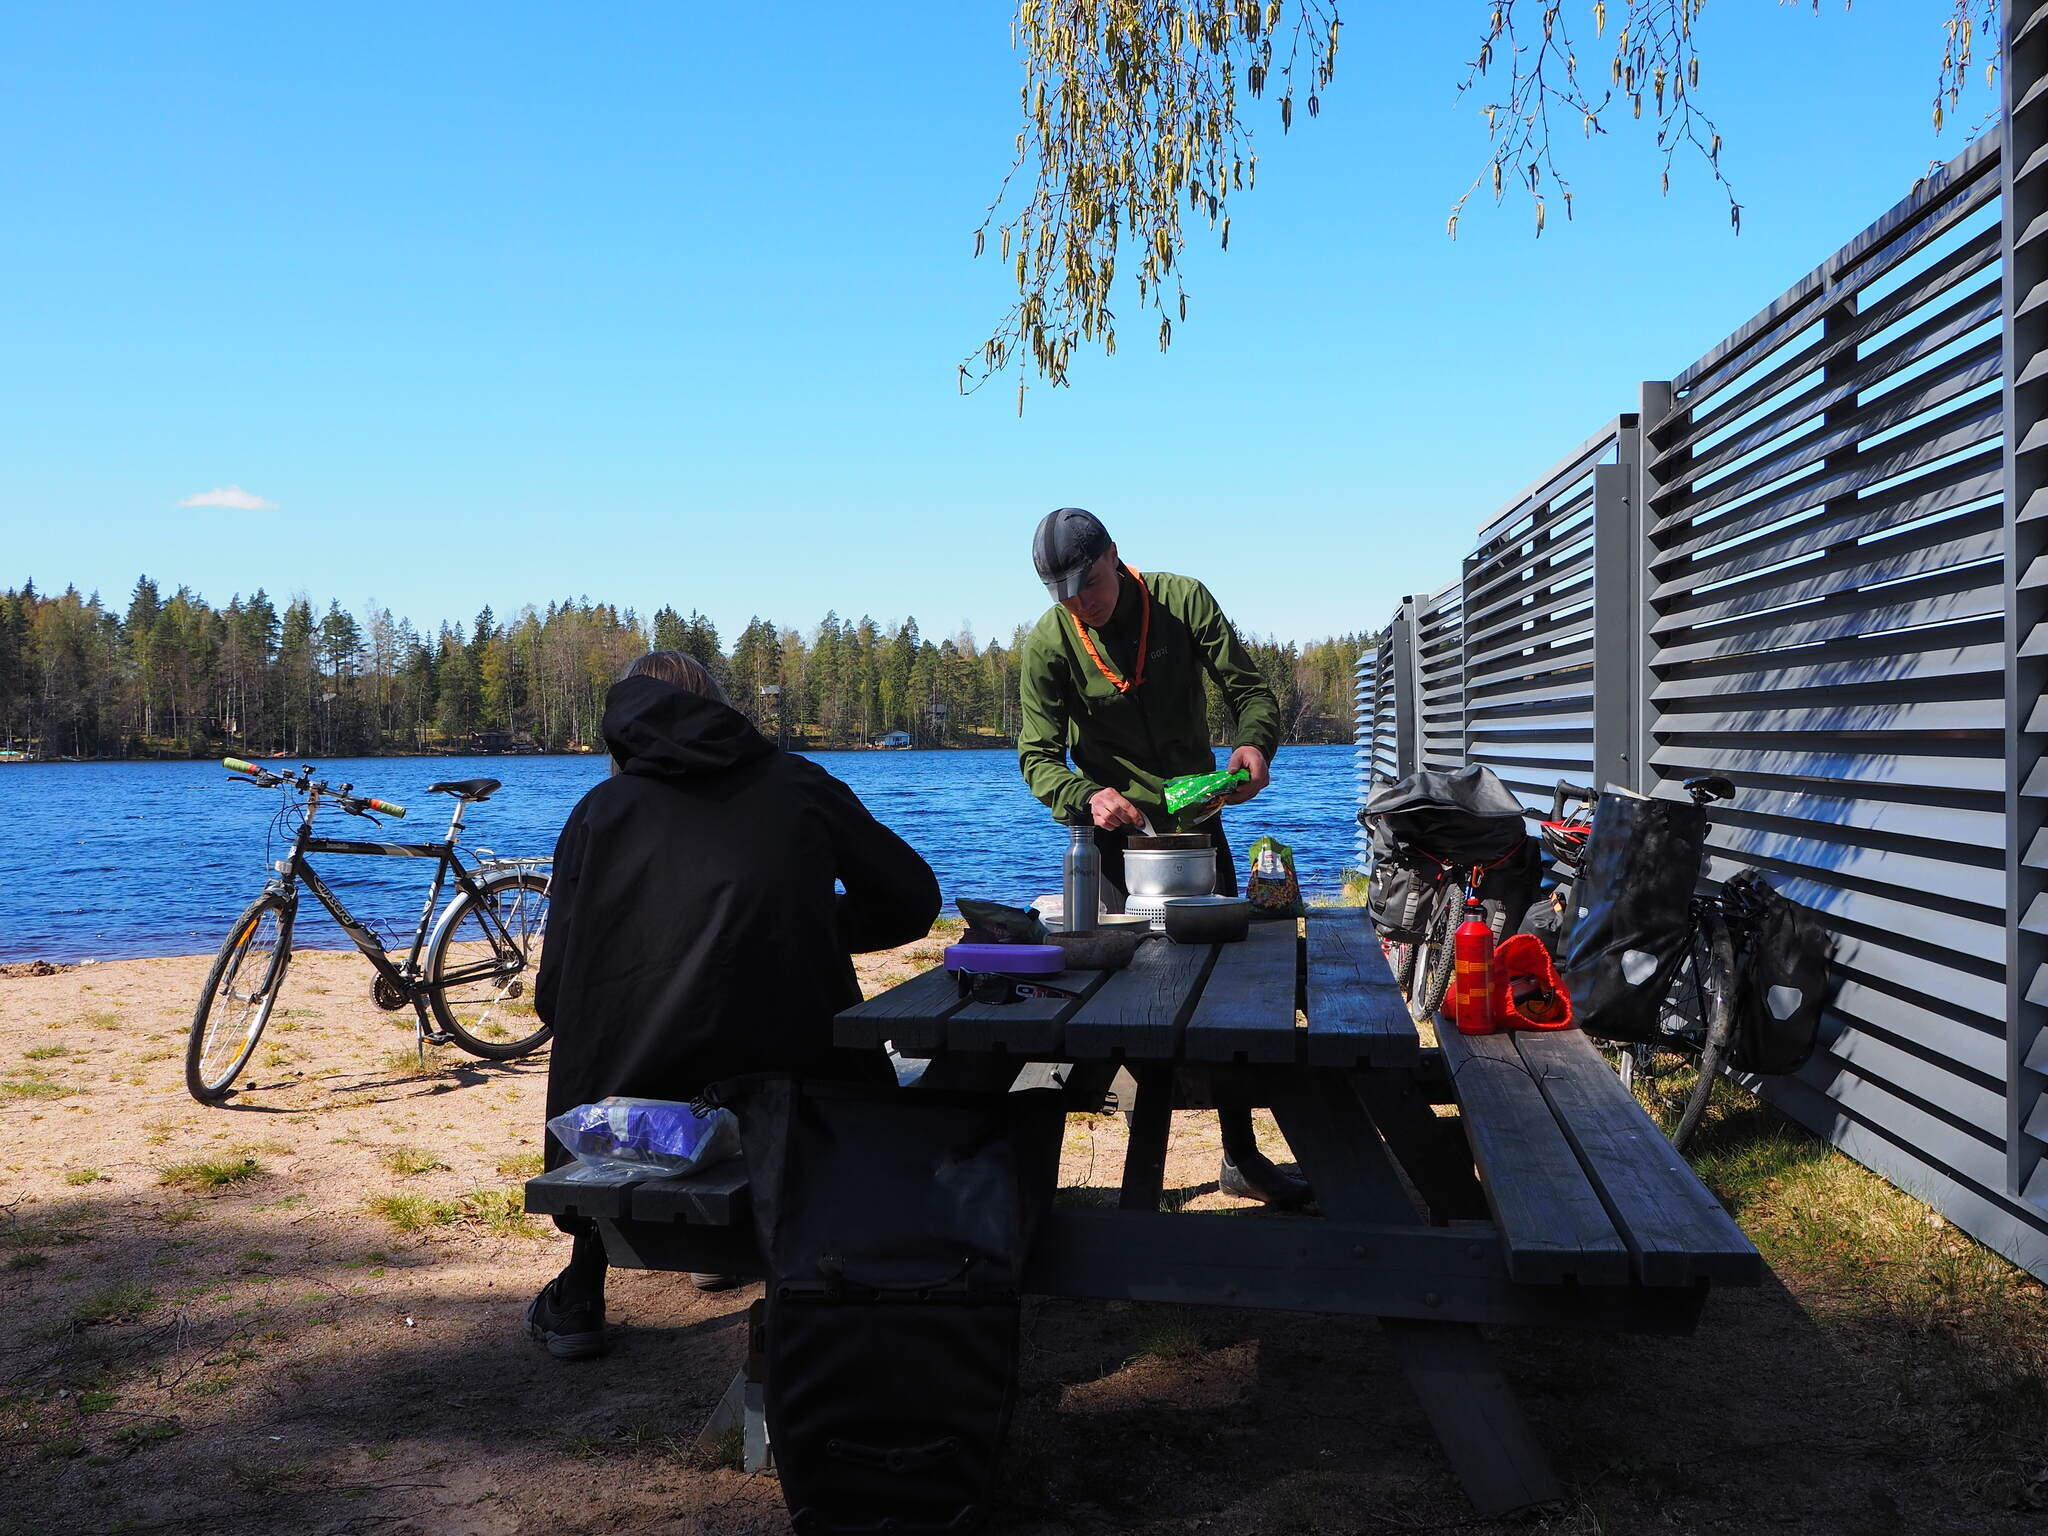
\includegraphics[width=\linewidth]{assets/pyörävaellus19}
	\captionof{figure}{Kolmas päivä oli taas aika pitkä, ja vei meidät itään, ensiksi Vihtiin. Lounastauko otettiin Nummelan Myllylammen uimarannalla, ja jatketiin matka kohti Espoon Vääräjärven.}
\end{Figure}

\begin{multicols}{2}
	\begin{center}
		\noindent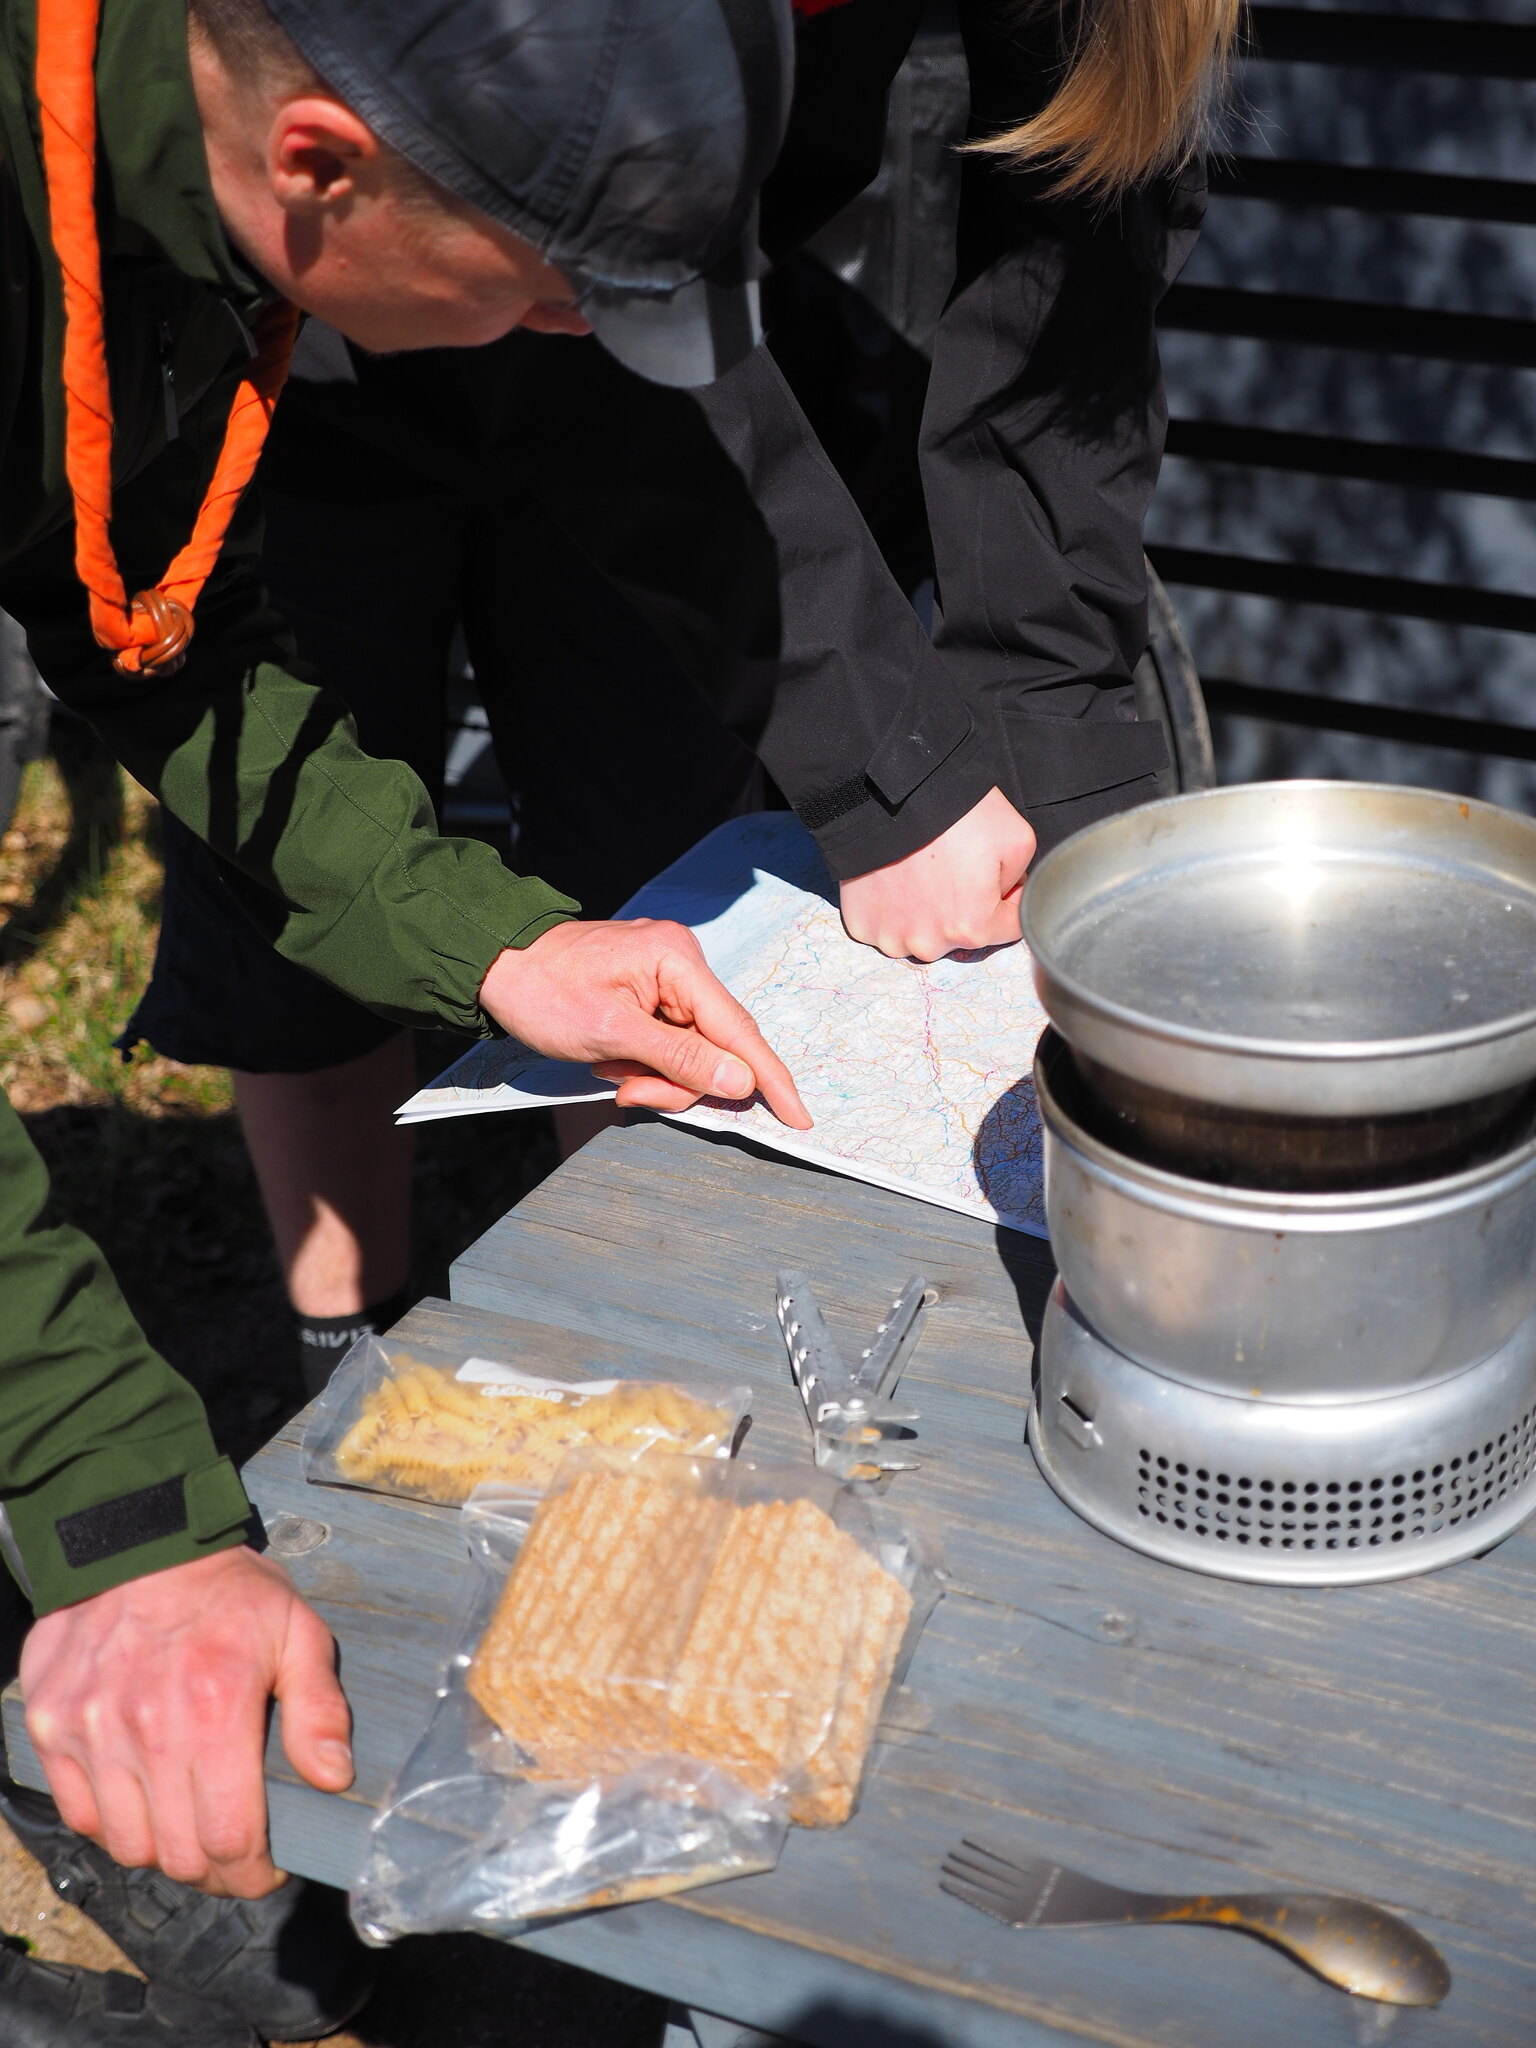
\includegraphics[height=0.36\paperheight]{assets/pyörävaellus20}
	\end{center}
	\columnbreak
	\begin{Figure}
		\noindent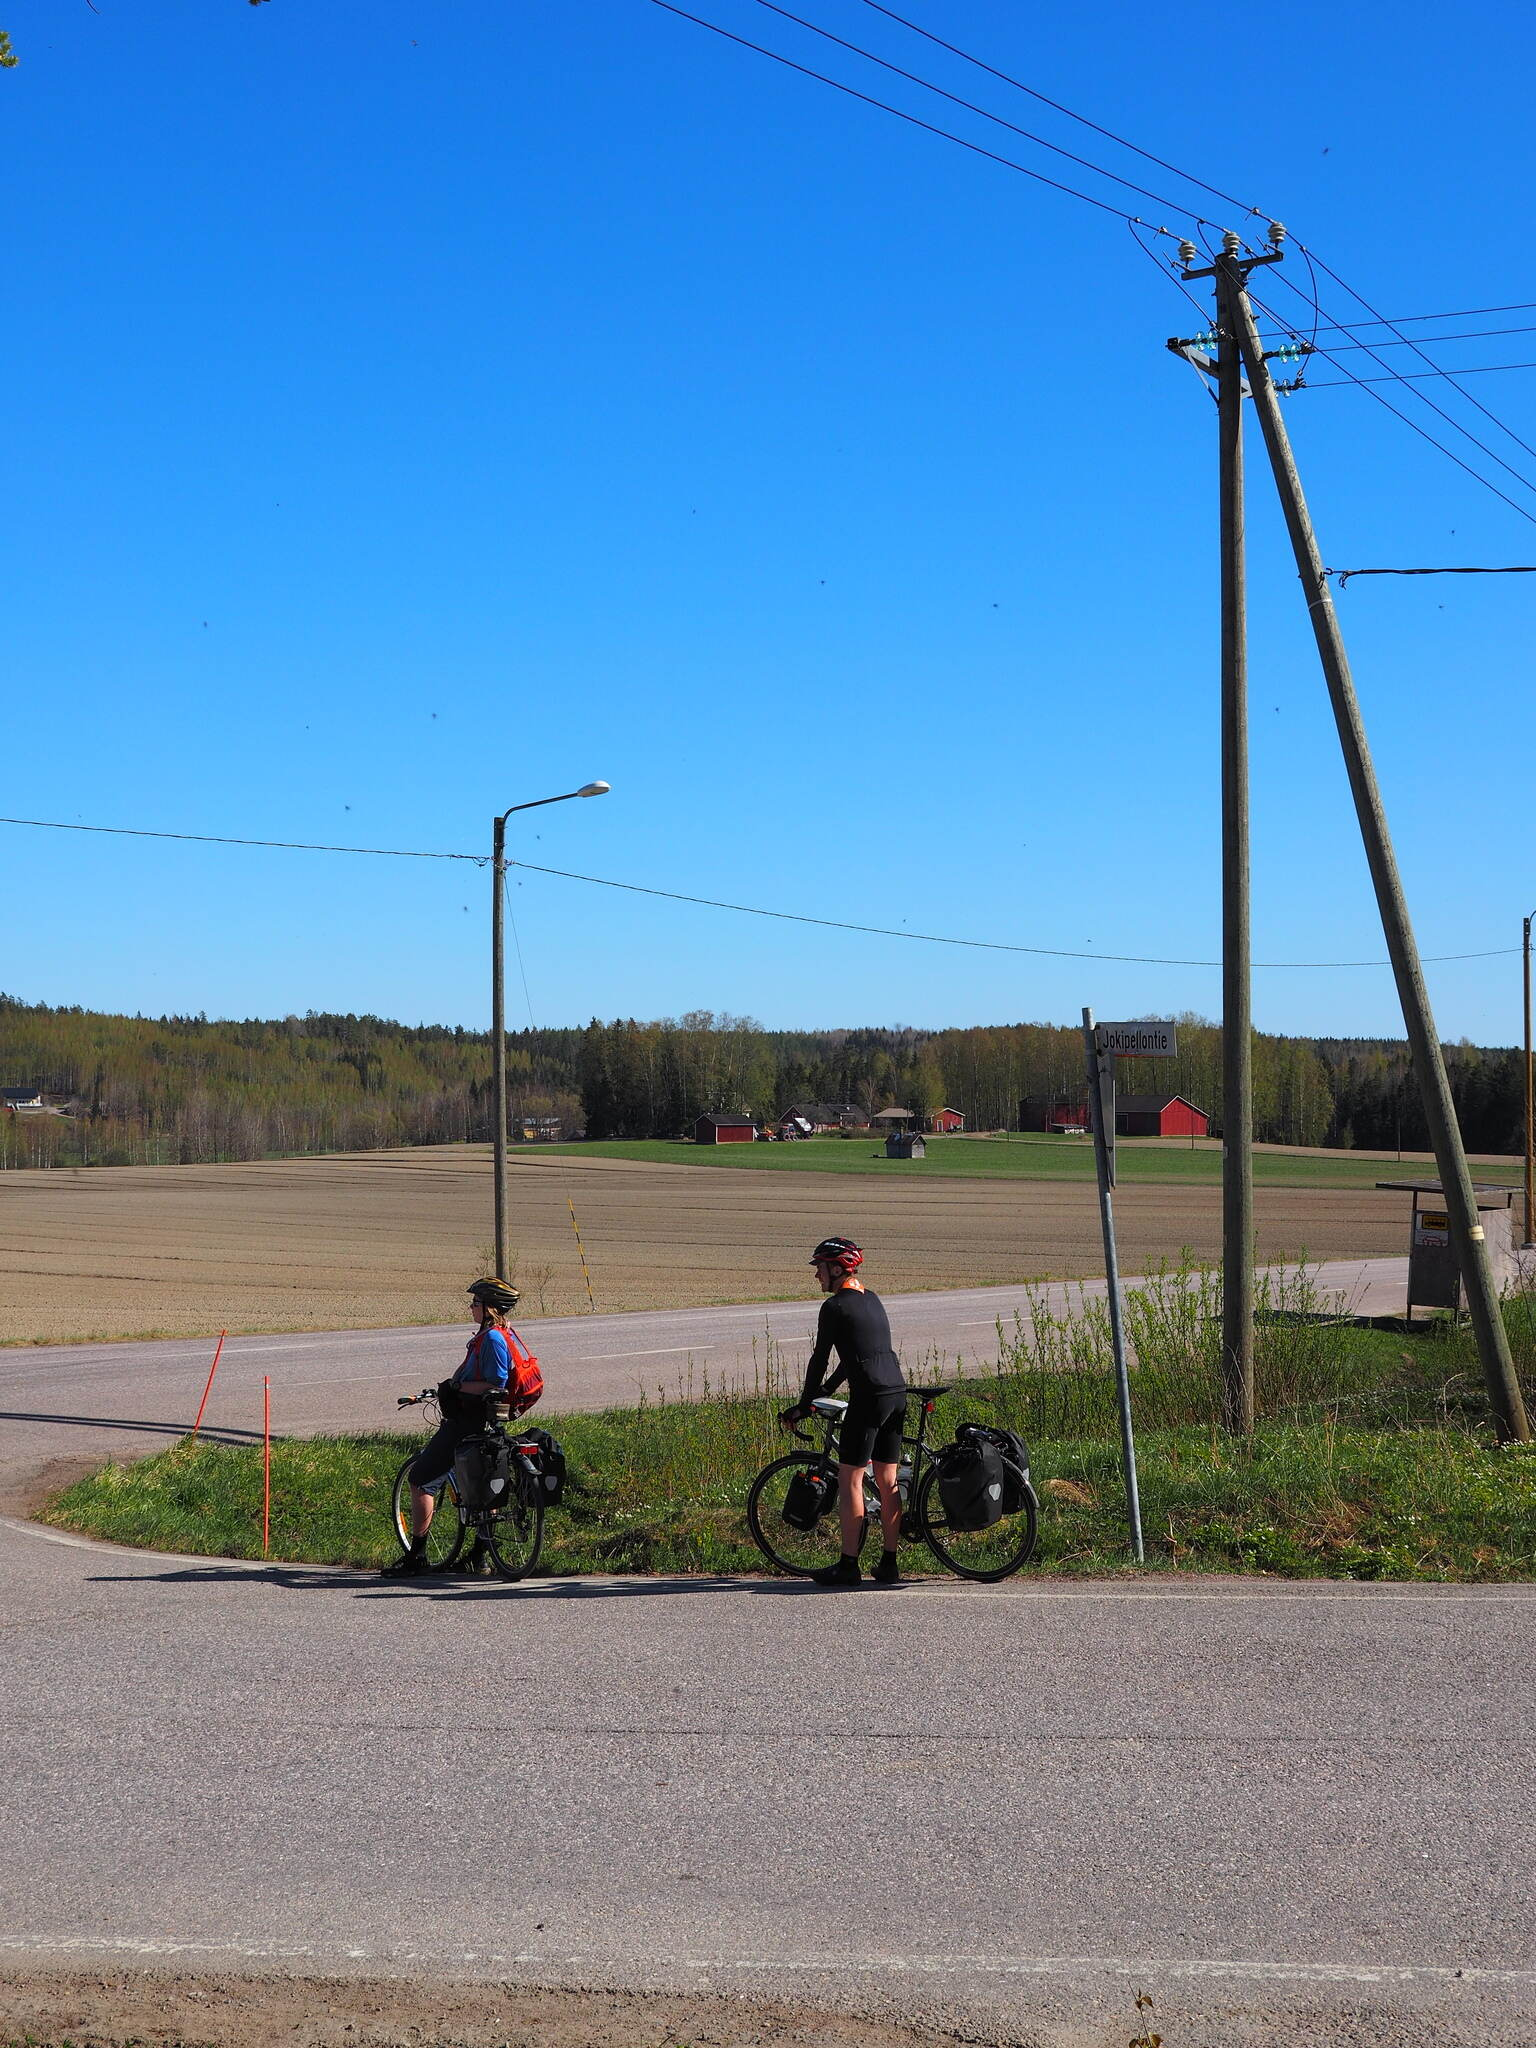
\includegraphics[height=0.36\paperheight]{assets/pyörävaellus21}
	\end{Figure}
\end{multicols}


\begin{multicols}{2}
	\begin{center}
		\noindent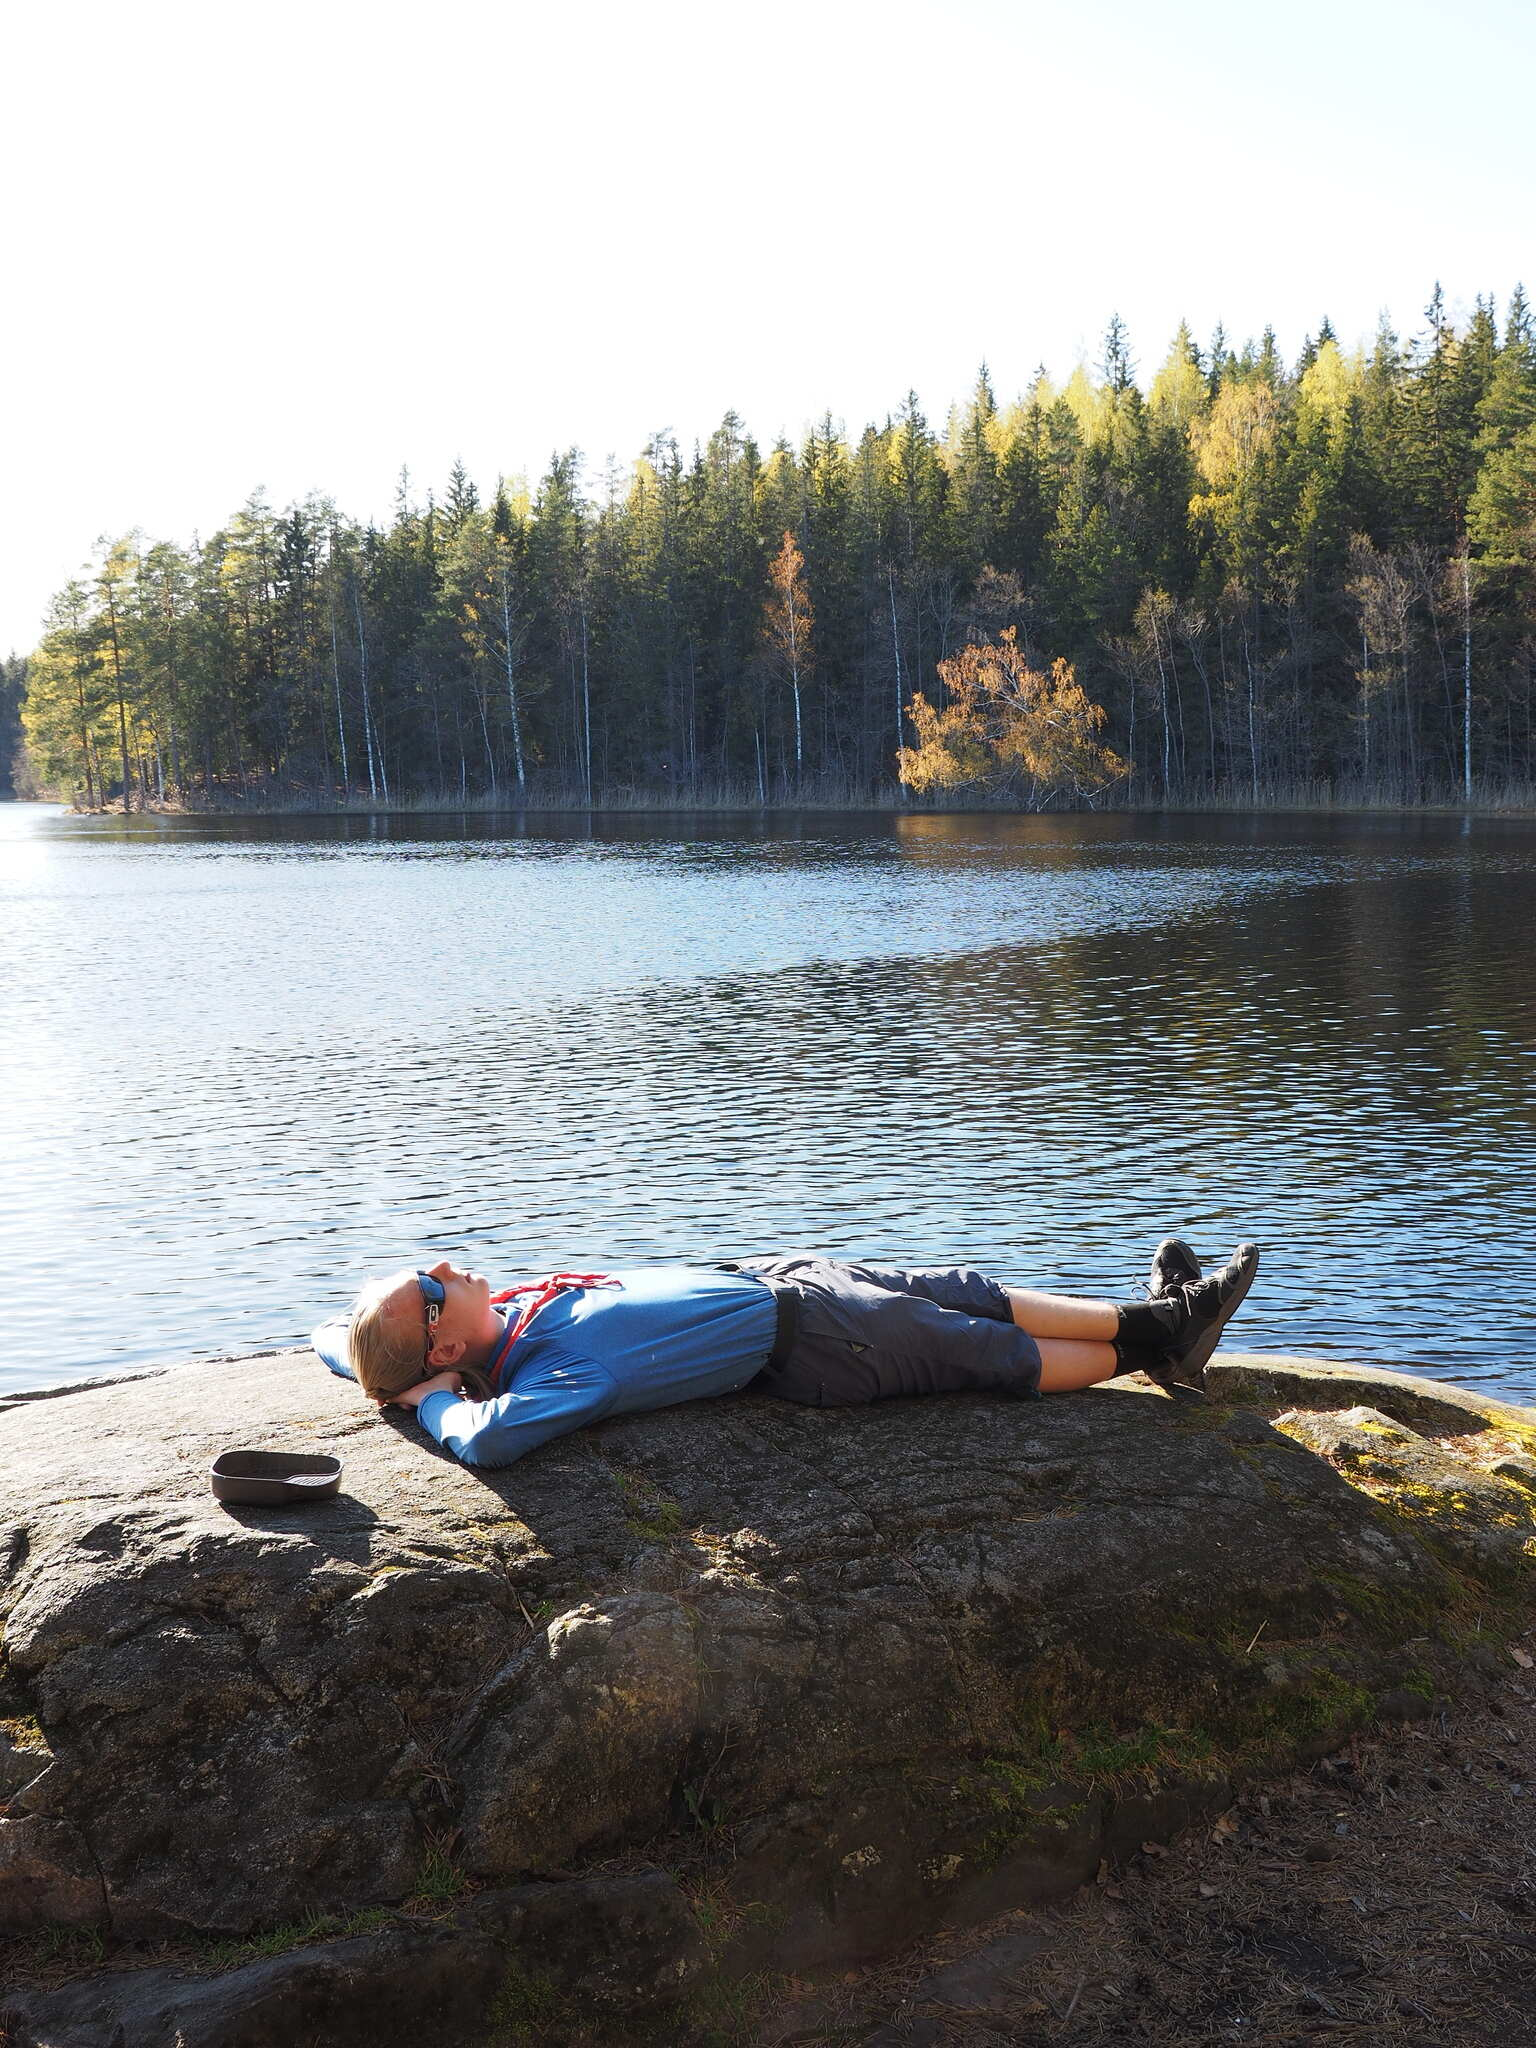
\includegraphics[width=1.05\linewidth]{assets/pyörävaellus24}
		\noindent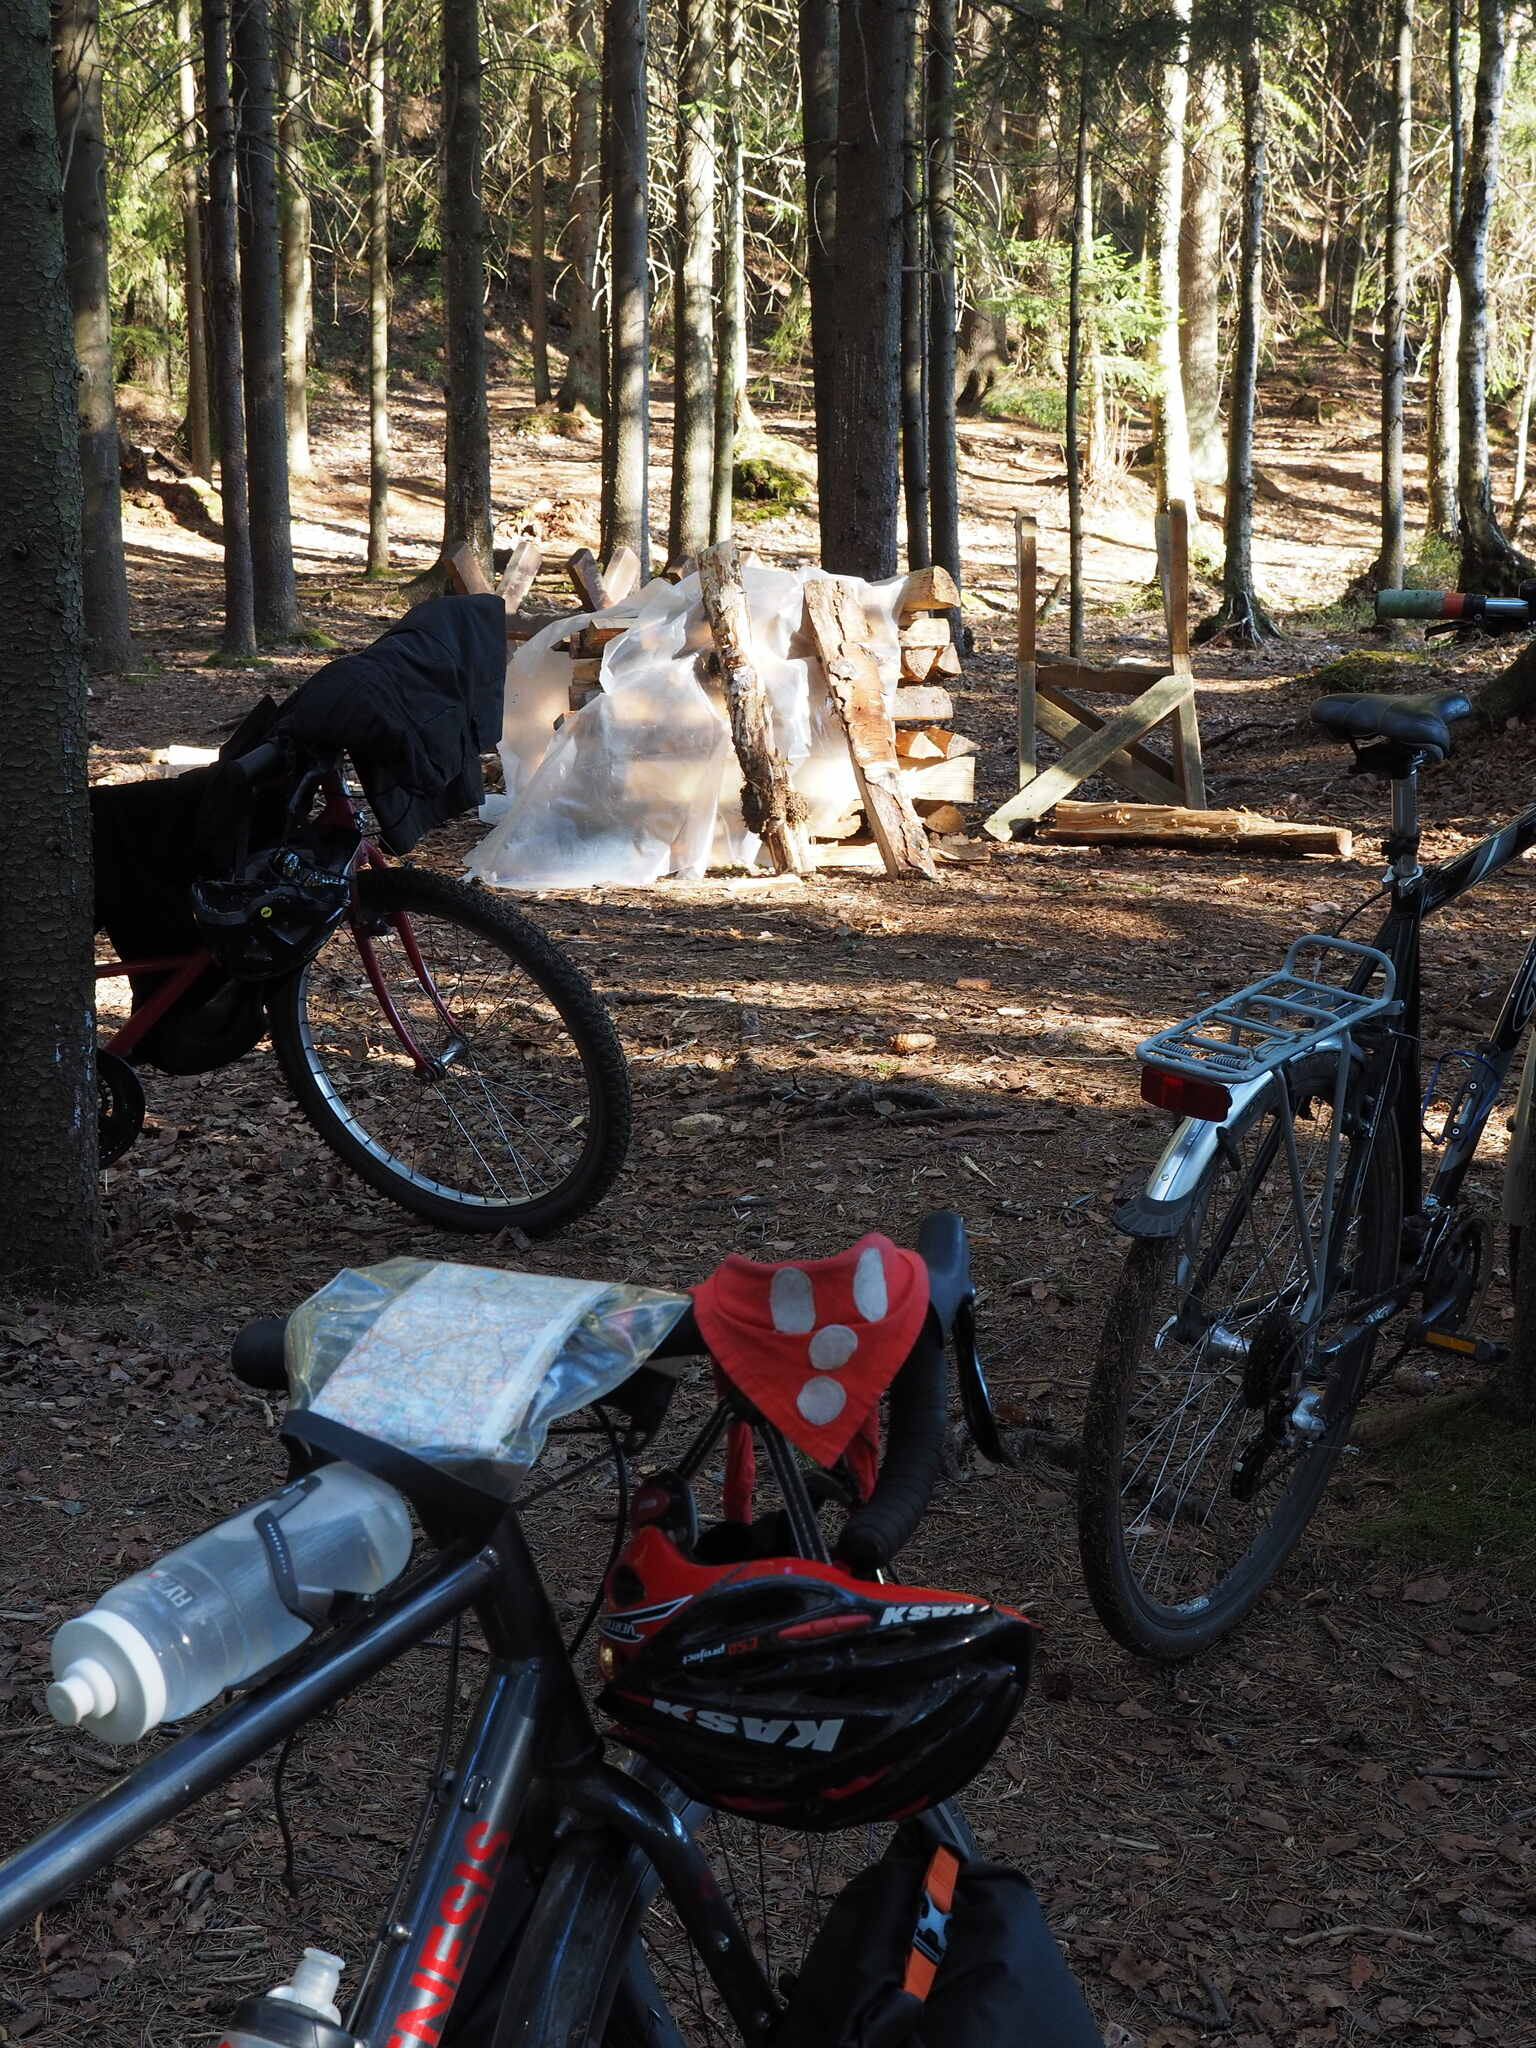
\includegraphics[width=1.05\linewidth]{assets/pyörävaellus22}
	\end{center}
	\columnbreak
	\begin{center}
		\noindent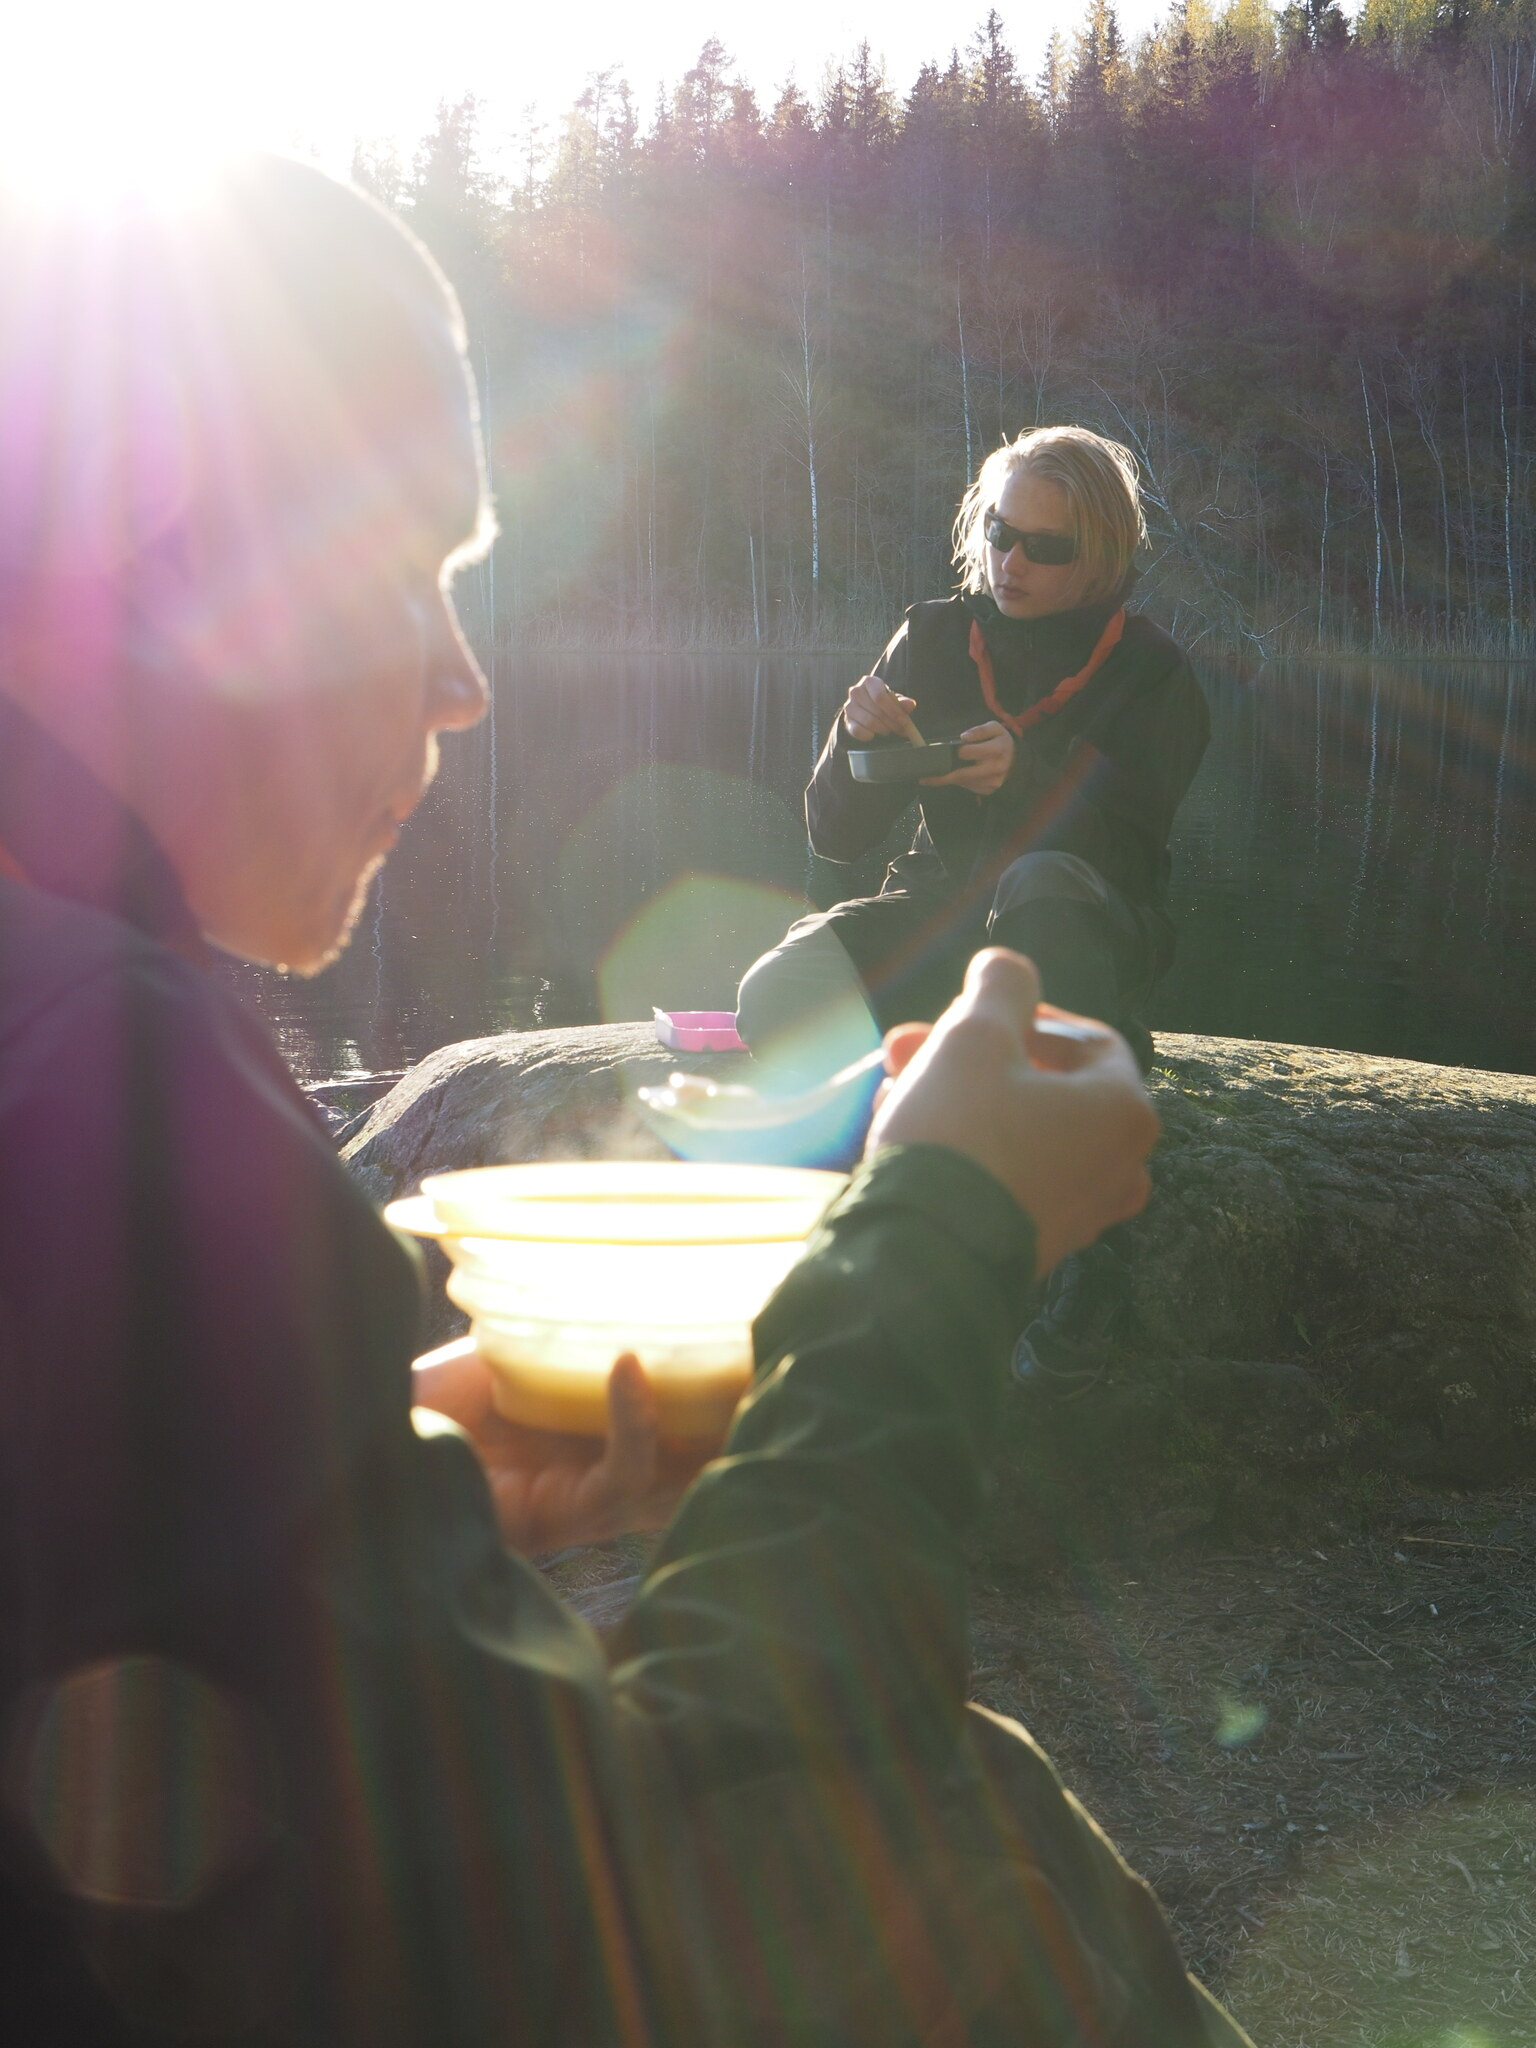
\includegraphics[width=1.05\linewidth]{assets/pyörävaellus23}
	\end{center}
	\begin{addmargin}[0.32cm]{0cm}
		{\small
		64km päivän jälkeen, saavuimme perille meidän viimeiseen
		yöpymispaikkaan: Vääräjärvi, Espoo}
	\end{addmargin}
\end{multicols}


\begin{multicols}{2}
	\begin{center}
		\noindent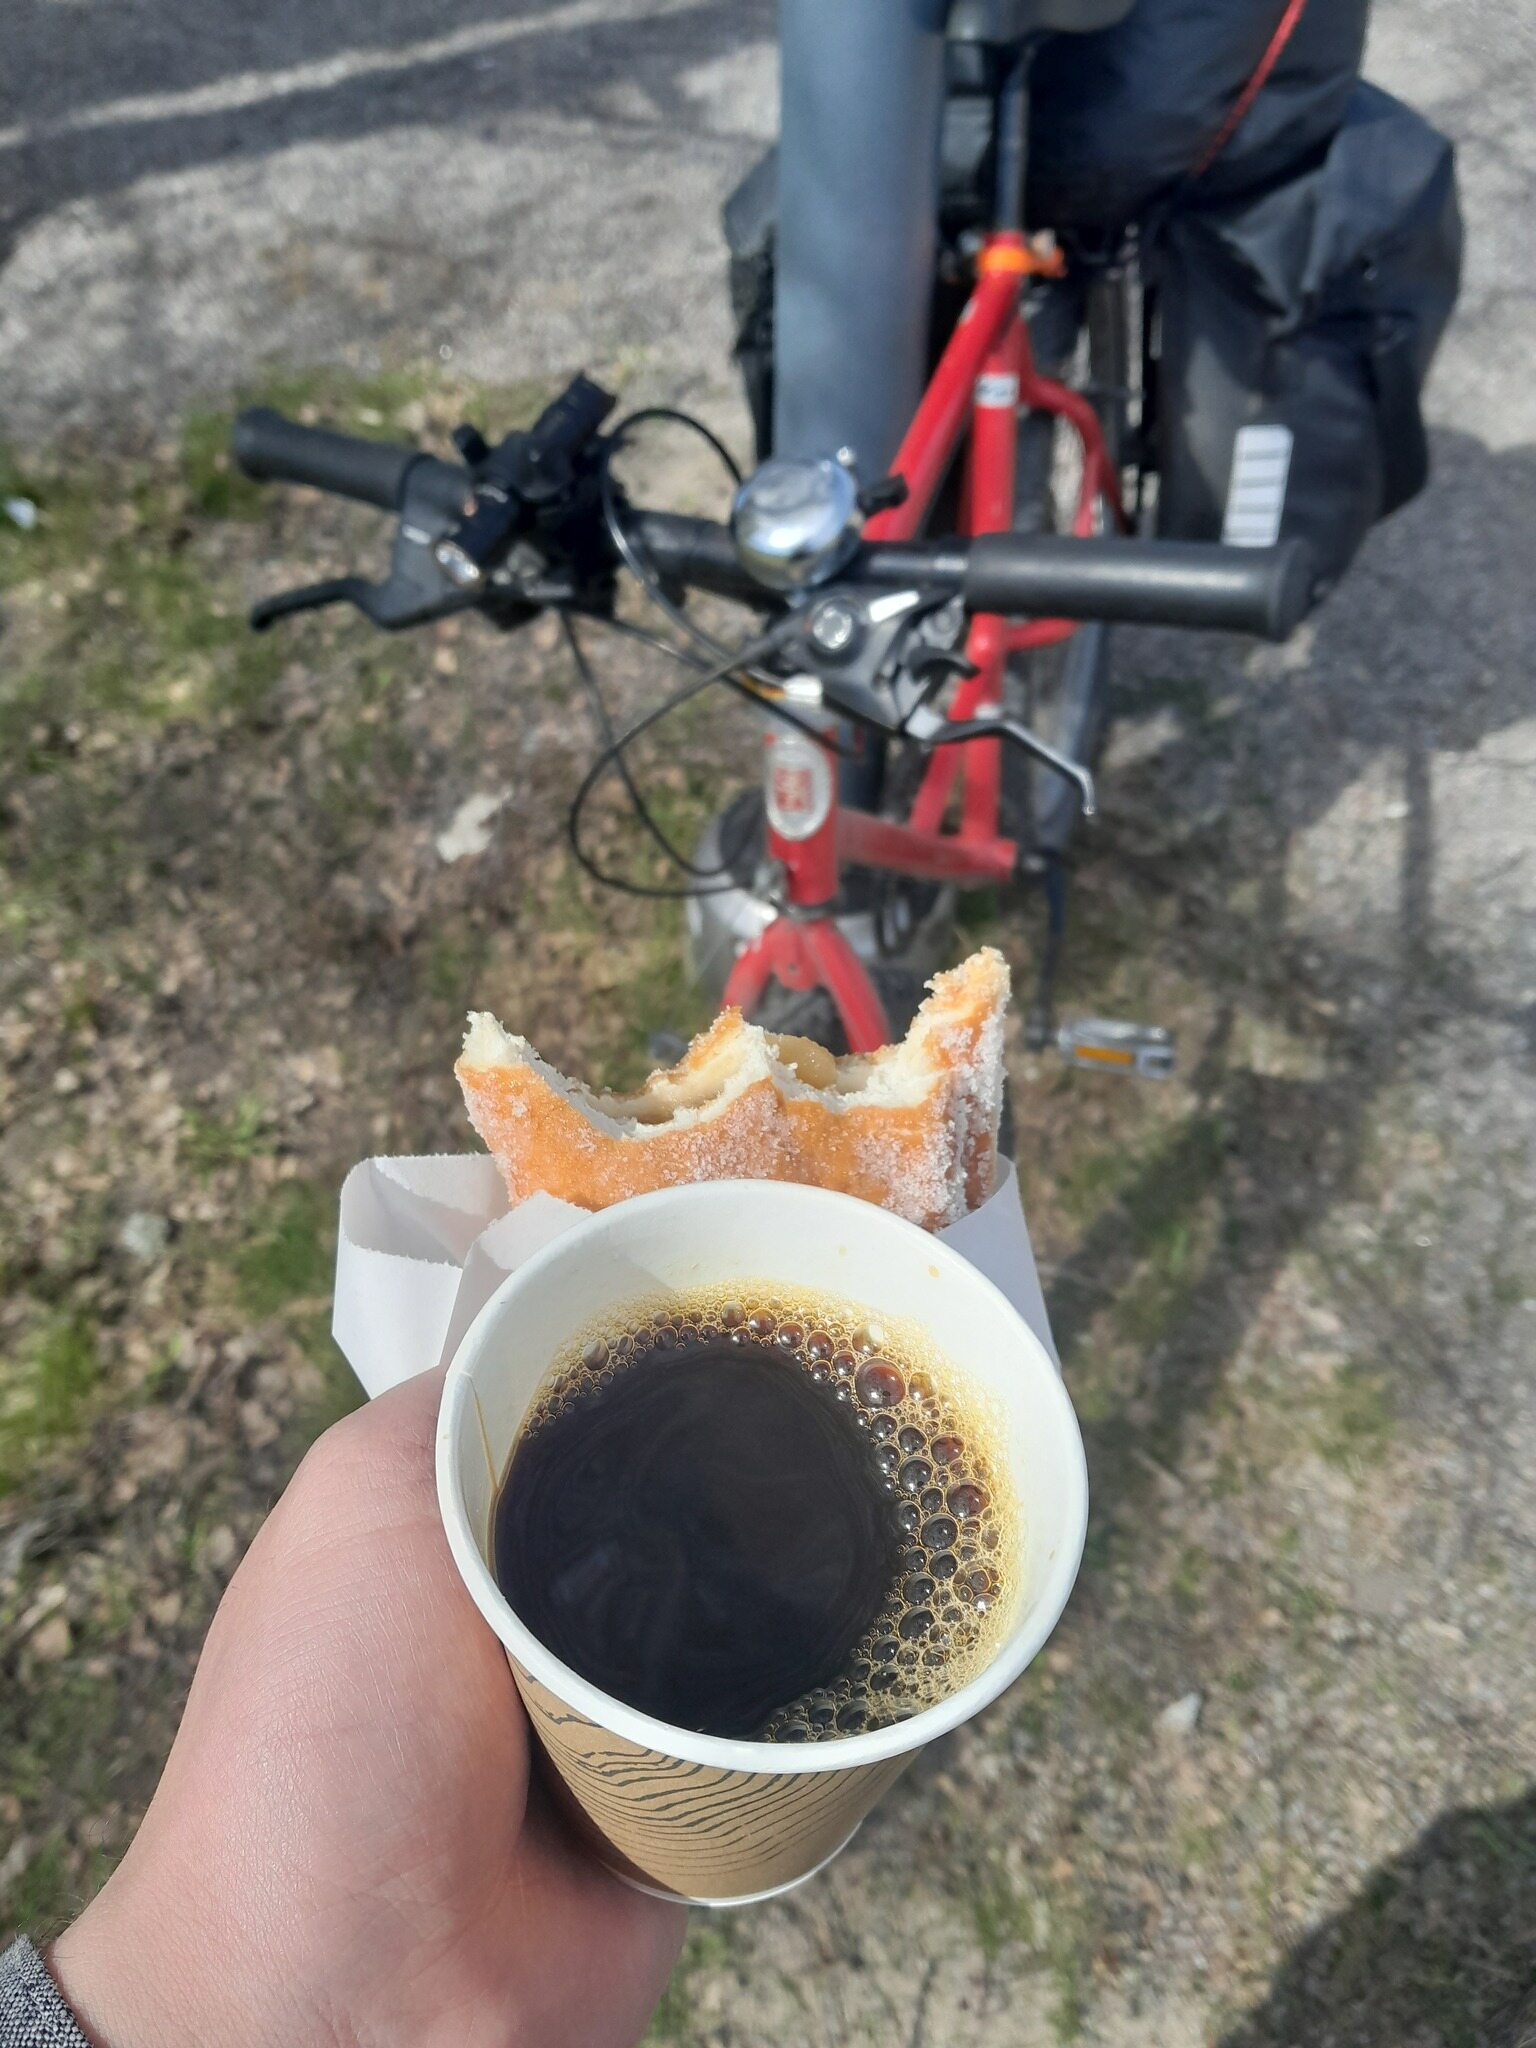
\includegraphics[width=1.05\linewidth]{assets/pyörävaellus25}
		\noindent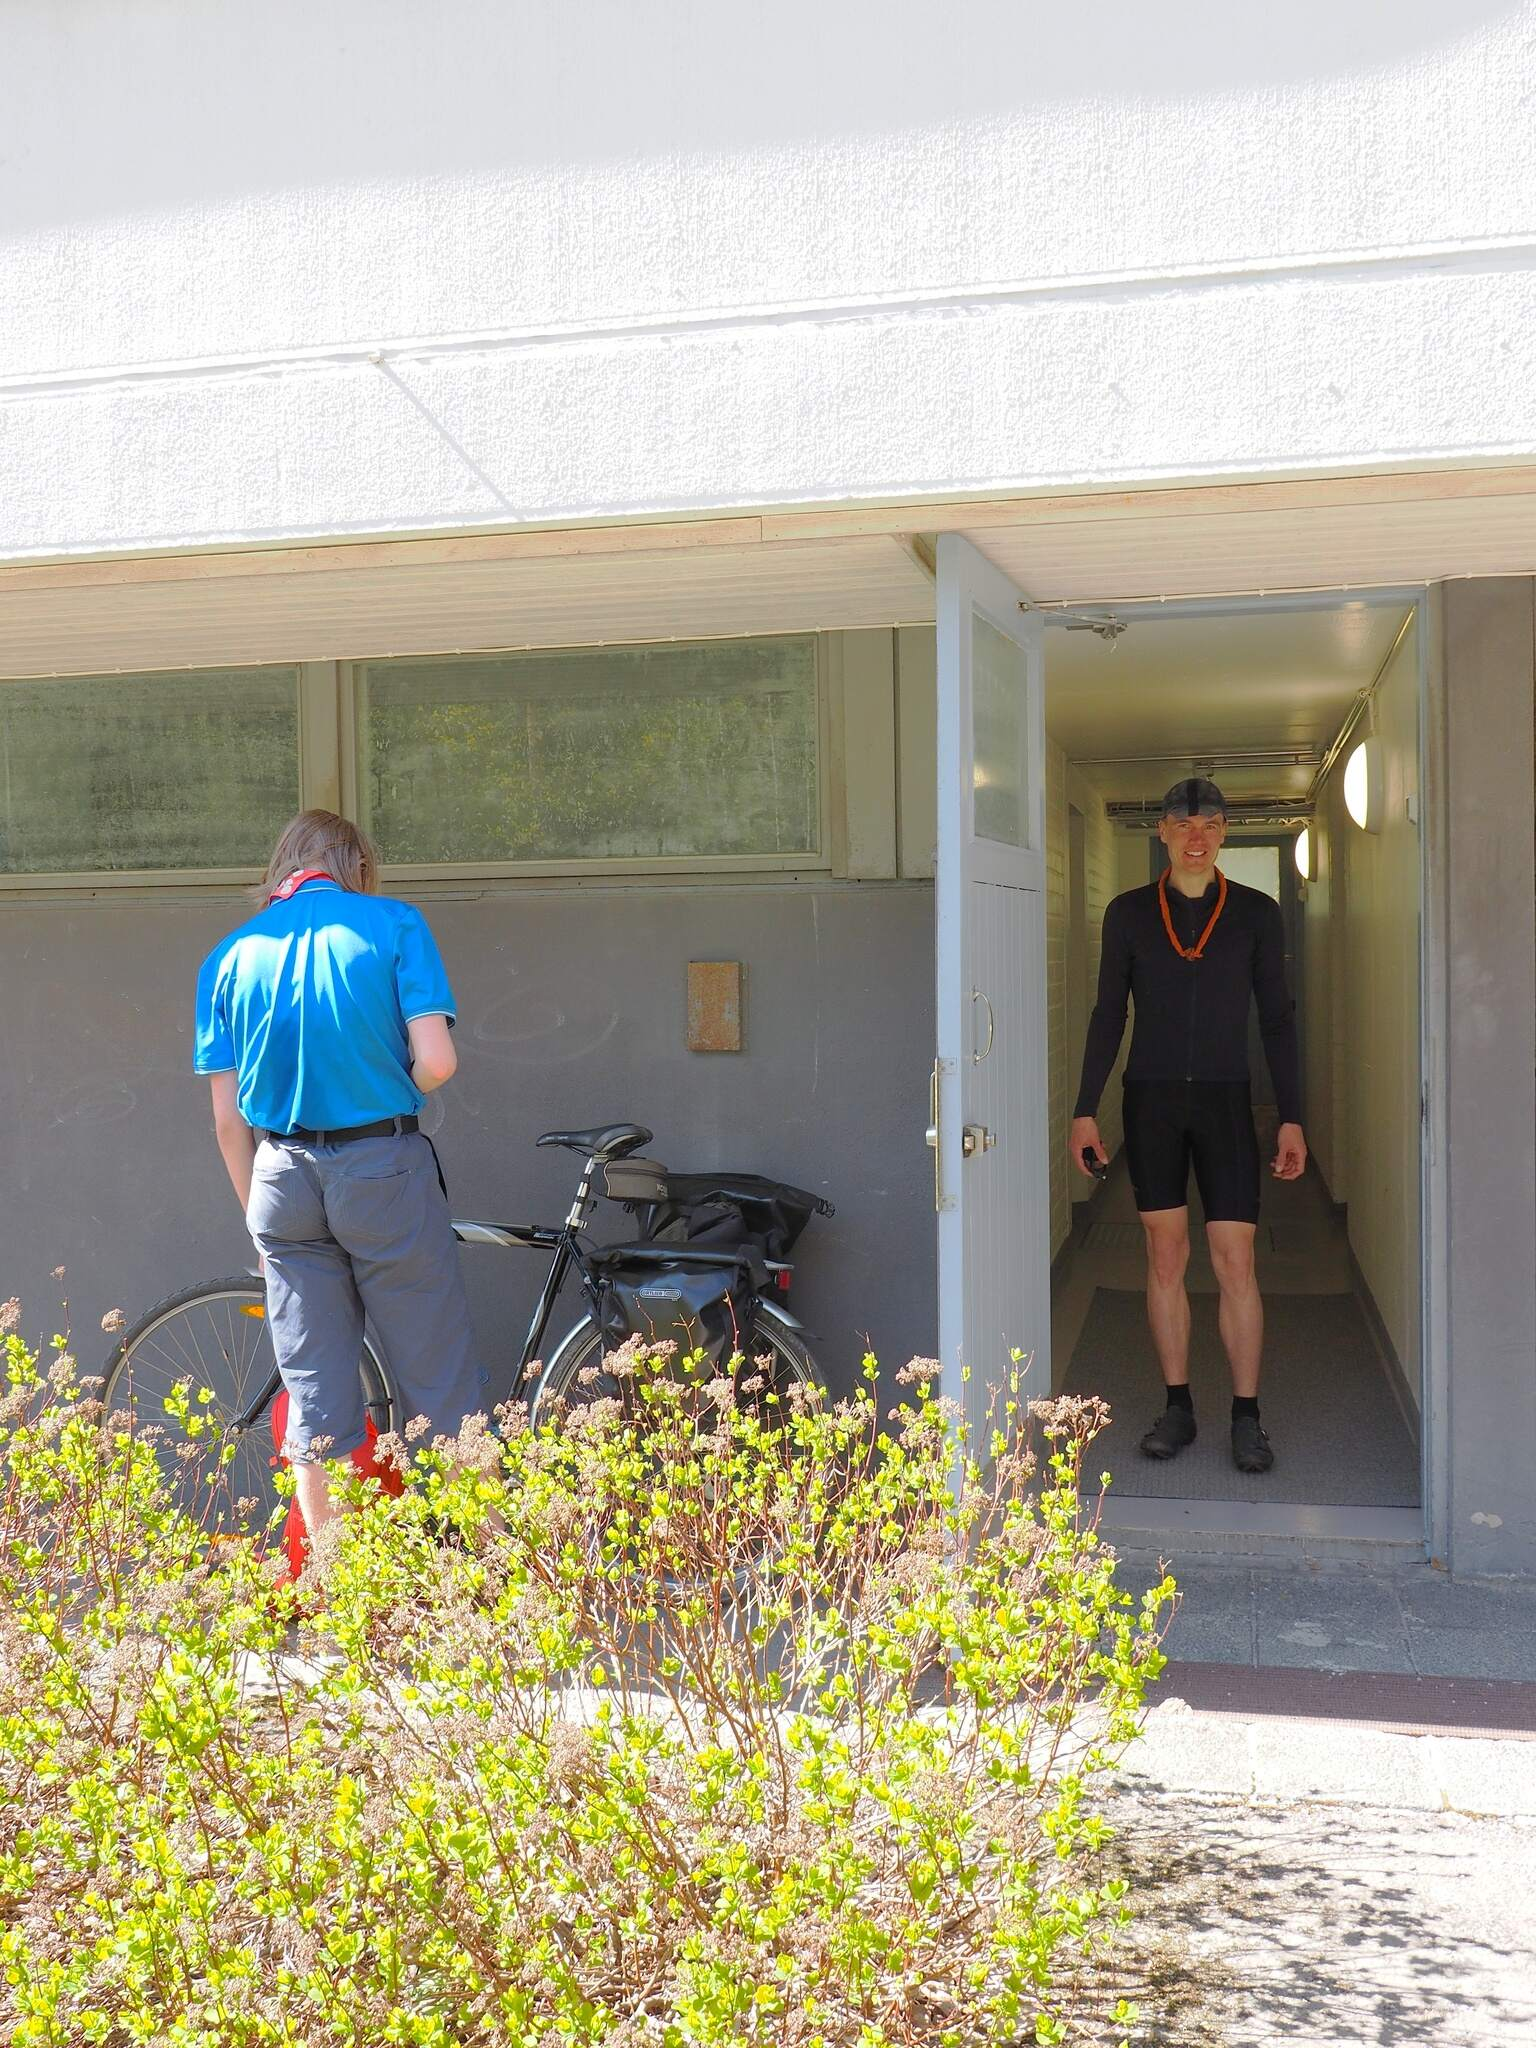
\includegraphics[width=1.05\linewidth]{assets/pyörävaellus26}
	\end{center}
	\columnbreak
	\vspace*{0.32cm}
	\begin{center}
		\noindent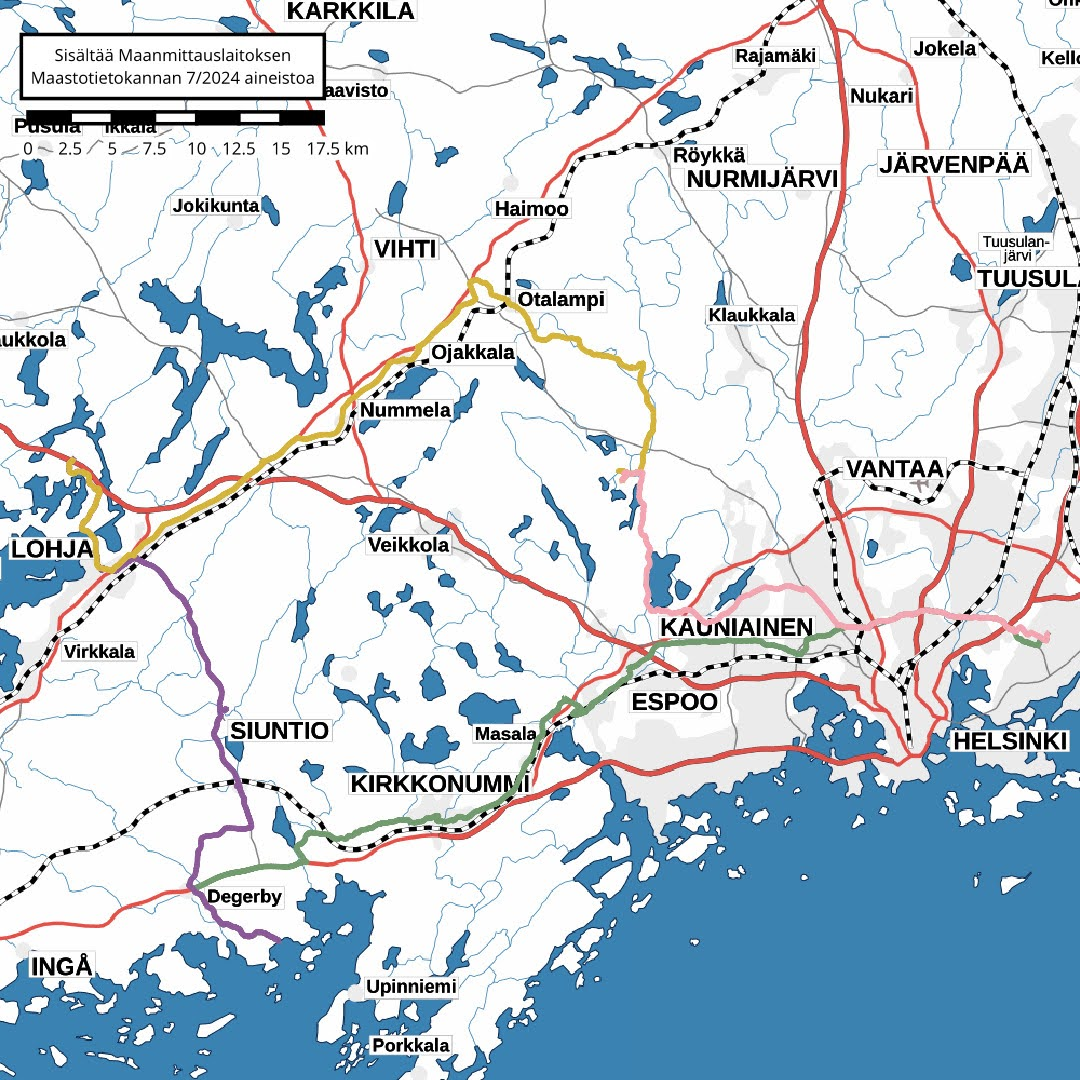
\includegraphics[width=1.05\linewidth]{assets/pyörävaellus27}
	\end{center}
	\vspace*{2cm}
	\begin{addmargin}[0.32cm]{0cm}
		{\small
		Neljäs ja viimeinen päivä meni nopeasti, ja meillä oli ''väin'' 39km
		jäljellä Kontulaan.
		Skipattiin lounas, ja otettiin sen sijaan muutaman
		välipalatauon. Nopeammin kuin osaisimme uskoa, olimme takaisin
		varastossa, 224km takanamme!
		}
	\end{addmargin}
\end{multicols}
\vspace*{-0.32cm}


\medskip
\noindent\null\hfill Tanguy Gérôme
